\documentclass[12pt, a4paper]{article}
\usepackage{amsfonts, amsmath, amssymb, amsthm}
\usepackage{enumitem}
\usepackage{mathtools}
\usepackage{fullpage}
\usepackage{mathrsfs}
\theoremstyle{plain}
\newtheorem{innercustomgeneric}{\customgenericname}
\providecommand{\customgenericname}{}
\newcommand{\newcustomtheorem}[2]{%
\newenvironment{#1}[1]{
\renewcommand\customgenericname{#2}%
\renewcommand\theinnercustomgeneric{##1}%
\innercustomgeneric
}
{\endinnercustomgeneric}
}
\newcustomtheorem{lemma}{Lemma}

\makeatletter
\newcommand*\bigcdot{\mathpalette\bigcdot@{.5}}
\newcommand*\bigcdot@[2]{\mathbin{\vcenter{\hbox{\scalebox{#2}{$\m@th#1\bullet$}}}}}
\makeatother

\setcounter{section}{1}

\newcommand{\vertiii}[1]{{\left\vert\kern-0.25ex\left\vert\kern-0.25ex\left\vert #1 
    \right\vert\kern-0.25ex\right\vert\kern-0.25ex\right\vert}}
\makeatletter

\newcommand{\N}{\mathbb{N}}
\newcommand{\Hs}{\mathbb{H}}
\newcommand{\A}{\mathscr{A}}
\newcommand{\B}{\mathscr{B}}
\newcommand{\U}{\mathscr{U}}
\newcommand{\Q}{\mathbb{Q}}
\newcommand{\R}{\mathbb{R}}
\newcommand{\Z}{\mathbb{Z}}
\newcommand{\C}{\mathbb{C}}
\newcommand{\set}[1]{\mathbb{#1}}
\newcommand{\F}{\mathcal{F}}
\newcommand{\T}{\mathcal{T}}
\newcommand{\G}{\mathcal{G}}
\newcommand{\card}{\mathbf{card}}
\DeclareMathOperator{\inter}{Int} 

\usepackage{xcolor}
\usepackage{mdframed}
\usepackage{indentfirst}
\usepackage{hyperref}
\newenvironment{exercise}[2][Exercise]
    { \begin{mdframed}[backgroundcolor=gray!20] \textbf{#1 #2} \\}
    {  \end{mdframed}}
    
\newenvironment{problem}[2][Problem]
    { \begin{mdframed}[backgroundcolor=gray!20] \textbf{#1 #2} \\}
    {  \end{mdframed}}

\title{Answer to Real Analysis by Carothers}
\author{Hoang Vo Ke}
\date{\today}

\begin{document}

\maketitle

\section*{Chapter 4. Open Sets and Closed Sets}

\begin{exercise}{3}
Some authors say that two metrics $d$ and $p$ on a set $M$ are equivalent if they generate the same open sets. Prove this.
\end{exercise}
	\begin{proof}
	If $d$ and $p$ generate the same open set in $M$, then assume that $x_n\rightarrow x$ respect to $d$, we will prove that $x_n\rightarrow x$ respect to $p$. Indeed, for any $\delta >0$, we have $B_\delta^p(x)$ is an open set in $M$, thus it is also an open set respect to $d$. And since $x$ is in that open set, there exists $\epsilon >0$ such that $B_\epsilon^d(x)\subset B_\delta^p(x)$. But because $x_n\rightarrow x$ respect to $d$, $x_n$ is eventually in $ B_\epsilon^d(x)\subset B_\delta^p(x)$. Therefore, $x_n\rightarrow x$ respect to $p$, which means $d$ and $p$ are equivalent.
	\end{proof}

\begin{exercise}{5}
Let $f:\R\rightarrow\R$ be continuous. Show that $\{x:f(x)>0\}$ is an open subset of $\R$ and that $\{x:f(x)=0\}$ is a closed subset of $\R$.
\end{exercise}
	\begin{proof}
	Assume that $f(x)>0$ for some $x$, then because $f$ is continuous, there exists $\delta>0$ such that for any $y\in B_\delta(x)$, we have $f(y)>0$. Thus $B_\delta(x)\in \{x:f(x)>0\}$, which implies $\{x:f(x)>0\}$ to be an open set. Similarly, we have $\{x:f(x)<0\}$ is also an open set, which means
	\[
	\{x:f(x)=0\}=\R\setminus (\{x:f(x)>0\}\cup \{x:f(x)<0\})		
	\]
	is a close set.
	\end{proof}
	
\begin{exercise}{7}
Show that every open set in $\R$ is the union of (countably many) open intervals with rational endpoints. Use this to show that the collection $U$ of all open subsets of $\R$ has the same cardinality as $\R$ itself.
\end{exercise}
	\begin{proof}
	First, we will prove that for any open interval $(a,b),\, a,b\in\R$, there is countably many rational endpoint interval whose union is $(a,b)$. Indeed, there exists an increasing sequence of rational numbers $b_n\rightarrow b$ and a decreasing sequence of rational numbers $a_n\rightarrow a$. Clearly, we have $\cup_{n=1}^\infty (a_n,b_n)=(a,b)$. 
	
	Therefore, by theorem 4.6, if $M$ is an open set on $\R$, then $M$ can be broken into countably many disjoint interval. We continue to break each interval into countably many unions of rational endpoint intervals. Thus any open set on $\R$ can be written as a union of countably many rational endpoint intervals.
	
	Notice that the cardinality of $(a,b)$ where $a,b\in \Q$ is $card(\Q\times\Q )=card(\N)=\aleph_0$. Therefore, the collection $U$ of all open subsets of $\R$ has the cardinality equals $card(\mathcal{P}(\N))=card(\R)$. Thus the two sets have the same cardinality.
	\end{proof}

\begin{exercise}{8}
Show that every open interval (and hence every open set) in $\R$ is a countable union of closed intervals and that every closed interval in $\R$ is a countable intersection of open intervals.
\end{exercise}
	\begin{proof}
	Let $(a,b)$ be an open interval in $\R$, there exists an increasing sequence $(b_n)$ and a decreasing function $(a_n)$ such that $b_n\rightarrow b$ and $a_n\rightarrow a$. And since $a<b$, there exists $n_0$ such that $a_n<b_n$ for any $n>n_0$. Therefore, without loss of generality, we can assume that $a_n<b_n$ for all $n$. We will claim that $\cup_{n\in\N}[a_n,b_n]=(a,b)$. Indeed, since $[a_n,b_n]\subset (a,b)$ for all $n$, we have $\cup_{n\in\N}[a_n,b_n]\subset (a,b)$. Now for any $x\in (a,b)$, there exists $m$ such that $a_m<x<b_m$. Thus  $x\in [a_m,b_m]\in \cup_{n\in\N} [a_n,b_n]$, which means $(a,b)\subset \cup_{n\in\N}[a_n,b_n]$. For that reason, $\cup_{n\in\N}[a_n,b_n]=(a,b)$.
	
	Now, for any closed interval $[a,b]$, let $a_n,b_n$ be increasing and decreasing sequences respectively, such that $a_n\rightarrow a$ and $b_n\rightarrow b$. We claim that $\cap_{n\in \N}(a_n,b_n)=[a,b]$. Well, it's kinda obvious, the proof is similar to the previous case.
	\end{proof}

Before doing exercise 10, we first prove a little lemma.
	\begin{lemma}1
	For any $x,z\in H^\infty$, if $d(x,z)<2^{-N}t$, then $|x_k-z_k|<t$ for all $k=1,\cdots,N$.
	\end{lemma}
		\begin{proof}
		notice that for any $z\in H^\infty$, we have
	\[
	d(x,z)=\sum_{n=1}^{\infty}{2^{-n}|x_n-z_n|}=\sum_{n=1}^{N}{2^{-n}|x_n-z_n|}+\sum_{n=N+1}^{\infty}{2^{-n}|x_n-z_n|}.
	\]
	Because $|x_n-z_n|\geq 0$, we have
	\[
	\sum_{n=1}^{N}{2^{-n}|x_n-z_n|}\leq \sum_{n=1}^{N}{2^{-n}|x_n-z_n|}+\sum_{n=N+1}^{\infty}{2^{-n}|x_n-z_n|}=d(x,z)\leq 2^{-N}t.
	\]
	Therefore, $2^{-k}|x_k-y_k|<2^{-N}t$ for any $k=1,\cdots,N$. That is $|x_k-y_k|<2^{k-N}t$. But $k\leq N$, hence $2^{k-N}\leq 1$, which implies $|x_k-y_k|<t$ for all $k=1,\cdots,N$.
		\end{proof}
\begin{exercise}{10}
Given $y=(y_n)\in H^\infty,N\in\N$, and $\epsilon >0$, show that $\{x=(x_n)\in H^\infty:|x_k-y_k|<\epsilon ,k=1,\cdots ,N\}$ is open in $H^\infty$.
\end{exercise}
	
	\begin{proof}
	For any $x\in H^\infty$, we will prove that there exists $\delta$ such that $B_\delta(x)\in S=\{x=(x_n)\in H^\infty:|x_k-y_k|<\epsilon, k=1,\cdots ,N\}$, so we can conclude that $S$ is open. Indeed, by the assumption, we have $x\in S$, therefore $|x_k-y_k|<\epsilon$ for $k=1,\cdots N$, which implies $M=\max\{|x_i-y_i|:i=1,\cdots,N\}<\epsilon$. Using the density of real number, there exists $t>0$ such that $M+t<\epsilon$. Now let $\delta=2^{-N}t$, then for any $z\in H^\infty\cap B_\delta(x)$, we have $d(x,z)<2^{-N}t$. By Lemma 1, we conclude that $|x_k-z_k|\leq t$ for all $k=1,\cdots,N$. Notice that for such $k$, using the triangular inequality, we have
	\[
	|z_k-y_k|\leq |z_k-x_k|+|x_k-y_k|<t+M<\epsilon.
	\]
	Thus, $z\in S$, which implies $B_\delta(x)\in S$. That is $S$ indeed open.
	\end{proof}

\begin{exercise}{11}
Let $e^{(k)}=(0,\cdots,0,1,0,\cdots)$, where the $k$th entry is $1$ and the rest are $0$s. Show that $\{e^{(k)}:k\geq 1\}$ is closed as a subset of $\ell_1$.
\end{exercise}
	\begin{proof}
	One thing to notice is that for any $m,n\in \N$, we have 
	\[
	\|e^{(m)}-e^{(n)}\|_1=\sum_{i=1}^{\infty}{|e^{(m)}_i-e^{(n)}|}=2
	\]
	whenever $m\neq n$. Back to the problem, assume that there exists $(x_n)\rightarrow a$ for some $x_n\in \{e^{(k)}:k\geq 1\}$. It is sufficient to prove that $a\in \{e^{(k)}:k\geq 1\}$. Indeed, by the definition of convergence, there exists $N\in\N$ such that $x_n\in B_{\frac{1}{2}}(a)$ for all $n\geq N$. But then, for any $m,n>N$, we have 
	\[
	\|x_m-x_n\|_1\leq \|x_m-a\|_1+\|a-x_n\|_1\leq \frac{1}{2}+\frac{1}{2}=1,
	\]
	which implies $e^{(m)}=e^{(n)}$. Therefore, $e^{(n)}$ is a constant when $n\geq N$. That is $a=e^{(N)}\in \{e^{(k)}:k\geq 1\}$.
	\end{proof}

\begin{exercise}{12}
Let $F$ be the set of all $x\in \ell_\infty$ such that $x_n=0$ for all but finitely many $n$. Is $F$ closed? open? neither? Explain.
\end{exercise}
	\begin{proof}
	First, notice that $0\in F$, but for any $\epsilon >0$, we have $t=(\epsilon,\epsilon,\cdots)$ where $\|t-0\|_\infty=\epsilon$, that is $t\in B_\epsilon(0)$. However, clearly $t\notin F$. So $F$ is not open.
	
	Second, let $x^{(i)}=(1-\frac{1}{i},\frac{1}{2}-\frac{1}{i},\cdots,\frac{1}{i}-\frac{1}{i},0,0,\cdots)$ and $a=(1,\frac{1}{2},\cdots)$. For any $\epsilon>0$, we can find $N\in\N$ such that $\frac{1}{N}<\epsilon$. Then, for $n>N$, we have
	\[
	\|a-x^{(n)}\|_\infty=\left\|\left(\frac{1}{n},\cdots,\frac{1}{n},\frac{1}{n+1},\frac{1}{n+2},\cdots\right)\right\|_\infty=\frac{1}{n}<\frac{1}{N}<\epsilon.
	\]
	Thus $x^{(i)}\rightarrow a$. But by the definition of $x^{(i)}$ and $a$, we have $x^{(i)}\in F$ but $a\notin F$. Therefore $F$ is not closed.
	
	So $F$ is neither closed or open. 
	\end{proof}

\begin{exercise}{13}
Show that $c_0$ is a closed subset of $\ell_\infty$
\end{exercise}
	\begin{proof}
	We will prove that $\ell_\infty\setminus c_0$ is an open set. For any $x\in \ell_\infty\setminus c_0$, we get $x\notin c_0$. Remind that $x\in c_0$ means for any $\delta >0$, there exists $N>0$ such that for all $n>N$, we have $|x_n|<\delta$. Therefore, $x\notin c_0$ means exists $\delta>0$ such that for any $N>0$, there exists $n>N$ so that $|x_n|>\delta$.
	
	 We will claim that $B_{\delta/2}(x)\cap c_0=\varnothing$, thus $B_{\delta/2}(x)\in \ell_\infty\setminus c_0$, which leads to $\ell_\infty\setminus c_0$ be an open set.
	
	 Indeed, if $y\in B_{\delta/2}(x)\cap c_0$, then because $y\in c_0$, there exists $N'$ such that $|y_n|<\frac{\delta}{2}$ for any $n>N'$. And because $y\in B_{\delta/2}(x)$, we get $\max\{|y_n-x_n|:n\in \N\}<\frac{\delta}{2}$. Thus,
	 \[
	 |x_n|\leq |y_n-x_n|+|y_n|<\frac{\delta}{2}+\frac{\delta}{2}=\delta,
	 \]
	 for any $n>N'$, which contradicts to the fact that there exists $n>N'$ such that $|x_n|>\delta$. So there is no such $y$.
	\end{proof}

\pagebreak

\begin{exercise}{14}
Show that the set $A=\{x\in\ell_2 : |x_n|\leq 1/n,\; n=1,2,\cdots \}$ is a closed set in $\ell_2$ but that $B=\{x\in\ell_2:|x_n|<1/n,\; n=1,2,\cdots\}$ is not an open set.
\end{exercise}
	\begin{proof}
	Assume that $x^{(k)}\in A$ and $\|x^{(k)}\|_2\rightarrow \|x\|_2$, then $|x_n^{(k)}|\rightarrow |x_n|$ for any $n\in\N$. Since $x^{(k)}\in A$, we have $|x_n^{(k)}|\leq \frac{1}{n}$ for all $k$, hence $|x_n|\leq \frac{1}{n}$ too. Thus $x\in A$, which implies $A$ is a closed set.
	
	Notice that $0\in B$. For any $\epsilon>0$, there exists $0<\delta <\epsilon$ and $n\in\N$ such that $\frac{1}{n}<\delta$. Let $a=(0,\cdots,\delta,0,\cdots)$, that is $a_n=\delta$ and $0$ everywhere else. Since $\|a\|_2=\delta<\epsilon$, we have $a\in B_\epsilon(0)$. However, because $a_n=\delta>\frac{1}{n}$, we have $a_n\notin B$. Thus for any $\epsilon>0$, we have $B_\epsilon(0)\not\subset B$. That is, $B$ is not an open set.
	\end{proof}

\begin{exercise}{15}
The set $A=\{y\in M:d(x,y)\leq r\}$ is sometimes called the closed ball about $x$ of radius $r$. Show that $A$ is a closed set, but give an example showing that $A$ need not equal the closure of the open ball $B_r(x)$.
\end{exercise}
    \begin{proof}
    We will prove that for any $a\in A$, $B_\epsilon(a)\cap A\neq \varnothing$ for all $\epsilon >0$ implies $a\in A$. Indeed, if $a\notin A$, then $d(x,a)>r$. Let $\delta >0$ such that $d(x,a)>r-\delta$, then $B_\delta (a)\cap A=\varnothing$. This is because if $b\in B_\delta(a)\cap A$, then
    \[
    d(a,b)<\delta \text{ and } d(b,x)\leq r.
    \]
    But
    \[
    r+\delta < d(x,a)\leq d(a,b)+d(b,x)<\delta +r,
    \]
    contradiction! Thus $A$ is actually a close set. However, $A$ need not equal the closure of $B_r(x)$. For example, define $d(x,y)=0$ if $x=y$ and $d(x,y)=1$ if $x\neq y$. Let $r=1$, then the closure of $B_1(x)$ is $\{x\}$ and it's not equal $\{y\in M: d(x,y)\leq 1\}$, which is $M$.
    \end{proof}
    
\begin{exercise}{16}
If $(V,\|\bigcdot\| )$ is any normed space, prove that the close ball $\{ x\in V:\|x\|\leq 1\}$ is always the closure of the open ball $\{ x\in V:\|x\|<1\}$.
\end{exercise}
    \begin{proof}
    Let $C$ be the closure of $\{ x\in V:\|x\|<1\}$. By exercise 15, we know that $A=\{x\in V: \|x\|\leq 1\}$ is a closed set. Thus $C\subset A$. Moreover, for any $x\in A$, we have $\|x\|\leq 1$. If $x<1$, then $x\in C$. If $\|x\|=1$, then let $x_n=\frac{n-1}{n}x$. Because
    \[
    \|x-x_n\|=\left\|\frac{1}{n}x\right\|=\left|\frac{1}{n}\right|\cdot \|x\|=\left|\frac{1}{n}\right|\rightarrow 0,
    \]
    we get $x_n\rightarrow x$. Moreover, because $\|x_n\|=\left\|\frac{n-1}{n}x\right\|=\left|\frac{n-1}{n}\right|\cdot \|x\|=\left|\frac{n-1}{n}\right|<1$, we get $x_n\in \{x\in V:\|x\|<1\}$ for any $n\in \N$. By Proposition 4.10, we get $x\in C$. So in any case, if $x\in A$ then $x\in C$. Thus $A\subset C$. Therefore, $A=C$.
    \end{proof}
    
\begin{exercise}{17}
Show that $A$ is open if and only if $A^o=A$ and that $A$ is closed if and only if $\Bar{A}=A$.
\end{exercise}
    \begin{proof}
    If $A$ is open, then because $A^o$ is the largest open set contained in $A$, we must have $A^o=A$. If $A^o=A$, then because $A^o$ is an open set, $A$ must be open too. If $A$ is closed, then because $\Bar{A}$ is the smallest closed set containing $A$, we get $\Bar{A}=A$. If $\Bar{A}=A$, then because $\Bar{A}$ is a closed set, we get $A$ must be closed. 
    \end{proof}
    
\begin{exercise}{18}
Given a nonempty bounded subset $E$ of $\R$, show that $\sup E$ and $\inf E$ are elements of $\Bar{E}$. Thus $\sup E$ and $\inf E$ are elements of $E$ whenever $E$ is closed.
\end{exercise}
    \begin{proof}
    For any nonempty subset $E$ of $\R$, there exists $x_n,y_n\in E$ such that $x_n\rightarrow \sup E$ and $y_n\rightarrow \inf E$. Therefore, $\sup E$ and $\inf E$ are in $\Bar{E}$.
    \end{proof}

\begin{exercise}{19}
Show that $diam(A)=diam(\Bar{A})$.
\end{exercise}
    \begin{proof}
    Because $A\in\Bar{A}$, we have $\{d(a,b):a,b\in A\}\subset \{d(a,b):a,b\in\Bar{A}\}$. Thus $diam(A)=\sup\{d(a,b):a,b\in A\}\leq \sup\{d(a,b):a,b\in\Bar{A}\}=diam(\Bar{A})$. If $diam(A)<diam(\Bar{A})$, then there exists $a',b'\in\Bar{A}$ so that $d(a',b')>diam(A)$. However, because $a',b'\in \Bar{A}$, there exists $a_n,b_n\in A$ such that $a_n\rightarrow a$ and $b_n\rightarrow b$. Therefore $d(a_n,b_n)\rightarrow d(a',b')$, which implies $d(a',b')\leq \sup\{d(a_n,b_n):n\in\N\}$. So $d(a',b')\leq \sup\{d(a_n,b_n):n\in\N\}\leq \sup\{d(a,b):a,b\in A\}=diam(A)$. But this is contradict to the fact that $d(a',b')>diam(A)$. Thus $diam(A)=diam(\Bar{A})$.
    \end{proof}

\begin{exercise}{20}
If $A\subset B$, show that $\Bar{A}\subset \Bar{B}$. Does $\Bar(A)\subset \Bar(B)$ imply $A\subset B$? Explain.
\end{exercise}
    \begin{proof}
    Assume that $A\subset B$, for any $a\in\Bar{A}$, there exists $a_n\in A$ such that $a_n\rightarrow a$. But $A\subset B$, thus $a_n\in B$ and $a_n\rightarrow a$ implies $a\in\Bar{B}$. Therefore, $\Bar{A}\subset\Bar{B}$. The opposite direction, however, is not true. Let $A=[0,1]\subset \R$ and $B=(0,1)\subset \R$, we have $\Bar{A}=[0,1]\subset [0,1]=\Bar{B}$, but $A\not\subset B$.
    \end{proof}

\begin{exercise}{21}
If $A$ and $B$ are any sets in $M$, show that $\overline{A\cup B}=\overline{A}\cup\overline{B}$ and $\overline{A\cap B}\subset \overline{A}\cap\overline{B}$. Given an example showing that this last inclusion can be proper.
\end{exercise}
    \begin{proof}
    Since $A\subset A\cup B$, we have $\overline{A}\subset \overline{A\cup B}$. Similarly, we get $\overline{B}\subset \overline{A\cup B}$. Thus $\overline{A}\cup\overline{B}\subset \overline{A\cup B}$. For any $x\in \overline{A\cup B}$, we have $B_\epsilon(x)\cap (A\cup B)=\varnothing$ for any $\epsilon >0$. If $B_\epsilon(x)\cap A\neq \varnothing$ for all $\epsilon>0$, then $x\in \overline{A}\subset \overline{A}\cup\overline{B}$. If there exists $\epsilon_0>0$ such that $B_{\epsilon_0}(x)\cap A=\varnothing$, then $0<\delta<\epsilon_0$ implies $B_\delta(x)\cap A=\varnothing$, thus $B_\delta(x)\cap B\neq \varnothing$ (otherwise $B_\delta(x)\cap (A\cup B)=\varnothing$, contradiction). So $B_\delta(x)\cap B=\varnothing$ for any $\delta>0$, which is synonymous with $x\in \overline{B}\subset \overline{A}\cup\overline{B}$. Hence $\overline{A\cup B}\subset (\overline{A}\cup\overline{B})$. Because $(\overline{A}\cup\overline{B})\subset \overline{A\cup B}$ and $\overline{A\cup B}\subset (\overline{A}\cup\overline{B})$, we get $\overline{A}\cup\overline{B}=\overline{A\cup B}$.
    
    Because $A\cap B\subset A$, we get $\overline{A\cap B}\subset \overline{A}$. Similarly, we get $\overline{A\cap B}\subset \overline{B}$. Thus $\overline{A\cap B}\subset \overline{A}\cap\overline{B}$. This can be proper for example, let $A=(2,3), B=(3,4)$, then $\overline{A\cap B}=\overline{\varnothing}=\varnothing$. But $\overline{A}\cap \overline{B}=[2,3]\cap [3,4]=\{3\}$. Thus $\overline{A\cap B}\neq \overline{A}\cap\overline{B}$. 
    \end{proof}

\begin{exercise}{22}
True or false? $(A\cup B)^o=A^o\cup B^o$. 
\end{exercise}
    \begin{proof}
    This is false. A counter example is for $A=[0,1]$ and $B=[1,2]$, we have $(A\cup B)^o=[0,2]^o=(0,2)$. However, $A^o\cup B^o=(0,1)\cup (1,2)\neq (0,2)$.
    \end{proof}
    
\pagebreak

\begin{exercise}{24}
Show that $\Bar{A}=(int(A^c))^c$ and that $A^o=(cl(A^c))^c$.
\end{exercise}
    \begin{proof}
    Remind that this exercise is set in a generic metric space $(M,d)$. For the first equation, we will prove that $\overline{A}\cap int(A^c)=\varnothing$ and $\overline{A}\cup int(A^c)=M$. If $\overline{A}\cap int(A^c)\neq \varnothing$, let $a\in \overline{A}\cap int(A^c)$, because $x\in int(A^c)$, there exists $\epsilon>0$ such that $B_\epsilon(a)\subset A^c$. Thus $B_\epsilon(a)\cap A=\varnothing$. But $a\in \overline{A}$ so for any $\epsilon>0$, $B_\epsilon(a)\cap A\neq \varnothing$, contradiction. Thus $\overline{A}\cap int(A^c)=\varnothing$. For any $x\in M$, if $x\notin int(A^c)$, we will prove that $x\in\overline{A}$. By the definition, $x\in int(A^c)$ means for any $\epsilon>0$, $B_\epsilon(x)\not\subset A^c$, that is $B_\epsilon(x)\cap A\neq \varnothing$, so $x\in \overline{A}$. Hence $\overline{A}=(int(A^c))^c$.
    
    For the second equation, we will prove that $A^o\cap cl(A^c)=\varnothing$ and $A^o\cup cl(A^c)=M$. If $A^o\cap cl(A^c)\neq \varnothing$, then there exists $x\in A^o\cap cl(A^c)$. Because $x\in cl(A^c)$, we have $B_\epsilon(x)\cap A^c\neq \varnothing$ for any $\epsilon>0$. Thus $B_\epsilon(x)\not\subset A$ for all $\epsilon>0$, which implies $x\notin A^o$, contradiction. Therefore, $A^0\cap cl(A^c)=\varnothing$. Next, for any $x\in M$, if $x\notin cl(A^c)$, we will prove that $x\in A^o$. Indeed, by the definition, $x]in cl(A^c)$ if $B_\epsilon(x)\cap A^c\neq \varnothing$ for all $\epsilon>0$. Thus $x\notin cl(A^c)$ if there exists $\epsilon_0>0$ such that $B_{\epsilon_0}(x)\cap A^c=\varnothing$. That is $B_{\epsilon_0}\subset A$, which implies $x\in A^o$. So $A^o\cup cl(A^c)=M$. Hence $A^o=(cl(A^c))^c$.
    \end{proof}

\begin{exercise}{26}
We define the distant from a point $x\in M$ to a nonempty set $A$ in $A$ by $d(x,A)=\inf\{d(x,a):a\in A\}$. Prove that $d(x,A)=0$ if and only if $x\in\Bar{A}$.
\end{exercise}
    \begin{proof}
    If $x\in\overline{A}$, then there exist $x_n\in A$ and $x_n\rightarrow x$ for $n\in\N$. Therefore, $d(x_n,x)\rightarrow 0$ by the definition of convergence of sequences. Notice that $\{d(x,x_n):n\in\N\}\subset \{d(x,a):a\in A\}$, hence 
    \[
    0\leq d(x,A) =\inf\{d(x,A):a\in A\}\leq \inf\{d(x_n,x):n\in\N\}=0.
    \]
    So $d(x,A)=0$. If $d(x,A)=\inf\{d(x,a):a\in A\}=0$, then there exist $x_n\in A$ such that $d(x,x_n)\rightarrow \inf\{d(x,a):a\in A\}=0$. Therefore, $x_n\rightarrow x$, which implies $x\in \overline{A}$.
    \end{proof}

\begin{exercise}{27}
Show that $|d(x,A)-d(y,A)|\leq d(x,y)$ and conclude that the map $x\mapsto d(x,A)$ is continuous.
\end{exercise}
    \begin{proof}
    Without loss of generality, assume that $d(x,A)\geq d(y,A)$. Then $|d(x,A)-d(y,A)|\leq d(x,y)$ is synonymous with $d(x,A)-d(y,A)\leq d(x,y)$, or $d(x,A)\leq d(x,y)+d(y,A)$. Notice that for any $a\in A$, we have $d(x,a)\leq d(x,y)+d(y,a)$, therefore,
    \begin{align*}
    d(x,A)&=\inf\{d(x,a):a\in A\}\leq \inf\{d(x,y)+d(y,a):a\in A\}\\
    &=d(x,y)+\inf\{d(y,a):a\in A\}\\
    &=d(x,y)+d(y,A).
    \end{align*}
    So $|d(x,A)-d(y,A)|\leq d(x,y)$. Now for any sequence $x_n\rightarrow x$, we have $d(x_n,x)\rightarrow 0$. But $|d(x_n,A)-d(x,A)|\leq d(x,y)$, thus $|d(x_n,A)-d(x,A)|\rightarrow 0$. So $d(x_n,A)\rightarrow d(x,A)$, which implies the map $x\mapsto d(x,A)$ to be continuous.
    \end{proof}

\pagebreak

\begin{exercise}{28}
Given a set $A$ in $M$ and $\epsilon>0$, show that $\{x\in M:d(x,A)<\epsilon\}$ is an open set and that $\{x\in M: d(x,A)\leq \epsilon\}$ is a closed set (and each contains A).
\end{exercise}
    \begin{proof}
    We will prove that $O=\{x\in M:d(x,A)<\epsilon\}$ is an open set. For any $x\in O$, since $d(x,A)<\epsilon$, there exists $\delta >0$ such that $d(x,A)+\delta<\epsilon$. We will claim that $B_\delta(x)\subset O$. Indeed, if $y\in B_\delta(x)$, then $d(y,x)<\delta$. By exercise 27, we have
    \[
    d(y,A)\leq d(y,x)+d(x,A)<\delta +d(x,A)<\epsilon.
    \]
    So $y\in O$, which implies $O$ to be an open set. Next we will prove that $C=\{x\in M:d(x,A)\leq \epsilon\}$ is a closed set. The proof is by showing that if $x\notin C$, then there exists $\delta >0$ such that $B_\delta(x)\cap C=\varnothing$. Indeed, because $x\notin C$, we have $d(x,A)>\epsilon$, thus there exists $\delta>0$ such that $d(x,A)>\epsilon+\delta$. We will claim that $B_\delta(x)\cap C=\varnothing$ because if $B_\delta(x)\cap C\neq\varnothing$, let $y\in B_\delta(x)\cap C$, then we get $d(x,y)<\delta$ and $d(y,A)\leq \epsilon$. So
    \[
    \epsilon+\delta <d(x,A)\leq d(x,y)+d(y,A)<\delta +\epsilon.
    \]
    Contradiction! Therefore, $C$ is a closed set.
    \end{proof}

\begin{exercise}{29}
Show that every closed set in $M$ is the intersection of countably many open sets and that every open set in $M$ is the union of countably many closed sets.
\end{exercise}
    \begin{proof}
    If $A$ is a closed set, then we will claim that $A=\cap_{n=1}^\infty\{x\in M: d(x,A)<\frac{1}{n}\}$. Indeed, for any $n\in \N$, we have $A\subset \{x\in M:d(x,A)<\frac{1}{n}\}$. Thus $A\subset \cap_{n=1}^\infty\{x\in M: d(x,A)<\frac{1}{n}\}$. Moreover, if $a\in \cap_{n=1}^\infty\{x\in M: d(x,A)<\frac{1}{n}\}$, then for any $\epsilon>0$, $B_\epsilon(a)\cap A\neq \varnothing$. Indeed, if $B_\epsilon(a)\cap A= \varnothing$, then $d(a,A)>\epsilon>\frac{1}{n_0}$ for some $n_0\in\N$. Contradiction to $a\in \cap_{n=1}^\infty\{x\in M: d(x,A)\}\subset \{x\in M:d(x,A)<\frac{1}{n_0}\}$. Thus $a$ is in the closure of $A$, which is $A$ itself since $A$ is a closed set. Thus $\cap_{n=1}^\infty\{x\in M: d(x,A)<\frac{1}{n}\}\subset A$. Therefore, $A=\cap_{n=1}^\infty\{x\in M: d(x,A)<\frac{1}{n}\}$. By exercise 28, we know that $\{x\in M: d(x,A)<\frac{1}{n}\}$ are open sets for all $n\in \N$, thus every closed set in $M$ is the intersection of countably many open sets.
    
    If $A$ is an open set, then we will claim that $A=\cup_{n=1}^\infty \{x\in M: d(x,A^c)\geq \frac{1}{n}\}$. For any $n\in \N$, we get $\{x\in M:d(x,A^c)\geq \frac{1}{n}\}\subset \{x\in M:d(x,A^c)>0\}$, which is the set of $x\in M$ and $x\notin A^c$. Therefore, $\{x\in M:d(x,A^c)\geq \frac{1}{n}\}\cap A^c=\varnothing$, which implies $\{x\in M:d(x,A^c)\geq \frac{1}{n}\}\subset A$ for all $n\in\N$. Thus $\cup_{n=1}^\infty \{x\in M: d(x,A^c)\geq \frac{1}{n}\}\subset A$. Moreover, for any $a\in A$, then because $A$ is an open set, there exists $\epsilon>0$ such that $B_\epsilon(a)\subset A$. Thus $B_\epsilon(a)\cap A^c=\varnothing$, which implies $d(a,A^c)\geq \epsilon>\frac{1}{n_0}$ for some $n_0\in \N$. So $a\in \cup_{n=1}^\infty \{x\in M: d(x,A^c)\geq \frac{1}{n}\}$ for any $a\in A$, that is $A\subset \cup_{n=1}^\infty \{x\in M: d(x,A^c)\geq \frac{1}{n}\}$. Thus $A=\cup_{n=1}^\infty \{x\in M: d(x,A^c)\geq \frac{1}{n}\}$. Also by exercise 28, we have $\{x\in M: d(x,A^c)\geq \frac{1}{n}\}$ to be a closed set, thus every open set in $M$ is the union of countably many closed set.
    \end{proof}

\pagebreak

\begin{exercise}{32}
We define the distance between two (nonempty) subsets $A$ and $B$ of $M$ by $d(A,B)=\inf\{d(a,b):a\in A, b\in B\}$. Give an example of two disjoint closed sets $A$ and $B$ is $\R^2$ with $d(A,B)=0$.
\end{exercise}
    \begin{proof}
    Let $d$ be the Euclidean distance, $A=\{(x,y)\in\R^2: x,y> 0; y\geq \frac{1}{x}\}$, and $B=\{(x,y)\in \R^2:y\leq 0\}$. We will prove that $A$ and $B$ are two disjoint closed sets and $d(A,B)=0$.
    \begin{figure}[h]
        \centering
        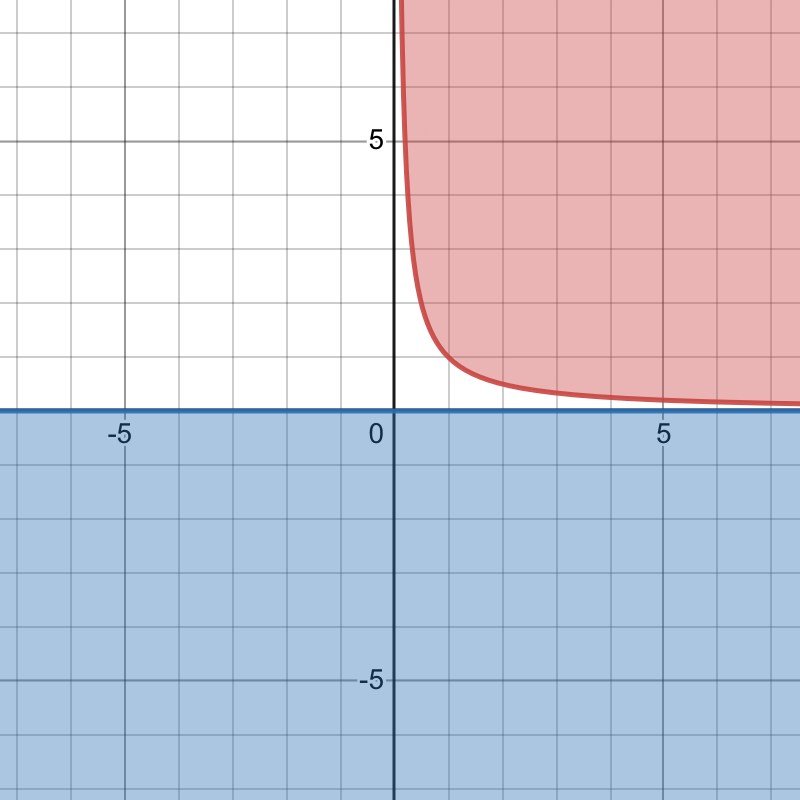
\includegraphics[width=5cm]{Exercise 32.png}
        \caption{Set A (red) and B (blue).}
        \label{fig:my_label}
    \end{figure}
    
    If $(a_n,b_n)\in B$ and $(a_n,b_n)\rightarrow (a,b)$ for all $n\in \N$, then we have $b_n\rightarrow b$. Since $b_n\geq 0$ for all $n\in\N$, we must have $b\geq 0$. Therefore, $(a,b)\in B$, which implies $B$ to be a closed set.
    
    Similarly, for any $(a,b)\in \R^2$, if $(a_n,b_n)\in A$ and $(a_n,b_n)\rightarrow (a,b)$ for all $n\in\N$, then $a_n\rightarrow a$ and $b_n\rightarrow b$. We will now prove that $a\neq 0$, thus $\frac{1}{a_n}\rightarrow\frac{1}{a}$. Indeed, because $b_n\rightarrow b>0$, there exists $\delta>0$ such that $b_n$ will eventually in $(b-\delta, b+\delta)$. Thus $b_n$ will eventually smaller than $b+\delta$. That is when $n$ is big enough, because $b_n\geq \frac{1}{a_n}$, we get 
    \[
    a_n\geq \frac{1}{b_n}\geq \frac{1}{b+\delta}.
    \]
    Since $a_n\rightarrow a$, we also get 
    \[
    a\geq \frac{1}{b+\delta}>0.
    \]
    Hence $\frac{1}{a_n}\rightarrow\frac{1}{a}$.
    
    We then prove that $b\geq \frac{1}{a}$ too. Indeed, if $b<\frac{1}{a}$, then there exists $\epsilon>0$ such that $b-\frac{1}{a}<-\epsilon<0$. Because $b_n\rightarrow b$ and $\frac{1}{a_n}\rightarrow\frac{1}{a}$, there exists $n_0$ big enough such that $|b_{n_0}-b|<\frac{\epsilon}{2}$ and $|\frac{1}{a}-\frac{1}{a_{n_0}}|<\frac{\epsilon}{2}$. Thus $b_{n_0}-b<\frac{\epsilon}{2}$ and $\frac{1}{a}-\frac{1}{a_{n_0}}<\frac{\epsilon}{2}$. But then we get a contradiction because
    \[
    b_{n_0}-\frac{1}{a_{n_0}}=(b_{n_0}-b)+\left(b-\frac{1}{a}\right)+\left(\frac{1}{a}-\frac{1}{a_{n_0}}\right)<\frac{\epsilon}{2}-\epsilon+\frac{\epsilon}{2}=0
    \]
    and $(a_{n_0},b_{n_0})\in A$ so $b_{n_0}-\frac{1}{a_{n_0}}\geq0$. Therefore, $A$ is also a closed set. Since it's pretty clear that $A\cap B=\varnothing$, it's sufficient to prove that $d(A,B)=0$. Indeed, let $x_n=(n,\frac{1}{n})\in A$ and $y_n=(n,0)\in B$ for all $n\in\N$, we have
    \begin{align*}
        0&\leq \inf\{d(a,b):a\in A,b\in B\}\\
        &\leq \inf\{d(x_n,y_n):n\in \N\}\\
        &=\inf\{\frac{1}{n}:n\in\N\}\\
        &= 0.
    \end{align*}
    Hence, $A$ and $B$ are two disjoint closed set and $d(A,B)=0$.
    \end{proof}

33.
\begin{proof}
Assume that $x$ is a limit point, for any $\epsilon>0$, we will prove that $B_\epsilon(x)$ has infinite number of points. Indeed, because $x$ is a limit point, there exists $x_1\in B_\epsilon(x)\setminus \{x\}$. Let $0<\epsilon_1<d(x_1,x)$, then because $x_1\in B_\epsilon(x)$, we get $\epsilon_1<d(x_1,x)<\epsilon$. Thus $B_{\epsilon_1}(x)\subset B_\epsilon(x)$ and $x_1\notin B_{\epsilon_1}(x)$. Therefore, there exists $x_2\neq x_1$ such that $x_2\in B_{\epsilon_1}(x)\setminus \{x\}$. In general, if $x_n\in B_{\epsilon_{n-1}}(x)$, define $0<\epsilon_n<d(x_n,x)<\epsilon_{n-1}$.  Then $x_k\notin B_{\epsilon_{n}}(x)$ for all $k=1,\cdots ,n$ because
\[
\epsilon_n<d(x_n,x)<\epsilon_{n-1}<d(x_{n-1},x)<\cdots <d(x_1,x).
\]
Since $x$ is a limit point, let $x_{n+1}\in B_{\epsilon_n}(x)\setminus \{x\}$. So, we have construct a sequence of distinct elements $x_n$ and $x_n\in B_\epsilon(x)$ for all $n\in\N$. Therefore, every neighborhood of $x$ contains infinitely many points of $A$.
\end{proof}

34.
\begin{proof}
If $x$ is a limit point, then $B_\frac{1}{n}(x)\setminus\{x\}$ is nonempty for all $n\in\N$. Therefore, let $x_n\in B_\frac{1}{n}(x)\setminus\{x\}$. Because $\frac{1}{n}\rightarrow 0$, we get $x_n\rightarrow x$ and $x_n\neq x$ for all $n\in\N$. If there exists a sequence $x_n\rightarrow x$ and $x_n\neq x$ for all $x$, then for any $\epsilon>0$, by the definition of convergence, $x_n$ will eventually in $B_\epsilon(x)$. Therefore, $B_\epsilon(x)\setminus\{x\}\neq \varnothing$, which means $x$ is a limit point.
\end{proof}

36.
\begin{proof}
Let $a_n\in A$ and $a_n\rightarrow a$, we will prove that $a\in A$. If $a=x$, then done. If $a\neq x$, let $0<\epsilon <d(a,x)$. Because $x_n\rightarrow x$, we get $x_n\in B_\epsilon(x)$ for all but finitely many points. Let $0<\delta<d(a,x)-\epsilon$, then $\delta +\epsilon<d(a,x)$, which implies $B_\epsilon(x)$ and $B_\delta(a)$ are distinct. That is $B_\epsilon(x)\cap B_\delta(a)=\varnothing$. Therefore, $\{a_n:a_n\in B_\delta(a)\}$ has finitely many distinct values, which means there exists $m=\min\{d(a_n,a):a_n\in B_\delta(a), d(a_n,a)>0\}$. Then $B_m(a)$ has only elements equal $a_n$, which implies $a=a_k=x_h$ for some $k,h\in\N$. Therefore, $a\in A$. We get $A$ is a closed set.
\end{proof}

\pagebreak

40.
\begin{proof}
By definition, $x$ is a limit point if for all $\epsilon >0$, we have $(B_\epsilon(x)\setminus \{x\})\cap A\neq\varnothing$.  Therefore, $x$ is \textbf{not} a limit point if there exists $\epsilon>0$ such that $(B_\epsilon(x)\setminus \{x\})\cap A=\varnothing$.    

Let $A\subset \R$, we need to prove that $A$ has at most countably many isolated points. For any isolated point $a$ in $A$, by the definition, there exists $\epsilon_a$ such that $(B_{2\epsilon_a}(a)\setminus\{a\})\cap A=\varnothing$. Then for any  two isolated point $a,b$ in A, we will claim that $B_{\epsilon_a}(a)\cap B_{\epsilon_b}(b)=\varnothing$. Indeed, if $k\in B_{\epsilon_a}(a)\cap B_{\epsilon_b}(b)$, then 
\[
d(a,b)\leq d(a,k)+d(k,b)<\epsilon_a +\epsilon_b <2\max\{\epsilon_a,\epsilon_b\}.
\]
Without loss of generality, assume that $\max\{\epsilon_a,\epsilon_b\}=\epsilon_a$, then the equation above gives $d(a,b)<2\epsilon_a$, which implies $b\in B_{2\epsilon_a}(a)$, contradiction. Therefore, $B_{\epsilon_a}(a)\cap B_{\epsilon_b}(b)=\varnothing$ for any isolated points $a,b\in A$. Now, let $f$ be a function map the set of isolated points in $A$ to distinct intervals in $\R$, namely $f(a)=B_{\epsilon_a}(a)$. Because these intervals are distinct, $f$ is an injection. Moreover, the set of open intervals of $\R$ is countable, therefore, the set of isolated points of $A$ is also countable.
\end{proof}

41.
\begin{proof}
\hfill
\begin{enumerate}[label=(\alph*)]
\item If $x\in bdry(A)$, then by the definition, for any $\epsilon>0$, we have $B_\epsilon(x)\cap A=\varnothing$ and $B_\epsilon(x)\cap A^c=\varnothing$. Notice that $A=(A^c)^c$, thus $B_\epsilon(x)\cap (A^c)^c=\varnothing$. Therefore, $x\in bdry(A^c)$ too. Similarly, if $x\in bdry(A^c)$, then for any $\epsilon>0$, we have $B_\epsilon	(x)\cap A^c=\varnothing$ and $B_\epsilon(x)\cap A= B_\epsilon(x)\cap (A^c)^c=\varnothing$. Therefore $x\in bdry (A)$, which means $bdry(A)=bdry(A^c)$. 

\item Assume that $x\in cl(A)$, we need to prove that $x\in bdry(A)\cup int(A)$. Indeed, if $x\in int(A)$, then we are done. If $x\notin int(A)$, then by the definition, for any $\epsilon>0$, we have $B_\epsilon(x)\not\subset A$. That is $B_\epsilon(x)\cap A^c\neq \varnothing$. Moreover, because $x\in cl(A)$, for any $\epsilon>0$, we have $B_\epsilon(x)\cap A\neq \varnothing$. Therefore, $x\in bdry(A)$. So $x\in cl(A)$ implies $x\in bdry(A)\cup int(A)$. Conversely, assume that $x\in bdry(A)\cup int(A)$. If $x\in bdry(A)$, then by the definition, $B_\epsilon(x)\cap A\neq \varnothing$ for all $\epsilon>0$. Therefore, $x\in cl(A)$. If $x\notin bdry(A)$, then $x\in int(A)\subset A\subset cl(A)$. Therefore, $x\in bdry(A)\cup int(A)$ implies $x\in cl(A)$. Thus $cl(A)=bdry(A)\cup int(A)$.

\item We need to prove that $M=cl(A)\cup int(A^c)$, thus by part (b), we get $M=bdry(A)\cup int(A)\cup int(A^c)$. Indeed, for any $x\in M$, assume that $x\notin int(A^c)$. Notice that by definition, $x\in int(A^c)$ means there exists $\epsilon>0$ such that $B_\epsilon(x)\subset A^c$, that is $B_\epsilon(x)\cap A=\varnothing$. Therefore, $x\notin int(A^c)$ means for any $\epsilon>0$, $B_\epsilon(x)\cap A\neq \varnothing$. Thus $x\in cl(A)$. So $M=cl(A)\cup int(A^c)=bdry(A)\cup int(A)\cup int(A^c)$.
\end{enumerate}
\end{proof}

\pagebreak 

46.
\begin{proof}
The proof is by showing that $A$ is dense in $M$ implies (a), (a) implies (b), (b) implies (c), (c) implies (d), and finally (d) implies $A$ is dense in $M$.
\hfill
\begin{enumerate}[label=(\roman*)]
\item If $A$ is dense in $M$, by the definition, we have $\overline{A}=M$. Therefore, for any $x\in M$, we get $x\in \overline{A}$. Therefore, there exist $a_n\in A$ such that $a_n\rightarrow x$.

\item Assume that every point in $M$ is a limit of a sequence from $A$, then for any $x\in M$, there exists $a_n\in A$ and $a_n\rightarrow M$. That is, for any $\epsilon>0$, $a_n$ will eventually in $B_\epsilon(x)$. Therefore, $B_\epsilon(x)\cap A\neq \varnothing$ for every $x\in M$ and $\epsilon>0$.

\item Assume that (b) holds. For any open set $U$, if $U=\varnothing$, then obviously $U\cap A=\varnothing\cap A=\varnothing$. If $U\neq \varnothing$, then there exists $x\in U$. Because $U$ is an open set, there exists $\epsilon>0$ such that $B_\epsilon(x)\subset U$. But by (b), $B_\epsilon(x)\cap A\neq \varnothing$, therefore, $U\cap A\neq \varnothing$.

\item Assume that (c) holds and $int(A^c)$ is not empty, then there exists $x\in int(A^c)$. Because $int(A^c)$ is an open set, there exists $\epsilon>0$ such that $B_\epsilon(x) \subset int(A^c)\subset A^c$. Thus $B_\epsilon(x)\cap A=\varnothing$, which is contradicting to (c). So (c) implies $A^c$ is empty interior.

\item Assume that (d) holds, in exercise 41.c, we have proved that for any $A\subset M$, $M=cl(A)\cup int(A^c)$. But $int(A^c)=\varnothing$, therefore, $M=cl(A)=\overline{A}$. Thus by the definition, $A$ is dense in $M$. 
\end{enumerate}
\end{proof}

48.
\begin{proof}
We will show that $\Q^n$ is dense in $\R^n$ for any $n\in \N$. Indeed, for any $r=(r_1,\cdots ,r_n)\in R_n$, because $\Q$ is dense in $\R$, there exists $q_i^{(k)}\in \Q$ such that $q_i^{(k)}\rightarrow r_i$. Therefore, $q_k=(q_1^{(k)},\cdots ,q_n^{(k)})\in \Q^n$ and $q_k\rightarrow r$. By (a) exercise 46, $\Q^n$ is dense in $\R^n$. Because $\Q^n$ is countable, $\R^n$ is separable for any $n\in\N$. Thus both $\R$ and $\R^2$ are separable.
\end{proof}

\pagebreak

49.
\begin{proof}
Let $R$ be the set of sequences of the form $(r_1,\cdots ,r_n,0,0,\cdots )$, where each $r_k$ is rational. That is $R=\{r=(r_1,\cdots ,r_n,0,0,\cdots ): n\in\N, r_i\in\Q \text{ for all } i\in \N\}$. We will prove that $R$ is dense in $\ell_2$ by showing that for any $x\in \ell_2$ and $\epsilon>0$, $B_\epsilon(x)\cap R\neq \varnothing$. Let $x=(x_1,x_2,\cdots)$, because $x\in \ell_2$, we have $\sum_{i=1}^{\infty}{x_i^2}<\infty$. That is, for some $N\in\N$ big enough, we have
\[
\left|\sum_{i=1}^{\infty}{x_i^2} -\sum_{i=1}^{N}{x_i^2}\right|<\frac{\epsilon^2}{2}\quad \text{ or } \quad \sum_{i=N+1}^{\infty}{x_i^2}<\frac{\epsilon^2}{2}.
\] 
Now all we need to do is to choose $(r_1,\cdots ,r_n,0,\cdots)\in R$ such that $\sum_{n=1}^{N}{(x_i-r_i)^2}<\frac{\epsilon^2}{2}$, then
\begin{align*}
\|x-r\|_2&=\|(x_1-r_1,\cdots, x_n-r_n, x_{n+1},\cdots)\|_2\\
&=\left(\sum_{i=1}^{N}{(x_i-r_i)^2}+\sum_{i=N+1}^{\infty}{x_i^2}\right)^\frac{1}{2}\\
&\leq \left(\frac{\epsilon^2}{2}+\frac{\epsilon^2}{2}\right)^\frac{1}{2}\\
&=\epsilon.
\end{align*}
That is $r\in B_\epsilon(x)$, so $B_\epsilon(x)\neq \varnothing$. But the selection of $r_i$'s is not hard. By the density of $\Q$ in $\R$, for any $x_i$, there exists an $r_i\in \Q$ such that $x_i-\frac{\epsilon}{\sqrt{2N}}<r_i<x_i$ for all $i\in \N, i\leq N$. Therefore, $0<x_i-r_i<\frac{\epsilon}{\sqrt{2N}}$, which implies $(x_i-r_i)^2<\frac{\epsilon^2}{2N}$ for all $i$. Hence
\[
\sum_{i=1}^{N}{(x_i-r_i)^2}<N\cdot \frac{\epsilon^2}{2N}=\frac{\epsilon^2}{2}.
\]

Now we will prove that $R$ is countable. Because $card(\Q)=card(\N)$, let $N=\{(n_1,\cdots ,n_k,0,\cdots):n_i,k\in\N \text{ for all } i\in \N\}$, then $N\sim R$. Rearrange $N$ into this order:
\[
(1,0,\cdots),(1,1,0,\cdots),(2,0,\cdots),(1,1,1,0,\cdots),(1,2,0,\cdots),(2,1,0,\cdots),(3,0,\cdots),\cdots
\]
where every element is increasing by the sum of all entries and increasing by the entries by left to right. It's not hard to see that $N$ is countable, therefore $R$ is countable. 

Similar for $H^\infty$, let us define $S=\{(r_1,\cdots,r_n,0,\cdots):n\in\N, r_i \text{ is rational and } 0\leq r_i\leq 1\}$. Because $S\subset R$, we get $S$ is countable as well. Now we will prove that $S$ is dense in $H^\infty$. For any $x\in H^\infty$ and $\epsilon>0$, we will show that $B_\epsilon(x)\cap R\neq \varnothing$. Because $\sum_{n=1}^{\infty}{2^{-i}}$ is converges, there exists $N\in\N$ such that 
\[
\sum_{i=N+1}^{\infty}{2^{-i}}<\frac{\epsilon}{2}.
\]
Then because $|x_i|<1$ for any $i\in\N$, we get
\[
\sum_{i=N+1}^{\infty}{2^{-i}|x_i-0|}\leq \sum_{i=N+1}^{\infty}{2^{-i}}<\frac{\epsilon}{2}.
\]
Let $r_1,\cdots ,r_N$ be rational numbers in $[0,1]$ such that $|x_i-r_i|<\frac{\epsilon}{2N}$ for any $1\leq i\leq N$. Such $r_i$ exists because $x_i\in [0,1]$ too, so by the density of $\Q$ in $\R$, $|x_i-r_i|$ can be as small as possible. Then we have $s=(r_1,\cdots,r_N,0,\cdots)\in S$ and
\[
\sum_{i=1}^{N}{2^{-i}|x_i-r_i|}\leq \sum_{i=1}^{N}{|x_i-r_i|}\leq N\cdot \frac{\epsilon}{2N}=\frac{\epsilon}{2}.
\]
Therefore, 
\begin{align*}
d(x,s)&=\sum_{i=1}^{\infty}{2^{-i}|x_i-r_i|}\\
&=\sum_{i=1}^{N}{2^{-i}|x_i-r_i|}+\sum_{i=N+1}^{\infty}{2^{-i}|x_i|}\\
&\leq \frac{\epsilon}{2}+\frac{\epsilon}{2}\\
&=\epsilon.
\end{align*}
That is $s\in B_\epsilon(x)\cap S\neq \varnothing$. So $H^\infty$ is separable.
\end{proof}

50.
\begin{proof}
Let $S$ be the set of sequences of $0$'s and $1$'s, then in chapter 3, we know that $S$ is uncountable. For any set $A$ a subset of $\ell_\infty$ and $A$ is dense in $\ell_\infty$, we will prove that $card(A)$ is at least $card(S)$, thus $A$ is uncountable. Let $0<\epsilon<\frac{1}{2}$, we will claim that for any $a,b\in S$ and $a\neq b$, $B_\epsilon(a)\cap B_\epsilon(b)=\varnothing$. Indeed, assume that $k\in B_\epsilon(a)\cap B_\epsilon(b)$, let $a_i,b_i,k_i$ be the $i$th element of the sequence $a,b,k$ respectively. Because $a\neq b$, there exists $i\in \N$ such that $a_i\neq b_i$. Thus
\[
1= d(a_i,b_i)\leq d(a_i,k_i)+d(k_i,b_i)<\epsilon +\epsilon<\frac{1}{2}+\frac{1}{2}=1,
\]
contradiction. Therefore, $B_\epsilon(a)\cap B_\epsilon(b)=\varnothing$. Notice that because $A$ is dense in $\ell_\infty$, $B_\epsilon(a)\cap A\neq \varnothing$ for any $a\in S$. That is, there is at least one element from $A$ in $B_\epsilon(a)$ for any $a\in S$. Since $B_\epsilon(a)$'s are distinct when $a$ range in $S$, there is a one to one map from $S$ to $A$. Thus $card(S)\leq card(A)$, which implies $A$ is uncountable. Therefore, $\ell_\infty$ is not separable. 
\end{proof}

51.
\begin{proof}
Let $M$ be a separable metric, and $I$ be the set of isolated points of $M$, we need to prove that $I$ is countable. Because $M$ is separable, there exists a countable set $A$ such that $A$ is dense in $M$. For any $x\in I$, because $x$ is an isolated point, there exists $\epsilon>0$ such that $(B_\epsilon(x)\setminus\{x\})\cap M=\varnothing$. Since $A\subset M$, we get $(B_\epsilon(x)\setminus\{x\})\cap A=\varnothing$. But $A$ is dense in $M$, therefore, $B_\epsilon(x)\cap A\neq \varnothing$. That is $x\in A$. So $I\subset A$. Since $A$ is countable, $I$ is also countable.
\end{proof}

61.
\begin{proof}
\hfill
\begin{enumerate}
\item[(ii)] Assume that $F=A\cap C$ where $C$ is closed in $(M,d)$. For any $x\in A$ such that $B_{\epsilon}^A(x)\cap F\neq \varnothing$ for all $\epsilon>0$, we will prove that $x\in F$. Indeed, since $B_\epsilon^A(x)\subset B_\epsilon^M(x)$ and $F\subset C$, $B_{\epsilon}^A(x)\cap F\neq \varnothing$ implies $B_\epsilon^M(x)\cap C\neq \varnothing$ for all $\epsilon>0$. Because $C$ is a closed set, by the definition, we get $x\in C$. Notice that $x\in A$, thus $x\in A\cap C=F$.

Conversely, if $F$ is a closed set in $A$, we will prove that $F=cl_M(F)\cap A$, thus $cl_M(F)$ is the closed set that we are looking for. Since $F\subset cl_M(F)$ and $F\subset A$, we get $F\subset cl_M(F)\cap A$. For any $x\in cl_M(F)\cap A$, by the definition of closure, $B_\epsilon^M(x)\cap F\neq \varnothing$ for all $\epsilon>0$. But $F\subset A$, therefore $B_\epsilon^A(x)\cap F=B_\epsilon^M(x)\cap A\cap F\neq \varnothing$ for all $\epsilon>0$. Because $F$ is a closed set in $A$, we get $x\in F$. That is $cl_M(F)\cap A\subset F$. Therefore, $cl_M(F)\cap A=F$.

\item[(iii)] In the previous part, we have shown that if $F$ is closed in $A$, then $F=cl_M(F)\cap A$. Let $F=cl_A(E)$, then $cl_A(E)=A\cap cl_M(cl_A(E))$. Therefore, it is sufficient to prove that $cl_M(E)=cl_M(cl_A(E))$. Because $E\subset cl_A(E)$, we get $cl_M(E)\subset cl_M(cl_A(E))$. Otherwise, if $x\in cl_M(clA(E))$, then by the definition, $B\epsilon^M(x)\cap clA(E)\neq \varnothing$ for all $\epsilon>0$. Assume that there is $\delta>0$ such that $B{\delta}^M(x)\cap E=\varnothing$, then we will claim that $B_{\delta/2}^M(x)\cap cl_M(E)=\varnothing$. Thus since $cl_A(E)\subset clM(E)$, we get $B{\delta/2}^M(x)\cap clA(E)=\varnothing$. Contradiction! Well indeed, for any $a\in B{\delta/2}^M(x)$, we get $d(a,x)<\frac{\delta}{2}$. And since $B\delta(x)^M\cap E=\varnothing$, we get $d(x,E)>\delta$. Therefore, $d(a,E)>d(x,E)-d(a,x)>\delta-\frac{\delta}{2}=\frac{\delta}{2}$. Hence $B{\delta/2}^M(a)\cap E=\varnothing$, which implies $a\notin clM(E)$. So $B{\delta/2}^M(x)\cap clM(E)=\varnothing$, which implies $B\delta^M(x)\cap E\neq \varnothing$ for all $\delta>0$. Thus $x\in cl_M(E)$ for any $x\in cl_M(cl_A(E))$, that is $cl_M(cl_A(E))\subset cl_M(E)$. In consumption, $cl_M(cl_A(E))=cl_M(E)$, thus $cl_A(E)=A\cap cl_M(E)$.
\end{enumerate}
\end{proof}

62.
\begin{proof}
If $G$ is open in $M$, then because $G\subset A$, we get $G=A\cap G$. Therefore $G$ is also open in $A$. Conversely, if $G$ is open in $A$, then for any $x\in G\subset A$, there exists $\epsilon>0$ such that $B_\epsilon^M(x)\subset A$. Because $G$ is open in $A$, there exists $0<\delta<\epsilon$ such that $B_\delta^A(x)\subset G$. That is $B_\delta^M(x)\cap A\subset G$. Notice that $B_\delta^M(x)\subset B_\epsilon^M(x)\subset A$, therefore, $B_\delta^M(x)\cap A=B_\delta^m(x)$. Thus $B_\delta^M(x)\in G$ for any $x\in G$. That is $G$ is an open set in $M$.

Replace "open" by "closed", the statement becomes $A$ is closed in $(M,d)$ and $G\subset A$, then $G$ is closed in $A$ if and only if $G$ is closed in $M$. If $G$ is closed in $M$, then because $G=G\cap A$, by exercise 61, we get $G$ is closed in $A$. Conversely, if $G$ is closed in $A$, then for any sequence $x_n\in G\subset A$ and $x_n\rightarrow x$ where $x\in M$, then because $A$ is a closed set in $M$, we get $x\in A$. Moreover, since $G$ is a closed set in $A$, we also get $x\in G$. So by the definition of closed set, $G$ is a closed set in $M$. So the statement still holds.
\end{proof}

63.
\begin{proof}
Let $A$ be a nonempty subset of $\R$, then in $\R^2$, $A=\{(a,0):a\in A\}$. Clearly this is not an open set because let $(a,0)\in A$, then for any $\epsilon>0$, $(a,\epsilon/2)\in B_\epsilon^{\R^2}(a,0)$ but $(a,\epsilon/2)\notin A$. Therefore $B_\epsilon^{\R^2}(a,0)\not\subset A$ for any $\epsilon>0$, which means $A$ is not open.

Let $A=[0,1]$ be a closed set in $\R$, then in $\R^2$, $A=\{(a,0):a\in [0,2]\}$. We will claim that $A$ is a closed set in $\R^2$. Indeed if $(x_n,0)\in A$ and $(x_n,0)\rightarrow (x,y)$ for some $(x,y)\in \R^2$, then we get $x_n\rightarrow x$ and $0\rightarrow y$. Since $A$ is closed in $\R$, we get $x\in A$ in $\R$. Clearly $y=0$, therefore $(x,y)\in A$ in $\R^2$. Thus $A$ is a closed set in $\R^2$.
\end{proof}

64.
\begin{proof}
The analogue of part (iii) gonna be $int_A(E)=A\cap int_M(E)$ for any subset $E$ of $A$. Let $E=A=[0,2]$ in $\R$, then $E$ is an open set in $A$, thus $int_A(E)=[0,2]$, which is not equals $int_\R(E)=(0,2)$.
\end{proof}

69.
\begin{proof}
If $M$ has a countable open base, then let $a$ be a random element in each open base. The set $A$ of such $a$ is therefore countable. Moreover, for any open set $U\in M$, there exists an open set of the open base such that it is a subset of $U$. Thus $U\cap A\neq\varnothing$ for all open set $U$, which means $M$ is separable.

Conversely,if $M$ is separable, then there exists a countable dense subset $\{x_n\}$ of $M$. Let $U=\{B_\epsilon(x_n):\epsilon\in\Q\}$, we will prove that $U$ is a countable open base of $M$. Notice that $\{x_n\}$ and $\{\epsilon\}$ have the same cardinality as $\N$, we get $card(U)=card(\N\times \N)=card(\N)$. Therefore $U$ is countable. For any open set $O$ in $U$, we will claim that $O=\cup\{B_\epsilon(x_n):B_\epsilon(x_n)\in O\cap U\}$. Indeed, since $B_\epsilon(x_n)\subset O$, there union is obviously a subset of $O$. Now, for any $a\in O$, there exists a rational $\delta>0$ such that $B_\delta(a)\subset O$. Since $U$ is dense, there exists $x_k\in B_\frac{\delta}{2}(a)$. Hence $a\in B_\frac{\delta}{2}(x_k)\subset B_\delta(a)\subset O$. (I'm not sure if this is clear yet so please tell me if you want further explanation.) Since $\frac{\delta}{2}$ is rational, we get $B_\frac{\delta}{2}(x_k)\subset U$, thus $a\in B_ \frac{\delta}{2}(x_k)\subset \cup\{B_\epsilon(x_n):B_\epsilon(x_n)\in O\cap U\}$ for all open set $O\subset M$. Thus $U$ is a countable open base of $M$.
\end{proof}

\pagebreak

\section*{Chapter 5. Continuous Functions}

7.
\begin{proof}
\hfill
\begin{enumerate}[label=(\alph*)]
\item Since $(-\infty,a)$ is an open set in $\R$ and $f$ is continuous, we get $f^{-1}(-\infty,a)=\{x:f(x)<a\}$ is an open set. Similarly, we get $\{x:f(x)>a\}$ is an open set.

\item For any $\epsilon>0$, because $B_\epsilon^\R(f(a))=\{f(x):f(a)-\epsilon<f(x)<f(a)+\epsilon\}$, we get $f^{-1}(B_\epsilon^\R(f(a)))=\{x:f(a)-\epsilon<f(x)<f(a)+\epsilon\}$. Notice that $\{x:f(x)<f(a)+\epsilon\}$ and $\{x:f(x)>f(a)-\epsilon\}$ are open by the hypothesis, therefore, their intersection is also open, namely $f^{-1}(B_\epsilon(f(a)))=\{x:f(a)-\epsilon<f(x)<f(a)+\epsilon\}$. Since $a\in f^{-1}(B_\epsilon(f(a)))$ an open set, there exists $\delta>0$ such that $B_\delta^M(a)\subset f^{-1}(B_\epsilon(f(a)))$. Thus $f$ is continuous.

\item Assume that the sets $\{x:f(x)>q\}$ and $\{x:f(x)<q\}$ are open for any $q\in\Q$, let $a\in\R$, we will prove that $\{x:f(x)>a\}$ and $\{x:f(x)<a\}$ are open too. Indeed, for any $y\in\{x:f(x)>a\}$, we have $f(y)>a$, thus there exists $a'\in\Q$ such that $f(y)>a'>a$. (This is by the density of $\Q$ in $\R$.) By the assumption, we get $y\in \{x:f(x)>a'\}$ an open set, therefore, there exists $\delta>0$ such that $B_\delta^M(y)\subset\{x:f(x)>a'\}\subset \{x:f(x)>a\}$. Thus $\{x:f(x)>a\}$ is open, the same implies for $\{x:f(x)>a\}$, thus by part (b), $f$ is continuous.
\end{enumerate}
\end{proof}

10.
\begin{proof}
For any $\epsilon>0$, we have $B_\frac{1}{2}^A(2)=\{f(2)\}\subset f^{-1}(B_\epsilon(f(2)))$. Therefore, $f$ is continuous relative to $A$ at $2$.
\end{proof}

\pagebreak

11.
\begin{proof}
\hfill
\begin{enumerate}[label=(\alph*)]
\item We will prove that this statement is true. For any $a\in A\cup B$, without loss of generality, assume that $a\in A$. Since $f$ is continuous at each point in $A$, we get $f$ to be continuous at $a$ as well. Thus $f$ is continuous at each point of $A\cup B$.

\item Let 
\[
f(x)=\left\{\begin{array}{lr}
0, &\text{ for all } x\in A=(1,2]\\
2, &\text{ for all } x\in B=(2,3)
\end{array}\right..
\]
It's not hard to see that $f$ is continuous relatively to $A$ or $B$. However, for any $\delta>0$, we have $B_\delta(2)=\{2-\delta,2+\delta\}$. But let $\epsilon = 1$, then we get $f^{-1}(B_\epsilon^{A\cup B}(f(2)))=f^{-1}(B_1^{A\cup B}(0))=f^{-1}(0)=(1,2]$. Clearly $B_\delta(2)\not\subset f^{-1}(B_\epsilon^{A\cup B}(f(2)))$, thus $f$ is not continuous relatively to $A\cup B$ at $2$.

The modification that is necessary to make (b) true is that $A$ and $B$ are open in $M$. If so then for any $a\in A\cup B$, then without loss of generality, let $a\in A$. For any $\epsilon>0$, because $f$ is continuous relatively to $A$ at $a$, there exists $\delta>0$ such that $B_\delta^M(a)\cap A=B_\delta^A(a)\subset f^{-1}(B_\epsilon(f(a)))$. Notice that both $B_\delta^M(a)$ and $A$ are open sets, we get $B_\delta^M(a)\cap A$ is an open set. Thus there exists $\gamma>0$ such that $B_\gamma^M(a)\subset B_\delta^M(a)\cap A$. Thus $B_\gamma^{A\cup B}(a)\subset B_\gamma^M(a)\subset B_\delta^M(a)\cap A\subset f^{-1}(B_\epsilon(f(a)))$. That is, $f$ is continuous relative to $A\cup B$.
\end{enumerate}
\end{proof}

14.
\begin{proof}
Let $C$ denote the set of continuous functions $f:\R\rightarrow\R $ and $c=\card(\R)$. Let $R=\{f(x): f\text{ is any function from }\Q\text{ to }\R\}$. Because a continuous function of $\R$ is determined by its values on $\Q$, there is a one to one map from $C$ to $R$, namely the map preserved the value of $f$ at any rational point. Thus $\card(C)\leq \card(R)$.

Let $h:\R\mapsto C$ defined by $h(x)=x$ for all $x\in \R$. It's not hard to see that $h$ is a one to one function, thus $c=\card(\R)\leq \card(C)\leq \card(R)=c^{\aleph_0}=c$. So $\card(C)=c$. 
\end{proof}

17.
\begin{proof}
For any $a\in M$, if $f(a)\neq g(a)$, then we get $\rho (f(a),g(a))>2\epsilon>0$ for some $\epsilon>0$. Because $f$ and $g$ are continuous, there exists $\delta>0$ such that $f(B_\delta^d(a))\subset B_\epsilon^\rho(f(a))$ and $g(B_\delta^d(a))\subset B_\epsilon^\rho(g(a))$. Because $D$ is dense in $M$, there exists $b\in B_\delta^d(a)\cap D$. Then because $b\in B_\delta^d(a)$, we get $f(b)=g(b)\in B_\epsilon^\rho(f(a))\cap B_\epsilon^\rho(g(a))$. But then, we have
\[
2\epsilon < \rho(f(a),g(a)) < \rho(f(a),f(d)) + \rho(g(d),g(a)) < \epsilon+\epsilon.
\]
Contradiction! Therefore $\rho(f(a),g(a))=0$, that is $f(a)=g(a)$ for all $a\in M$.

Now we will prove that if $f$ is onto, then $f(D)$ is dense in $N$. Also notice that all the hypotheses we need are $f$ to be continuous and onto, and $D$ is dense in $M$. This result will be reused in exercise 18. For any nonempty open set $O$ of $N$, we get $f^{-1}(O)$ is an open set in $M$. Because $f$ is onto, $f^{-1}(O)\neq \varnothing$. Since $D$ is dense in $M$, there exists $c\in D\cap f^{-1}(O)$. Then $f(c)\in f(D)\cap O\neq \varnothing$. That is, $f(D)\cap O\neq \varnothing$ for any non empty open set $O$ of $N$. Thus $f(D)$ is dense in $N$.
\end{proof}

18.
\begin{proof}
Because $A$ is separable, there exists a countable dense subset $D$ of $A$. $f(D)$ is clearly countable, it is sufficient to show that $f(D)$ is also dense in $f(A)$. Notice that $f:A\mapsto f(A)$ is onto and continuous, by exercise 17, we get $f(D)$ is dense in $f(A)$. Thus $f(A)$ is also separable.
\end{proof}

20.
\begin{proof}
Because $d$ defines a metric on $M$, we get $d(y,z)\leq d(x,z)+d(x,y)$ and $d(x,z)\leq d(x,y)+d(y,z)$. That is $-d(x,y)\leq d(x,z)-d(y,z)\leq d(x,y)$ or $|d(x,z)-d(y,z)|\leq d(x,y)$.

Now, for any $a\in M$ and $\epsilon>0$, we have $B_\epsilon(f(a))=B_\epsilon(d(a,z))=(d(a,z)-\epsilon,d(a,z)+\epsilon)$. We will prove that for $\delta<\epsilon$, $f(B_\delta(a))\subset B_\epsilon(f(a))$, thus $f$ is continuous. Indeed, for any $x\in B_\delta(a)$, we have $d(x,a)<\delta<\epsilon$. Therefore, by the previous part, we have $d(a,z)-\epsilon<d(a,z)-d(a,x)<d(x,z)$. Moreover, $d(x,z)<d(a,z)+d(x,a)<d(a,z)+\epsilon$. Thus $f(x)=d(x,z)\in (d(a,z)-\epsilon,d(a,z)+\epsilon)=B_\epsilon(f(a))$. Thus $f(B_\delta(a))\subset B_\epsilon(f(a))$, which implies $f$ to be continuous.
\end{proof}

21.
\begin{proof}
If $x\neq y$, then $d(x,y)>0$. Thus there exists $\epsilon>0$ such that $d(x,y)>3\epsilon$. Let $U=B_\epsilon(x)$ and $V=B_\epsilon(y)$, we will claim that $\overline{U}$ and $\overline{V}$ are disjoint. Indeed, Since the close balls radius $\epsilon$ centered at $x$ and $y$ are disjoint, their closures are disjoint too.
\end{proof}

22.
\begin{proof}
For any $m>n\in \N$, we get $E(m)-E(n)=(0,\cdots 0,1,\cdots,1,0\cdots)$ where it $n+1$-th to $m$-th entries are $1$'s, and the rest are $0$'s. Therefore $\|E(m)-E(n)\|_1=m-n$, which implies $E$ preserves distance. So $E$ is an isometry.
\end{proof}

\pagebreak

\begin{lemma}{Cardinality}
$\card(\N\times \R)=\card(\R)$.
\end{lemma}
\begin{proof}
Let $f:\N\times \R\mapsto\R$ defined by $f(n,x)=n+\frac{\arctan(x)}{\pi}$. If there are $(n,x)$ and $(m,y)$ in $\N\times \R$ such that $f(n,x)=f(m,y)$, then 
\[
n+\frac{\arctan(x)}{\pi}=m+\frac{\arctan(y)}{\pi}
\]
or 
\[
n-m=\frac{\arctan(x)-\arctan(y)}{\pi}.
\]
Notice that because $\arctan(x)\in (-\frac{\pi}{2},\frac{\pi}{2})$, we get
\[
|n-m|=\frac{|\arctan(x)-\arctan(y)|}{\pi}\leq \frac{|\arctan(x)|+|-\arctan(y)|}{\pi}<\frac{\pi/2+\pi/2}{\pi}=1.
\]
Therefore, $m=n$, which implies $\frac{\arctan(x)-\arctan(y)}{\pi}=0$. Since $\arctan$ is bijective, we get $x=y$. Thus $(n,x)=(m,y)$, which means $f$ is one to one. Therefore, $\card(\N\times\R)\leq \card(\R)$ (1).

Now let $g:\R\mapsto \N\times \R$ defined by $g(x)=(1,x)$. We can easily see that $g$ is a one to one function, therefore, $\card(\R)\leq \card(\N\times\R)$ (2). From (1) and (2), we get $\card(\R)=\card(\N\times\R)$.
\end{proof}

23.
\begin{proof}
For any $x,y\in c_0$, we have
\[
\|x-y\|_\infty=\sup\{|x_i-y_i|:i\in \N\}=\sup( {|x_i - y_i|~\vert~i\in \mathbb{N}}\cup{0})=\|S(x)-S(y)\|_\infty.
\]
So $S$ preserves distance, which means $f$ is an isometry.
\end{proof}

24.
\begin{proof}
Let $f:\R\mapsto V$ defined by $f(\alpha)=\alpha y$ for all $\alpha\in\R$. If $\|y\|=0$, then $y=0$ and $f(\alpha)=0$ for all $\alpha\in\R$. We can easily see that $f$ in this case is continuous. If $\|y\|>0$, then for any $\epsilon>0$ and $\alpha\in\R$, let $\delta<\frac{\epsilon}{\|y\|}$. Thus for any $b\in B_\delta(\alpha)$, we have $\|f(b)-f(\alpha)\|=\|by-\alpha y\|=|b-\alpha|\|y\|$. Notice that because $b\in B_\delta(\alpha)$, we get $|b-\alpha|<\delta<\frac{\epsilon}{\|y\|}$. Therefore, $\|f(b)-f(\alpha)\|<\epsilon$, which implies $f(b)\in B_\epsilon(f(a))$. So $f(B_\delta(\alpha))\subset B_\epsilon(f(a))$. That is $f$ is continuous.

Let $g:V\mapsto V$ defined by $g(x)=x+y$. For any $\epsilon>0$ and $z\in V$, let $0<\delta<\epsilon$. Then for any $x\in B_\delta(z)$, we get $\|x-z\|<\delta$. Therefore
\[
\|g(x)-g(y)\|=\|(x+y)-(z+y)\|=\|x-z\|<\delta<\epsilon.
\]
That is synonymous with saying $g(x)\in B_\epsilon(g(z))$. Thus $g(B_\delta(z))\subset B_\epsilon(g(z))$, which implies $g$ is continuous.
\end{proof}

\pagebreak

25.
\begin{proof}
For any $\epsilon>0$ and $x\in M$, if $K=0$, then $\rho(f(x),f(y))\leq 0$, thus $f(x)=f(y)$ for all $x,y\in M$. Clearly $f$ in this case is continuous. If $K\neq 0$, then let $0<\delta<\frac{\epsilon}{K}$. Then, for any $y\in B_\delta^d(x)$, we get
\[
\rho(f(x),f(y))\leq Kd(x,y)<K\frac{\epsilon}{K}=\epsilon.
\]
Therefore $f(y)\in B_\epsilon^\rho(f(x))$, which implies $f(B_\delta^d(x))\subset B_\epsilon(f(x))$. Thus $f$ is continuous if $f$ is a Lipschitz mapping.
\end{proof}

26.
\begin{proof}
For any $f,g\in C[a,b]$, because $L:C[a,b]\mapsto \R$, we have
\begin{align*}
|L(f)-L(g)|&= \left|\int_{a}^{b}{(f(t)-g(t))dt}\right|\\
&\leq \int_{a}^{b}{|f(t)-g(t)|dt}\\
&\leq \int_{a}^{b}{d(f,g)dt}\\
&=(b-a)d(f,g)
\end{align*}
because $d(f,g)$ is a constant for fixed $f$ and $g$. Therefore, $L(f)=\int_{a}^{b}{f(t)dt}$ is Lipschitz, that is $L$ is continuous.
\end{proof}

27.
\begin{proof}
For any $x,y\in \ell_\infty$, we have
\[
|f(x)-f(y)|=|x_k-y_k|\leq \|x-y\|_\infty.
\]
Therefore, $f$ is Lipschitz with $K=1$. Thus $f$ is continuous.
\end{proof}

28.
\begin{proof}
The proof is by showing that $g$ is Lipschitz. Let $a=(1,\frac{1}{2},\cdots,\frac{1}{n},\cdots)$, then $\|a\|_2=(\sum_{n=1}^{\infty}{\frac{1}{n^2}})^\frac{1}{2}=(\frac{\pi^2}{6})^\frac{1}{2}=\frac{6\pi}{\sqrt{6}}$. Therefore, $a\in \ell_2$. Now, for any $x,y\in \ell_2$, we have
\[
|g(x)-g(y)|=\left|\sum_{n=1}^{\infty}{\frac{x_n}{n}}-\sum_{n=1}^{\infty}{\frac{y_n}{n}}\right|=\left|\sum_{n=1}^{\infty}{\frac{x_n-y_n}{n}}\right|=\langle{x-y,a}\rangle\leq \|a\|_2\|x-y\|_2
\]
by the Cauchy-Schwarz inequality. Thus $g$ is a $\|a\|_2$-Lipschitz image, which implies $g$ is continuous.
\end{proof}

29.
\begin{proof}
Because $y\in\ell_\infty$, $(y_n)$ is bounded. Let $m=\sup\{|y_n|:n\in\N\}$, then for any $a,b\in \ell_1$, we get
\[
\|h(a)-h(b)\|_1=\|((a_n-b_n)y_n)_{n=1}^\infty\|_1\leq \|(a_n-b_n)_{n=1}^\infty\cdot m\|_1=|m|\cdot \|a-b\|_1.
\]
Thus $h$ is $m$-Lipschitz, which implies $h$ is continuous.
\end{proof}

30.
\begin{proof}
If $f$ is continuous, for any $f(a)\in f(\overline{A})$, since $a\in \overline{A}$, there exist $a_n\in A$ such that $a_n\rightarrow a$. But $f$ is continuous, thus $f(a_n)\rightarrow f(a)$. This implies $f(a)\in \overline{f(A)}$. So $f(\overline{A})\subset \overline{f(A)}$. Moreover, for any $a\in f^{-1}(\inter{B})$, we get $f(a)\in\inter{B}$. Thus there exists $\epsilon>0$ such that $B_\epsilon^\rho(f(a))\subset B$. But $f$ is continuous, thus there exists $\delta>0$ such that $B_\delta^d(a)\subset f^{-1}(B_\epsilon^\rho(f(a)))\subset f^{-1}(B)$. So $a\in \inter{(f^{-1}(B))}$ for all $a\in f^{-1}(\inter{B})$, which implies $f^{-1}(\inter{B})\subset \inter{(f^{-1}(B))}$.

If $f(\overline{A})\subset\overline{f(A)}$ for all $A\subset M$, then we will prove that $B$ closed in $N$ will imply $f^{-1}(B)$ closed in $M$. Indeed, if $f^{-1}(B)$ is not closed, then there exists $a\in \overline{f^{-1}(B)}\setminus f^{-1}(B)$. Since $a\in \overline{f^{-1}(B)}$, by the hypothesis, we get 
\[
f(a)\in f(\overline{f^{-1}(B)})\subset \overline{f(f^{-1}(B))}\subset\overline{B}=B.
\]
However, because $a\notin f^{-1}(B)$, we get $f(a)\notin B$. Contradiction. Thus $f^{-1}(B)$ is closed in $M$ whenever $B$ is closed in $N$, which is synonymous with $f$ being continuous. 

Similarly, assume that $f^{-1}(\inter{B})\subset \inter{(f^{-1}(B))}$ for all $B\subset N$, we will prove that $B$ open in $N$ will imply $f^{-1}(B)$ open in $M$. Indeed, if $f^{-1}(B)$ is not open, then there exists $a\in f^{-1}(B)\setminus\inter{(f^{-1}(B))}$. Because $a\notin \inter{(f^{-1}(B))}$, using the hypothesis, we get $a\notin f^{-1}(\inter{B})$ too, which is contradict to the definition of $a$. Therefore $f^{-1}(B)$ must be open in $M$ whenever $B$ is open in $N$, which is synonymous with $f$ is continuous.

So $f$ is continuous if and only if $f(\overline{A})\subset \overline{f(A)}$ for every $A\subset M$ if and only if $f^{-1}(\inter{B})\subset \inter{(f^{-1}(B))}$ for every $B\subset N$.

One example such that $f(\overline{A})\neq \overline{f(A)}$ is let $f:\Q\mapsto \R$ defined by $f(x)=x$ and $A=\Q$. It's not hard to see that this map is 1-Lipschitz, therefore $f$ is continuous. However $f(\overline{A})=f(\Q)=\Q$, which does not equal $\overline{f(A)}=\overline{\Q}=\R$ since $\Q$ is dense in $\R$.
\end{proof}

\pagebreak

31.
\begin{proof}
\hfill
\begin{enumerate}[label=(\roman*)]
\item For any $\epsilon>0$ and $a\in M$, there exists $n\in \N$ such that $a\in U_n$. Since $U_n$ is open, there exists $\gamma>0$ such that $B_\gamma^d(a)\in U_n$. And because $f$ is continuous on $U_n$, there exists $0<\delta<\gamma$ such that $d(a,b)<\delta$ implies $\rho(f(a),f(b))<\epsilon$ for all $b\in M$. Thus $f$ is continuous on $M$.

\item For any $\epsilon>0$ and $a\in M$, since $M$ is a union of a finite number of $E_n$, $a$ is in some finite number of closed sets. Without loss of generality, assume that $a\in E_i$ for all $1\leq i\leq k$ where $k$ is fixed in $\N$. Because $f$ is continuous on each $E_i$, there exists $\delta_i>0$ such that $d(a,b)<\delta_i$ implies $\rho(f(a),f(b))<\epsilon$ for any $b\in E_i$ and for each $1\leq i\leq k$. Now let 
\[
0<\delta<\min(\{\delta_i:1\leq i\leq k\}\cup \{d(a, E_i):k+1\leq i\leq n\}).
\]
Then for any $b\in M$ and $d(a,b)<\delta$ implies $b\in \cup_{i=1}^{k}E_i$. And since $\delta<\delta_i$ for any $i$, we get $\rho(f(a),f(b))<\epsilon$. That is, there exists $\delta>0$ such that $d(a,b)<\delta$ implies $\rho(f(a),f(b))<\epsilon$ for any $\epsilon>0$ and $a\in M$. Thus $f$ is continuous on $M$.

\item Let $f:[0,1]\mapsto \R$ defined by
\[
f(x)=\left\{\begin{array}{lr}
0, & \text{ for } x=0\\
1, & \text{ for } x\in (0,1]
\end{array}\right. .
\]
Clearly $f$ is not continuous on $[0,1]$. However, let $E_1=\{0\}$, $E_n=[\frac{1}{n},1]$ for $n>1$, then $E_i$ is closed for each $i\in\N$. Also, one can easily see that $f$ is continuous on each $E_i$. However, since $\cup_{n=1}^{\infty}{E_n}=[0,1]$, $f$ is not continuous on their union. 
\end{enumerate}
\end{proof}

34.
\begin{proof}
Let $(x_n,y_n)\rightarrow (x,y)$ in $M\times M$, it is sufficient to show that $d(x_n,y_n)\rightarrow (x,y)$. By exercise 3.46, for any metric on $M\times M$, $(x_n,y_n)\rightarrow (x,y)$ implies $x_n\rightarrow x$ and $y_n\rightarrow y$. Therefore, $d(x_n,y_n)\rightarrow d(x,y)$.
\end{proof}

35.
\begin{proof}
If $f:M\rightarrow\R$ is continuous and $V$ is an open set in $\R$, then $f^{-1}(V)=U$ is also open. Conversely, if $U$ is an open set in $M$, then $N=U^c$ is closed in $M$. Let $f:M\rightarrow \R$ defined by $f(x)=d(x,N)$, then $f$ is continuous. Notice that $N$ is closed, we get $f^{-1}(0)=N$. Thus $f^{-1}(\R\setminus\{0\})=M\setminus N=U$. So $\R\setminus\{0\}$ is the open set that satisfy the exercise's conditions. 
\end{proof}

36.
\begin{proof}
If $f(a_n)\rightarrow f(a)$ for every continuous real-value function, then because $f:M\rightarrow\R$ defined by $f(x)=d(a,x)$ is continuous, we get $d(a_n,a)\rightarrow d(a,a)=0$. Therefore, $a_n\rightarrow a$.
\end{proof}

39.
\begin{proof}
Let $U$ be an open set in $M$, and let $U_n=\{x\in M:d(x,U^c)\geq \frac{1}{n}\}$. We will claim that $U_n$'s are closed and $U=\cup_{n=1}^{\infty}{U_n}$; then $U$ can be written as a union of countably many closed set. Indeed, for any fixed $n\in\N$, let $x_n,x\in U_n$ such that $x_n\rightarrow x$. If $d(x,U^c)<\frac{1}{n}$, then there exists $\epsilon>0$ such that $d(x,U^c)<\frac{1}{n}+\epsilon$. Because $x_n\rightarrow x$, there exists $k\in\N$ such that $d(x_k,x)<\epsilon$. But then we have
\[
\frac{1}{n}<d(x_k,U^c)\leq d(x,x_k)+d(x,U^c)<\epsilon +d(x,U^c)<\frac{1}{n},
\]
contradiction!. Therefore $d(x,U^c)\geq \frac{1}{n}$, which means $x\in U_n$ too. Thus $U_n$ is closed for any $n\in\N$. 

Moreover, for any $n\in \N$, if $a\in U_n$, then $d(a,U^c)\geq \frac{1}{n}>0$, which implies $a\notin U^c$ or $a\in U$. Thus $U_n\subset U$ for any $n\in\N$, which implies $\cup_{n=1}^{\infty}U_n\subset U$ (1). For any $a\in U$, because $U$ is open, there exists $\epsilon>\frac{1}{n}>0$ such that $B_\epsilon(a)\subset U$. Therefore, $B_\epsilon(a)\cap U^c=\varnothing$ or $d(a,U^c)>\epsilon>\frac{1}{n}$. This implies $a\in U_n\subset \cup_{n=1}^{\infty}U_n$. Thus $U\subset \cup_{n=1}^{\infty}U_n$ (2). From (1) and (2), we get $U=\cup_{n=1}^{\infty}U_n$.

Similarly, for any closed set $E$ in $M$, let $E_n=\{x\in M:d(x,E)<\frac{1}{n}\}$ be open sets in $M$, then $E=\cap_{n=1}^{\infty}E_n$. Thus every closed set is the intersection of countably many open sets.
\end{proof}

41.
\begin{proof}
For any $x\notin C$, we defined $a_x$ and $b_x$ be the largest number that is smaller than $x$ and the smallest number that is larger than $x$ respectively. If such $\min$ or $\max$ doesn't exists, then $a_n$ and $b_n$ equal $0$. Specifically, $a_x=\max\{a\in C: a<x\}$ and $b_x=\min\{b\in C:x<b\}$ if $\{a\in C: a<x\}$ and $\{b\in C:x<b\}$ are not $\varnothing$. Otherwise, $a_n=b_n=0$. Notice that $\min$ and $\max$ exists because $C$ is closed. We will defined $g(x):\R\rightarrow\R$ by
\[
g(x)=\left\{\begin{array}{lr}
f(x),\quad \text{ for } x\in C\\
(f(b_x)-f(a_x))(x-a_x)+f(a_x),\quad \text{ for } x\in\R\setminus C
\end{array}\right..
\]
Notice that $g(x)$ simply "connect the boundary points" of $C$, one can easily see this function is continuous. Indeed, if $a\in C^o$, then $g(a)$ is continuous. If $a\in\R\setminus C$, then $g(a)$ is also continuous since $\R\setminus C$ is open. Lastly, assume that $a$ is a boundary point of $C$, if the right limit of $g(a)$ is defined by $f$, then $g(a)$ is continuous since $g(a)=f(a)=\lim_{x\rightarrow a^+}f(x)=\lim_{x\rightarrow a^+}g(x)$. If it is defined by $(f(b_x)-f(a_x))(x-a_x)+f(a_x)$, then $a=a_x$ for any $x$ closed enough to $a$. Therefore 
\[
g(a)=g(a_n)=f(a_n)=\lim_{x\rightarrow a_n^+}(f(b_x)-f(a_x))(x-a_x)+f(a_x)=\lim_{x\rightarrow a_n^+}g(x).
\]
Hence $g(x)$ is a continuous function where $g(x)=f(x)$ for any $x\in C$.
\end{proof}

43.
\begin{proof}
By the definition, $d$ and $\rho$ are equivalent means $x_n\xrightarrow{d}x$ if and only if $x_n\xrightarrow{\rho} x$. Therefore, by theorem 5.5, the identity map $i:(M,d)\mapsto (M,\rho)$ is a homeomorphism.
\end{proof}

44.
\begin{proof}
Let $(M,d), (N,\rho), (A,h)$ be metric spaces. Obviously $(M,d)$ is homeomorphic to itself. By theorem 5.5, we know that if $(M,d)$ is homeomorphic to $(N,\rho)$, then $(M,d)$ is homeomorphic to $(N,\rho)$. Now if $(M,d)$ is homeomorphic to $(N,\rho)$, then there exists a homeomorphism $f:(M,d)\mapsto (N,\rho)$. Similarly, if $(N,\rho)$ is homeomorphic to $(A,h)$, then there exists a homeomorphism $g:(N,\rho)\mapsto (A,h)$. We will claim that $g\circ f$ is a homeomorphism from $(M,d)$ to $(A,h)$. Indeed, because both $f$ and $g$ are one to one and onto, we get $g\circ f$ is one to one and onto. Moreover, we have 
\[
x_n\xrightarrow{d} x \text{ if and only if } f(x_n)\xrightarrow{\rho} f(x) \text{ if and only if }g(f(x_n))\xrightarrow{h} g(f(x)).
\]
Thus by theorem 5.5, we have $g\circ f$ is a homeomorphism from $(M,d)$ to $(A,h)$. Thus $(M,d)$ is homeomorphic to $(A,h)$. So "is homeomorphic to" is an equivalent relation.
\end{proof}

45.
\begin{proof}
Let $\N^{-1}=\{(1/n):n\geq 1\}$ and $f:\N\mapsto \N^{-1}$ defined by $f(n)=\frac{1}{n}$. We will prove that $f$ is a homeomophism. For any $a_n,a\in \N$, if $a_n\rightarrow a$, then $a_n$ is eventually equals $a$. Therefore $f(a_n)=\frac{1}{a_n}\rightarrow \frac{1}{a}=f(a)$. Conversely, for any $\frac{1}{a}\in \N^{-1}$, if $\frac{1}{a_n}\rightarrow \frac{1}{a}$ then $\frac{1}{a_n}$ is eventually equal $\frac{1}{a}$ (notice that $0\notin \N^{-1}$. Therefore $a_n$ will eventually equal $a$, or $a_n\rightarrow a$. By theorem 5.5, $f$ is a homeomorphism, which imply $\N$ is homeomorphic to $\N^{-1}$.
\end{proof}

\pagebreak

46.
\begin{lemma}2
If $(M,d)$ is a metric space, then $k(a,b)=\arctan(d(a,b))$ for any $a,b\in M$ defines a metric on $M$.
\end{lemma}
\begin{proof}
Because $d(a,b)\geq 0$ for all $a,b\in M$ we have $k(a,b)=\arctan(d(a,b))\geq 0$ for all $a,b\in M$. If $k(a,b)=0$, then we get $\arctan(d(a,b))=0$. Therefore $d(a,b)=0$, which implies $a=b$. And obviously $k(a,a)=\arctan(d(a,a))=\arctan(0)=0$. Thus $a=b$ in $M$ if and only if $k(a,b)=0$. Also because $k(a,b)=\arctan(d(a,b))=\arctan(d(b,a))=k(b,a)$, if $k$ satisfy the triangular inequality, $k$ defines a metric on $M$. 

For any $a,b\geq 0$, we have $1-ab<1$. Thus
\[
a+b\leq\frac{a+b}{1-ab}.
\]
Therefore,
\begin{align*}
\tan(\arctan(a+b))&\leq \frac{\tan(\arctan(a))+\tan(\arctan(b))}{1-\tan(\arctan(a))\tan(\arctan(b))}\\
&=\tan(\arctan(a)+\arctan(b)).
\end{align*}
If both $\arctan(a)+\arctan(b), \arctan(a+b)\in [0,\frac{\pi}{2})$, then because $\tan$ is increasing in $[0,\frac{\pi}{2})$, we get $\arctan(a+b)\leq \arctan(a)+\arctan(b)$. If not, then $\arctan(a+b)\geq \frac{\pi}{2}>\arctan(a+b)$. So in any case, if $a,b\geq 0$, then $\arctan(a+b)\leq \arctan(a)+\arctan(b)$. Now, for any $x,y,z\in M$, we have
\begin{align*}
k(x,z)&=\arctan(d(x,z))\\
&\leq \arctan(d(x,y)+d(y,z))\\
&\leq \arctan(d(x,y))+\arctan(d(y,z))\\
&=k(x,y)+k(y,z).
\end{align*}
So $k$ satisfy the triangular inequality, which implies $k$ defines a metric on $M$.
\end{proof}
\begin{proof}
For any metric space $(M,d)$, we will show that $(M,d)\cong (M,\arctan(d))$. Then because $arctan$ is bounded, $(M,d)$ is homeomorphic to a finite diameter metric space. Indeed, $d(x_n,x)\rightarrow 0$ if and only if $\arctan^{-1}(d(x_n,x))\rightarrow 0$ since $\arctan$ is continuous. Thus $x_n\xrightarrow{d}x$ if and only if $x_n\xrightarrow{\arctan(d)}x$, which means $(M,d)$ is homeomorphic to $(M,\arctan(d))$.
\end{proof}

47.
\begin{proof}
For any $n>m\in\N$, we have
\[
n-m=\|(0,\cdots,1,\cdots,1,0,\cdots)\|_1
\]
where the $m+1$-th to the $n$-th entries are $1$ and the rest are $0$. This equals
\[
\|E(n)-E(m)\|_1.
\]
Therefore $E$ is an isometry.
\end{proof}

48.
\begin{proof}
Since $\tan:\R\mapsto (\frac{-\pi}{2},\frac{\pi}{2})$, we have $f(x)=\frac{\tan(x)}{\pi}+\frac{1}{2}:\R\mapsto (0,1)$. Because $f$ is continuous, if $x_n\rightarrow x$ in $\R$, then $f(x_n)\rightarrow f(x)$ in $(0,1)$. Notice that $f$ is a bijection, so $f(x_n)\rightarrow f(x)$ in $(0,1)$ implies $f^{-1}(f(x_n))\rightarrow f^{-1}(f(x))$ or $x_n\rightarrow x$ in $\R$. Thus, by theorem 5.5, we have $\R$ is homeomorphic to $(0,1)$.

Let $f:(0,1)\mapsto (0,\infty)$ defined by $f(x)=\frac{1}{x}-1$, we will prove that $f$ is a homeomorphism. Indeed, for $x_n,x\in (0,1)$, $x_n\rightarrow x$ if and only if $\frac{1}{x_n}\rightarrow \frac{1}{x}$, which is synonymous with $f(x_n)\rightarrow f(x)$. Thus $f$ is a homeomorphism, which implies $(0,1)$ is homeomorphic to $(0,\infty)$.

However, $\R$ is not isometric to $(0,1)$ because $|4-2|=2$ in $\R$  and there isn't exists $a,b\in (0,1)$ such that $|a-b|=2$. Also, $\R$ is not isometric to $(0,\infty)$ because if $\R$ is isometric to $(0,\infty)$, then there exists an isometry $g:\R\mapsto (0,\infty)$. Let $a\in \R$ such that $f(a)=1$, then because $|a-(a-1)|=|a-(a+1)|=1$, we get $|f(a)-f(a-1)|=|f(a)-f(a+1)|=1$ or $|1-f(a-1)|=|1-f(a+1)|=1$ in $(0,\infty)$. So $f(a-1)=f(a+1)=2$, contradiction since $f$ is a injective. Therefore, $\R$ is not isometric to $(0,infty)$.
\end{proof}

49.
\begin{proof}
It is not hard to see that $f(x,y)=x+y$ is a bijection. Moreover, for any $a,b\in V$, we have
\[
\|f(a)-f(b)\|=\|(a+y)-(b+y)\|=\|a-b\|.
\]
So $f$ is an isometry on $V$. Also, since $\alpha\neq 0$, it's not hard to see that $g(x)=\alpha x$ is a bijection on $V$. Moreover, we have
\[
\|g(x_n)-g(x)\|=\|\alpha x_n-\alpha x\|=|\alpha|\|x_n-x\|.
\]
So $x_n\rightarrow x$ if and only if $|\alpha|\|x_n-x\|\rightarrow 0$, which is the same as $\|g(x_n)-g(x)\|\rightarrow 0$ or $g(x_n)\rightarrow g(x)$. By theorem 5.5, we get $g$ is a homeomorphism.
\end{proof}

\pagebreak

51.
\begin{proof}
\hfill
\begin{enumerate}[label=(\roman*)]
\item For any $x,y\in M$, if $f(x)=f(y)$, then we have $\rho(x,x_n)=\rho(y,x_n)$ for all $n\in\N$. Now since $\{x_n,n\in\N\}$ is dense in $M$, there exists a subsequence $x_{k_n}\rightarrow x$. But because $\rho(x,x_n)=\rho(y,x_n)$, we get $x_{k_n}\rightarrow y$ too. Therefore, $x=y$, which implies $f$ is one to one. Moreover, let $d$ be the metric of $H^\infty$, then for any $x,y\in M$, we have
\begin{align*}
d(f(x),f(y))=\sum_{n=1}^{\infty}{\frac{1}{2^n}|\rho(x,x_n)-\rho(y,x_n)|}\leq \sum_{n=1}^{\infty}{\frac{1}{2^n}\rho(x,y)}=\rho(x,y).
\end{align*}
Thus $f$ is 1-Lipschitz, which implies $f$ is continuous.
\item For any fixed $\epsilon>0$ and $x\in M$, because $\{x_n,n\in\N\}$ is dense in $M$, there exists $m\in \N$ such that $\rho(x,x_m)<\frac{\epsilon}{2}$. Now let $\delta = \frac{1}{2^m}\cdot (\epsilon -2\rho(x,x_m))$, then if $d(f(x),f(y))<\delta$, then we have
\[
\frac{1}{2^m}|\rho(x,x_m)-\rho(y,x_m)|\leq d(f(x),f(y))<\delta=\frac{1}{2^m}\cdot (\epsilon -2\rho(x,x_m)).
\]
Therefore, $|\rho(x,x_m)-\rho(y,x_m)|<\epsilon -2\rho(x,x_m)$. But then we would have
\begin{align*}
\rho(x,y)&\leq \rho(x,x_m)+\rho(y,x_m)\\
&=-\rho(x,x_m)+\rho(y,x_m)+2\rho(x,x_m)\\
&\leq |\rho(x,x_m)-\rho(y,x_m)|+2\rho(x,x_m)\\
&\leq \epsilon -2\rho(x,x_m)+2\rho(x,x_m)\\
&=\epsilon
\end{align*}
This means both $f$ and $f^{-1}$ are continuous, therefore $x_n\xrightarrow{\rho} x$ if and only if $f(x_n)\xrightarrow{d} f(x)$. Hence $f$ is a homeomorphism
\end{enumerate}
\end{proof}

\begin{exercise}{52}
Prove theorem 5.5.
\end{exercise}
\begin{proof}
If $f$ is a homeomorphism then $f$ is continuous. Hence $x_n\xrightarrow{d} x$ implies $f(x_n)\xrightarrow{\rho}f(x)$ (ii), $f(G)$ is open (closed) in $N$ implies $G=f^{-1}(f(G))=G$ open (closed) since $f$ is one to one and onto ((iii) and (iv)). 

Also because $f$ is homeomorphism, thus $f^{-1}$ is continuous. Thus $f(x_n)\xrightarrow{\rho} f(x)$ implies $x_n\xrightarrow{d}x$ and $G$ is open (closed) in $M$ implies $f(G) = f^{-1})^{-1}(G)$ is open (closed) since $f$ is both one to one and onto.

So (i) implies (ii), (iii), and (iv). Conversely, any one of (ii), (iii), (iv) will imply $f$ and $f^{-1}$ to be continuous, thus $f$ is a homeomorphism.

What is more, if $\hat{d}(x,y)=\rho(f(x),f(y))$ is equivalent to $d$, then $x_n\xrightarrow{d}x$ if and only if $x_n\xrightarrow{\hat{d}}x$ if and only if $f(x_n)\xrightarrow{\rho} f(x)$. Thus (v) is equivalent to (ii). So Theorem 5.5 is proved.
\end{proof}

\pagebreak

53.
\begin{proof}
Let $f:M\mapsto\R$ defined by $f(a)=d(x,a)$ for every $a\in M$, thus $f$ is continuous. Using the hypothesis, we get $f(x_n)\rightarrow f(x)$, that is $d(x,x_n)\rightarrow d(x,x)=0$. Therefore, $x_n\rightarrow x$ in $M$.
\end{proof}

54.
\begin{proof}
If $f$ is homeomorphism, thus $f:M\rightarrow N$ and $f^{-1}:N\rightarrow M$ are continuous. Using lemma 5.7, $g:N\rightarrow\R$ continuous implies $g\circ f:M\rightarrow\R$ continuous and $g\circ f:M\rightarrow\R$ continuous implies $(g\circ f)\circ f^{-1} = g$ continuous (since $f$ is one to one and onto). Thus (i) implies (ii).

Conversely, assume that (ii) is true, for any $x_n,x\in M$ and $x_n\xrightarrow{d}x$, let $g:N\rightarrow \R$ defined by $g(a)=\rho(a,f(x))$. Hence $g$ is continuous, which implies $g\circ f(a)=\rho(f(a),f(x))$ is continuous. Therefore, $x_n\xrightarrow{d} x$ implies $\rho(f(x_n),f(x))\rightarrow \rho(f(x),f(x)) =0$. So $f(x_n)\xrightarrow{\rho} f(x)$. Also, for any $f(x_n),f(x)\in N$, and $f(x_n)\xrightarrow{\rho} f(x)$, let $g:N\rightarrow \R$ defined by $g(a)=d(f^{-1}(a),x)$ (since $f$ is one to one and onto, $f^{-1}(a)$ is defined). Thus $g\circ f(a)=d(f^{-1}(f(a)),x)=d(a,x)$, which is continuous. Using the hypothesis, we get $g$ be continuous too. That is, since $f(x_n)\xrightarrow{\rho} f(x)$, then $g(f(x_n))\xrightarrow g(f(x))$ or $d(x_n,x)\rightarrow d(x,x)=0$. Thus $x_n\rightarrow x$. 

So (ii) implies $x_n\rightarrow x$ if and only if $f(x_n)\rightarrow f(x)$. Using theorem 5.5, (ii) implies (i). So (i) and (ii) are equivalent.
\end{proof}

55. 
\begin{proof}
Assume that $M$ is separable, then there exists a countable dense subset $X$ of $M$. We will prove that $f(X)$ is a countable dense subset of $M$. Indeed, for any open set $E$ in $N$, since $f$ is a homeomorphism, $f^{-1}(E)$ is open in $M$. Therefore $f^{-1}(E)\cap X\neq \varnothing$. This implies $E\cap f(X)\neq \varnothing$. So $f(X)$ is dense in $N$. Also, because $X$ is countable, thus $f(X)$ is countable. So $N$ is separable. Moreover, we have $f^{-1}:n\rightarrow M$ is a homeomorphism. Similarly, we get N being separable implies $M$ being separable. Hence $M$ is separable if and only if $N$ is separable.
\end{proof}

\pagebreak

56.
\begin{proof}
\hfill
\begin{enumerate}[label=(\roman*)]
\item Let $f:S^1\rightarrow [0,2\pi)$ maps $(\cos(x),\sin(x))\rightarrow x$. We can see that $f$ is not continuous at $(1,0)$ since $x_n=(\cos(2\pi-\frac{1}{n}),\sin(2\pi-\frac{1}{n}))\rightarrow (\cos(0),\sin(0))=(1,0)$. However, $f(x_n)=2\pi-\frac{1}{n}$ doesn't converge to $f(1,0)=0$. So $f$ is not continuous. But $f^{-1}(x)$ is continuous and $f$ is a bijection, thus $f$ is an open map. So $f$ is an open map yet not continuous.

Let $f:\R\rightarrow \R$ maps $x\rightarrow |x|$. It's not hard to see that $f$ is continuous, however, $f(-1,1)=(1,0]$ which is not open.

\item We know that $f:\Q\rightarrow\R$ map $f(x)\rightarrow x$ is continuous. However, $f([0,1])=\{x\in[0,1]: x\in\Q\}$ which is not closed since its closure contain irrational numbers. So $f$ is continuous yet not closed.

Reconsider the first function in part (i). We know that $f$ is not continuous. But $f^{-1}$ is continuous and bijective, thus $f$ maps closed set to closed set. So $f$ is closed yet not continuous.
\end{enumerate}
\end{proof}

57.
\begin{proof}
\hfill

\begin{enumerate}
\item(i)$\rightarrow$(ii)

If $f: M\rightarrow N$ is open, then for any closed set $U\in M$, since $U^c$ is open, we get $f(U^c)$ being open. But $f$ is one to one and onto, thus $f(U)^c=f(U^c)$ is open. Therefore $f(U)$ is closed. 

\item (ii)$\rightarrow$(iii)

If $f:M\rightarrow N$ is closed, then for any $U$ closed in $M$, we get $f(U)$ closed in $N$. Now, for any closed set $E\in M$, since $f$ is one to one and onto, we have $(f^{-1})^{-1}(E)=f(E)$ closed in $N$. Therefore, $f$ is continuous.

\item (iii)$\rightarrow$(i)

If $f^{-1}:N\rightarrow M$ is continuous, then for any open set $U$ in $M$, we have $(f^{-1})^{-1}(U)=f(U)$ is open since $f$ is one to one and onto. But this means $f$ is open, thus $f^{-1}$ continuous implies $f$ to be open.
\end{enumerate}
\end{proof}

\pagebreak

58. 
\begin{proof}
Assume that $f$ is homeomorphism. For any $x\in\overline{A}$, there exists $x_n\in A$ such that $x_n\rightarrow x$. Using the hypothesis, we get $f$ continuous, thus $f(x_n)\rightarrow f(x)$. But since $f(x_n)\in f(A)$, we get $f(x)\in \overline{f(A)}$. So $f(\overline{A})\subset \overline{f(A)}$ (1). What is more, $f$ being a homeomorphism also implies $f^{-1}$ to be continuous. Since $f$ is onto, for any set $f(A)$ in $N$, if $f(x)\in \overline{f(A)}$, then there exists $f(x_n)\in f(A)$ such that $f(x_n)\rightarrow f(x)$. Thus $f^{-1}(f(x_n))\rightarrow f^{-1}(f(x))$ or $x_n\rightarrow x$. So $f(x)\in f(\overline{A})$, which implies $\overline{f(A)}\subset f(\overline{A})$ (2). From (1) and (2), we get $f(\overline{A})=\overline{f(A)}$.

Conversely, if $f(\overline{A})=\overline{f(A)}$ for any subset $A$ of $M$, then for any close set $E$ of $M$, we have $f(E)=f(\overline{E})=\overline{f(E)}$. Thus $f(E)$ is closed for any closed set $E$ in $M$. That is $f$ is closed. Since $f$ is one to one and onto, for any closed set $f(A)$ in $N$, we have $f^{-1}(f(A))=f^{-1}(\overline{f(A)})=f^{-1}(f(\overline{A}))=\overline{A}$ which is closed. Therefore $f^{-1}$ is closed. Since both $f$ and $f^{-1}$ are closed, we get $f$ is a homeomorphism.
\end{proof}

60.

(i): $(M,d)$ and $(M,\tau)$ are homeomorphism.

(ii) Every subset of $M$ is open in $(M,d)$.

(iii) Every function $f:(M,d)\rightarrow\R$ is continuous. 
\begin{proof}
\hfill

\begin{enumerate}[label=(\roman*)]
\item (i)$\rightarrow$ (ii)

Because $f:(M,d)\rightarrow (M,\tau)$ is a homeomorphism, for any subset $E$ of $M$, $E$ is open in $(M,d)$ if and only if $f(E)$ is open in $(M,\tau)$. But any subset set in $(M,\tau)$ is open, thus $E$ is open in $(M,d)$ for any $E\subset M$. (But since $E$ is closed in $(M,\tau)$ for any $E\subset M$, $E$ is also closed in $(M,d)$ right?)

\item (ii)$\rightarrow$ (iii)

For any $E$ open in $\R$, we have $f^{-1}(E)$ is also open. Thus $f:(M,d)\rightarrow\R$ is continuous. 

\item (iii)$\rightarrow$ (i)

Let $f$ be the identity map in $M$, if $x_n\xrightarrow{d}x$ in $M$, then let $g:M\rightarrow \R$ maps $a\rightarrow \tau(f(a),f(x))$. Using the hypothesis, we get $g$ continuous, thus $g(x_n)\rightarrow g(x)$, which is the same as $\tau(f(x_n),f(x))\rightarrow \tau(f(x),f(x))=0$. So $f(x_n)\xrightarrow{\tau}f(x)$. Conversely, if $f(x_n)\xrightarrow{\tau}f(x)$, then $x_n\xrightarrow{\tau}x$, which means $x_n$ will eventually equal $x$. Therefore $x_n\xrightarrow{d}x$. And since $f$ is one to one and onto, we get $f$ is a homeomorphism.
\end{enumerate}
\end{proof}

\pagebreak

61.
\begin{proof}
First, notice that if $m\neq n$, then 
\[
\|e^{(m)}-e^{(n)}\|_1=2, \quad \|e^{(m)}-e^{(n)}\|_2=\sqrt{2},\quad \|e^{(m)}-e^{(n)}\|_\infty=1.
\]
Thus for any $e^{(m)}\in E\subset \{e^{(n)}:n\in\N\}$, we have $B_\frac{1}{2}^{c_0}(e^{(m)})=B_\frac{1}{2}^{\ell_1}(e^{(m)})=B_\frac{1}{2}^{\ell_2}(e^{(m)})=B_\frac{1}{2}^{\ell_\infty}(e^{(m)})=\{e^{(m)}\}\subset E$. So $E$ is open in $c_0,\ell_1,\ell_2,\ell_\infty$ for any subset $E$ of $\{e^{(n)}:n\in\N\}$.

Now, let $f:\N\rightarrow \{e^{(n)}:n\in\N\}$ map $n\rightarrow e^{(n)}$. Clearly $f$ is open since every subset of $\{e^{(n)}:n\in\N\}$ is open. Thus $f^{-1}$ is continuous. Moreover, $f^{-1}(V)$ is open for any open set $V\subset \{e^{(n)}:n\in\N\}$ because any subset of $\N$ is open. Therefore, $f$ is continuous. Since $f$ is also one to one and onto, we get $f$ is a homeomorphism. 

If we take the discrete metric on $\N$, then if $m\neq n\in\N$, then we have
\[
d(m,n) = 1 = \|e^{(m)}-e^{(n)}\|_\infty.
\]
Ihus $f$ is an isometry.
\end{proof}

\pagebreak

63.
\begin{proof}
\hfill

\begin{enumerate}[label=(\roman*)]
\item Because $[a,b]$ in an interval, thus $a\neq b$. Since $\frac{d\sigma}{dt}=(b-a)$, which is a constant, we get $\sigma$ is a bijection. It's not hard to see that $\sigma(t)$ is continuous. Moreover, we have $\sigma^{-1}(t)=\frac{t-a}{b-a}$ which is also continuous. Thus $\sigma$ is a homeomorphism.

\item Assume that $f\in C[a,b]$, then $f:[a,b]\rightarrow\R$ is continuous. Because $\sigma:[0,1]\rightarrow [a,b]$ is also continuous, we have $f\circ \sigma:[0,1]\rightarrow \R$ to be continuous. Therefore, $f\circ \sigma\in C[0,1]$. 

Assume that $f\circ\sigma\in C[0,1]$, then $f\circ\sigma:[0,1]\rightarrow \R$ is continuous. Because $\sigma^{-1}:[a,b]\rightarrow [0,1]$ is continuous, we get $f\circ\sigma\circ\sigma^{-1}:[a,b]\rightarrow\R$,  (which is $f:[a,b]\rightarrow\R$) is continuous. So $f\in C[a,b]$

\item For any $f,g\in C[a,b]$, we have
\begin{align*}
\|f\circ\sigma - g\circ\sigma\|_\infty &=\max_{0\leq t\leq 1}|f\circ \sigma(t)-g\circ\sigma (t)|\\
&=\max_{0\leq t\leq 1}|f(a+t(b-a))-g(a+t(b-a))|\\
&= \max_{a\leq x\leq b}|f(x)-g(x)|\\
&=\|f-g\|_\infty.
\end{align*}
So the map $f\mapsto f\circ\sigma$ is an isometry from $C[a,b]$ to $C[0,1]$.

\item For any $\alpha, \beta\in \R$ and $f,g\in C[a,b]$, we have
\[
T(\alpha f+\beta g)=(\alpha f+\beta g)\circ\sigma = \alpha f\circ \sigma+\beta g\circ\sigma=\alpha T(f)+\beta T(g).
\]

\item For any $f,g\in C[a,b]$, we have
\[
T(fg)=(fg)\circ\sigma=f\circ\sigma\cdot g\circ\sigma=T(f)T(g).
\]

\item If $T(f)\leq T(g)$, then $f(\sigma(x))\leq g(\sigma(x))$ for all $x\in [0,1]$. Since $\sigma$ is onto, we get $f(x)\leq g(x)$ for all $x\in [a,b]$. Conversely, if $f\leq g$, then $f(x)\leq g(x)$ for all $x\in [a,b]$. This implies $f(\sigma(x))\leq g(\sigma(x))$ for all $x\in [0,1]$. So $T(f)\leq T(g)$ if and only if $f\leq g$.
\end{enumerate}
\end{proof}

\begin{exercise}{1}
Supply the missing details in the proof of Lemma 6.3.
\end{exercise}
	\begin{proof}
	If $U$ and $V$ are trivial subsets, then we can set $A=U$ and $B=V$. If $U$ and $V$ are not trivial, all we need to prove is the claim. Indeed, if $y$ is in $B_{\epsilon_x}(x)$, then $y\in V$, which is contradict to $U$ and $V$ are disjoint. So $y\notin U$ or $\epsilon_x\leq d(x,y)$. Similarly, we get $\delta_y\leq d(x,y)$, thus
	\[
	\frac{\epsilon_x}{2}+\frac{\delta_y}{2}\leq \frac{d(x,y)}{2}+\frac{d(x,y)}{2}=d(x,y).
	\]
	So $B_\frac{\epsilon_x}{2}(x)\cap B_\frac{\delta_y}{2}(y)=\varnothing$.
	\end{proof}

\section*{Chapter 6. Connectedness}

\begin{exercise}{2}
Show that the only nonempty connected subsets of $\Delta$ are singletons.
\end{exercise}
	\begin{proof}
	Let $E$ be a nonempty connected subset of $\Delta$. If $E$ contains $2$ distinct elements $x<y$, then there exists $z\in\R$ such that $z\notin\Delta$ and $x<z<y$. So $[x,y]\notin E$, contradiction. Therefore $E$ has less than $2$ elements, which means $E$ is singleton since $E$ is nonempty.
	\end{proof}
	
\begin{exercise}{5}
If $E$ and $F$ are connected subsets of $M$ with $E\cap F=\varnothing$, show that $E\cup F$ is connected.
\end{exercise}
	\begin{proof}
	Since $E\cap F\neq\varnothing$, let $x\in E\cap F$. Assume that $E\cup F$ is not connected, then there exists $C$ a nontrivial clopen subset of $E\cup F$. Therefore, $C^c$ is also a nontrivial clopen subset of $E\cup F$. So either $x\in C$ or $x\in C^c$. Without loss of generality, assume that $x\in C$, so $C\neq \varnothing$. Also because $C$ is nontrivial in $E\cup F$, we get $C\neq E\cup F$. Thus either $E\not\subset C$ or $F\not\subset C$. Also without loss of generality, we assume that $E\not\subset C$. So $C$ is a nontrivial clopen subset of $E$ relatively to $E$. This implies $E$ is disconnect, contradiction. So $E\cup F$ is connected.
	\end{proof}
	
\begin{exercise}{6}
More generally, if $C$ is a collection of connected subsets of $M$, all having a point in common, prove that $\cup C$ is connected. Use this to give another proof that $\R$ is connected.
\end{exercise}
	\begin{proof}
	Let $x\in \cap C$. If $\cup C$ is disconnected, then there exists $V\subset \cup C$ such that $V$ is nontrivial clopen in $\cup C$. Without loss of generality, assume $x\in V$ (or else $x\in V^c$). Because $V$ is nontrivial in $\cup C$, there exists $C_1\in C$ such that $C_1\not\subset V$. Thus $V$ is a nontrivial clopen subset of $C_1$, which implies $C_1$ is disconnected. Contradiction. Hence $\cup C$ is connected.
	\end{proof}

\begin{exercise}{7}
If every pair of points in $M$ is contained in some connected set, show that $M$ is itself connected.
\end{exercise}
	\begin{proof}
	Fix $a\in M$, and let $A_{b}$ denote the connected set containing $a,b\in M$. Then using exercise 6, we get $\cup_{b\in M}A_{b}$ is connected. It's not hard to see that $\cup_{b\in M}A_{b}=M$. Therefore, $M$ is connected. 
	\end{proof}
	
\begin{exercise}{9}
If $A\subset B\subset \overline{A}\subset M$ and if $A$ is connected, show that $B$ is connected. In particular, show that $\overline{A}$ is connected.
\end{exercise}
	\begin{proof}
	If $B$ is disconnected, there exists a continuous function $f$ from $B$ onto $\{0,1\}$. However, because $A$ is connected, $f(A)$ is a singleton. Without loss of generality, assume that $f(A)=0$, then for any $x\in B\subset \overline{A}$, there exists $x_n\in A$ such that $x_n\rightarrow x$. Because $f$ is continuous, we get $0=f(x_n)\rightarrow f(x)$. Hence $f(x)=0$ for all $x\in B$, which is contradict to the fact that $f$ is onto. So $B$ is connected. And since $\overline{A}\subset\overline{A}$, we have $\overline{A}$ is also connected.
	\end{proof}

\pagebreak

\begin{exercise}{12}
If $M$ is connected and has at least two points, show that $M$ is uncountable.
\end{exercise}
	\begin{proof}
	Let $x$ and $y$ be two distinct points in $(M,d)$, we will claim that for any $0\leq t\leq d(x,y)$, there exists $z\in M$ such that $d(x,z)=t$. Indeed, if there exists $0\leq k\leq d(x,y)$ such that there is no $z\in M$ and $d(x,z)=k$, then consider $B_k(x)$. Number one, this set is obviously open. Number two, for any $t_n\in B_k(x)$ and $t_n\rightarrow t$, then because $d(x,t_n)<k$ and $d:M\rightarrow\R$ is continuous, we get $d(x,t)\leq k$. Since $d(x,t)\neq k$, we get $d(x,t)<k$ or $t\in B_k(x)$. So $B_k(x)$ is also closed. This ball is nontrivial since $x\in B_k(x)\neq \varnothing$ and $y\notin B_k(x)$ so $B_k(x)\neq M$. Because this ball is clopen, $M$ is disconnected. Contradiction! So the claim is proved. Let $g:[0,d(x,y)]\rightarrow M$ map $t\mapsto x_t$ where $x_t$ is a random point in $M$ such that $d(x,x_t)=t$. It's not hard to see that $g$ is one to one, hence the cardinality of $M$ is larger than the cardinality of $[0,d(x,y)]$. But $[0,d(x,y)]$ is uncountable, $M$ is also uncountable.
	\end{proof}

\begin{exercise}{26}
Let $f:[0,1]\rightarrow \R$ defined by $f(x)= \sin(1/x)$ for $x\neq 0$ and $f(0)=0$. Show that although $f$ is not continuous, the graph of f is a connected subset of $\R^2$.
\end{exercise}
	\begin{proof}
	We know that $f$ is discontinuous at $0$, it is sufficient to show that the set $\{(x.f(x)):x\in [0,1]\}$ is connected in $\R^2$. Let $A=\{(x,f(x)):x\in (0,1]\}$ and $g:(0,1]\rightarrow A$ maps $x\mapsto (x,f(x))$. For any $x_n,x\in (0,1]$, if $x_n\rightarrow x$ then $f(x_n)\rightarrow f(x)$ (for $f$ is continuous). This implies $g(x_n)=(x_n,f(x_n))\rightarrow (x,f(x))=g(x)$, so $g$ is continuous. Notice that $(0,1]$ is connected, thus $A$ is connected.
	
	Because $\frac{1}{2\pi n}\in (0,1]$ for all $n\in\N$, we have $(\frac{1}{2\pi n}, f(\frac{1}{2\pi n}))\in A$. But $f(\frac{1}{2\pi n})=\sin(2\pi n)=0$, thus $(\frac{1}{2\pi n}, 0)\in A$. Since $(\frac{1}{2\pi n},0)\rightarrow (0,0)$, we get $(0,0)\in \overline{A}$. Using exercise 9, because $A\subset (A\cup (0,0))\subset \overline{A}$ and $A$ is connected, we get $(A\cup (0,0)$ is connected, or the graph of $f:[0,1]\rightarrow \R$ is connected in $\R^2$.
	\end{proof}

\begin{exercise}{27}
Let $V$ be a normed vector space and let $x\neq y\in V$. Show that the map $f(t)=x+t(y-x)$ is a homeomorphism from $[0,1]$ into $V$. The range of $f$ is the line segment joining $x$ and $y$, and often written $[x,y]$ (since $f$ is a homeomorphism, this interval notation is justified).
\end{exercise}
	\begin{proof}
	It's not hard to see that $f$ is a bijection. If $t_n,t\in [0,1]$ and $t_n\rightarrow t$, then $x+t_n(y-x)\rightarrow x+t(y-x)$. This is synonymous with $f(t_n)\rightarrow f(t)$. Conversely, if $f(t_n)\rightarrow f(t)$, then we have $x+t_n(y-x)\rightarrow x+t(y-x)$. Since $y-x$ doesn't equal the vector $0$, we get $t_n\rightarrow t$. Thus $f$ is a homeomorphism.
	\end{proof}
	P/S: I don't understand the text in the brackets. Why do we need $f$ to be homeomorphism in oder to define the interval?
	
\begin{exercise}{28.}
Deduce from exercise 7 and exercise 27 that any normed vector space is connected.
\end{exercise}
	\begin{proof}
	For any $x,y\in V$, let $f(t)=x+t(y-x)$, then by exercise 27, $f$ is a continuous function, which maps $[0,1]$ onto $[x,y]$. Since $[0,1]$ is connected, we get $[x,y]$ is connected. So $\{x,y\}$ is contained in a connected set for all pair $x,y$ in $V$. Using exercise 7, we get $V$ is connected.
	\end{proof}
	
\section*{Chapter 7. Completeness}

\begin{exercise}{1}
If $A\subset B\subset M$, and $B$ is totally bounded, show that $A$ is totally bounded.
\end{exercise}
	\begin{proof}
	If $B$ is totally bounded, then there exists $x_1,\cdots,x_n\in M$ such that $A\subset B\subset \cup_{i=1}^n{B_\epsilon(x_i)}$. So by the definition, we also get $A$ is totally bounded. 
	\end{proof}
	
\begin{exercise}{2}
Show that a subset $A$ of $\R$ is totally bounded if and only if it is bounded.
\end{exercise}
	\begin{proof}
	If $A$ is bounded, then there exists $x,d\in\R$ and $A\subset B_d(x)$. Without loss of generality, let $d=1$ and $x=0$. Then for any $\epsilon>0$, we have $\frac{1}{\epsilon}$ is finite. We define $a_i=i\epsilon$ and $b_i=-i\epsilon$, then 
	\[
	A\subset \left( \cup_{i=0}^\frac{1}{\epsilon}{B_\epsilon(a_i)} \right)\cup\left(\cup_{i=0}^\frac{1}{\epsilon}B_\epsilon(b_i)\right).
	\] 
	Thus $A$ is totally bounded in $\R$. Conversely, if $A$ is totally bounded in $\R$, then there exists $x_1,\cdots,x_n$ such that $A\subset \cup_{i=1}^n{B_1(x_i)}$. But then, let $d=\max\{d(x_1,x_i):1\leq i\leq n\}$, using the triangular inequality, we get 
	\[
	A\subset B_{d+1}(x_1).
	\]
	Thus $A$ is bounded in $\R$.
	\end{proof}
	
\begin{exercise}{4}
Show that $A$ is totally bounded if and only if $A$ can be covered by finitely many closed sets of diameter at most $\epsilon$ for every $\epsilon>0$.
\end{exercise}
	\begin{proof}
	If $A$ can be covered by finitely many closed sets, then obviously $A$ is totally bounded. If $A$ is totally bounded, then for $\epsilon>0$, there exists $x_1,x_2,\cdots,x_n$ such that 
	\[
	A\subset \cup_{i=1}^n B_\frac{\epsilon}{2}(x_i)\subset \cup_{i=1}^n \overline{B_\frac{\epsilon}{2}(x_i)}
	\]
	where $\overline{B_\frac{\epsilon}{2}(x_i)}$ is the closure of $B_\frac{\epsilon}{2}(x_i)$. Because for any $a,b\in B_\frac{\epsilon}{2}(x_i)$, using the triangular inequality, we know that the diameter of this set is less than $\epsilon$. So $ \overline{B_\frac{\epsilon}{2}(x_i)}$ are the sets we are looking for.
	\end{proof}

\begin{exercise}{5}
Prove that $A$ is totally bounded if and only if $\overline{A}$ is totally bounded.
\end{exercise}
	\begin{proof}
	Because $A\subset \overline{A}$, if $\overline{A}$ is bounded, then we get $A$ is bounded. Conversely, if $A$ is bounded, then for any $\epsilon>0$, there exists $x_1,\cdots,x_n$ such that 
	\[
	A\subset \cup_{i=1}^n{B_\frac{\epsilon}{2}(x_i)}.
	\]
	We claim that $\overline{A}\subset \cup_{i=1}^n{B_\epsilon(x_i)}$. Indeed, for any $a\in \overline{A}$, there exists $a'\in A$ such that $d(a,a')<\frac{\epsilon}{2}$. Without loss of generality, assume that $a'\in B_\frac{\epsilon}{2}(x_1)$. Then using the triangular inequality, we get $d(a,x_1)\leq d(a,a')+d(a',x_1)\leq \frac{\epsilon}{2}+\frac{\epsilon}{2}=\epsilon$. Therefore $a\in B_\epsilon(x_1)\subset \cup_{i=1}^n{B_\epsilon(x_i)}$. So $\overline{A}\subset \cup_{i=1}^n{B_\epsilon(x_i)}$, which means $\overline{A}$ is totally bounded.
	\end{proof}

\pagebreak

\begin{exercise}{8}
If $A$ is not totally bounded, show that $A$ has an infinite subset $B$ that is homeomorphic to a discrete space (where $B$ is supplied with its relative metric).
\end{exercise}
	\begin{proof}
	If $A$ is not totally bounded, then there exists $\epsilon>0$ such that there exists no subset $C$ of $A$ where $C$ is $\epsilon$-dense in $A$. Let $x_1\in A$, because $B_\epsilon(x_1)$ doesn't cover $A$, exists $x_2\in A\setminus B_\epsilon(x_1)$. Using induction, let $x_n=A\setminus (\cup_{i=1}^{n-1}{B_\epsilon(x_i)}$. Thus $d(x_n,x_m)>\epsilon$ for all $m<n$. But $d(x_m,x_n)=d(x_n,x_m)$, so $d(x_m,x_n)>\epsilon$ for all $m\neq n$. Let $B=\{x_i:i\in\N\}$, we will show that $B$ is homeomorphic to the discrete space $N=\{1,2,\cdots\}$. Let $f:B\rightarrow N$ maps $x_i\mapsto i$, it's not hard to see $f$ is a bijection. If $x_{n_k}\rightarrow x_{m}$, then because $d(x_{n_k},x_m)>\epsilon$ for all $n_k\neq m$, we get $n_k$ eventually equal $m$. Thus $n_k\rightarrow m$ in the discrete space. If $n_k\rightarrow m$ in $N$, then $n_k$ will eventually equal $m$. Thus $x_{n_k}\rightarrow x_m$. So $f$ is a homeomorphism, or $B$ is homeomorphic to a dicrete space.
	\end{proof}

\begin{exercise}{9}
Give an example of a closed bounded subset of $\ell_\infty$ that is not totally bounded.
\end{exercise}
	\begin{proof}
	Let $x_n=(0,\cdots,1,0,\cdots)$ where the $n$-th entry is $1$ and the rest are $0$'s. Because $\|x_m-x_n\|_\infty=2>0$ for all $m\neq n$, the set $\{x_n:n\in\N\}$ is closed and bounded. However, there is no finite subset $B$ of $\{x_n:n\in\N\}$ such that $B$ is $\frac{1}{2}$-dense in $\{x_n:n\in\N\}$. Hence this set is not totally bounded.
	\end{proof}

\begin{exercise}{10}
Prove that a totally bounded metric space $M$ is separable.
\end{exercise}
	\begin{proof}
	Assume that $M$ is separable, then there exists a subset $\{x_{1,1},\cdots,x_{1,n_1}\}$ of $M$, which is $1$-dense in $M$. Similarly, there exists a $\frac{1}{k}$-dense subset of $M$ $\{x_{k,1},\cdots,x_{k,n_k}\}$ for all $k\in \N$. Since $A=\{x_{z,t}:z,t\in \N\, t\leq n_z\}$ is countable, it is sufficient to show that $A$ is dense in $M$. Indeed, for any $a\in M$ and $\epsilon>0$, let $k\in\N$ such that $\frac{1}{k}<\epsilon$. Because $\{x_{k,1},\cdots,x_{k,n_k}\}$ is $k$-dense in $M$, there exists $x_{k,h}$ such that $a\in B_\frac{1}{k}(x_{h,k})$. Thus $a\in B_\frac{1}{k}(a)\subset B_\epsilon(a)$. So $B_\epsilon(a)\cap A\neq \varnothing$ for all $a\in M$ and $\epsilon>0$. Thus $A$ is dense in $M$. So $M$ is separable by $A$.
	\end{proof}

\begin{exercise}{12}
Let $A$ be a subset of an arbitrary metric space $(M,d)$. If $(A,d)$ is complete, show that $A$ is closed in $M$.
\end{exercise}
	\begin{proof}
	Assume that $A$ is complete in $(M,d)$, then for any $x_n\in A$ and $x_n\rightarrow x$, we have $(x_n)$ is Cauchy. Since $A$ is complete, $x\in A$. Therefore $A$ is closed.
	\end{proof}

\begin{exercise}{15}
Prove or disprove: If $M$ is complete and $f:(M,d)\rightarrow (N,\rho)$ is continuous then $f(M)$ is complete.
\end{exercise}
	\begin{proof}
	Let $f:((0,1),\text{discrete}))\rightarrow ((0,1),\text{normal})$ maps $x\mapsto x$. Then $f$ is continuous, $((0,1),\text{discrete})$ is complete, yet $((0,1),\text{normal})$ is not complete.
	\end{proof}
P/S: Because completeness involve Cauchy sequences, to my understanding, it is not a topological property. However, I can't find an example where $f$ is a homeomorphism. The closest function I found is the function above, where $f$ is continuous, one to one and onto. However, $f^{-1}$ is discontinuous.

\pagebreak

\begin{exercise}{16}
Prove that $\R^n$ is complete under any of the norms $\|\bigcdot\|_1$, $\|\bigcdot\|_2$, or $\|\bigcdot\|_\infty$.
\end{exercise}
	\begin{proof}
	Let $(f_k)$ be a Cauchy sequence in $(\R^n,\|\bigcdot\|_1)$, then for any $\epsilon>0$, there exists $N>0$ such that $k,h>N$ implies $\|f_k-f_h\|_1<\epsilon$, or 
	\[
	\sum_{i=1}^{n}{|f_k(i)-f_h(i)|}<\epsilon.
	\]
	Notice that for any $j\in\N$ and $1\leq j\leq n$, we have
	\[
	|f_k(i)-f_h(i)|\leq \sum_{i=1}^{n}{|f_k(i)-f_h(i)|}=\|f_k-f_h\|_1,
	\]
	thus $(f_n)$ Cauchy implies $(f_n(i))$ Cauchy for any $1\leq i\leq n$. Thus $(f_n(i))$ is convergent respect to $n$. Let $f(i)=\lim_{n\rightarrow\infty}f_n(i)<\infty$, then we have $f\in \R^n$ and $f_n\rightarrow f$ under $\|\bigcdot\|_1$. This means $\R^n$ is complete under $\|\bigcdot\|_1$. Similarly, we have $\R^n$ is complete under $\|\bigcdot\|_2$ and $\|\bigcdot\|_\infty$. (Please let me know if you want further explanation.)	
	\end{proof}

\begin{exercise}{17}
Given metric spaces $M$ and $N$, show that $M\times N$ is complete if and only if both $M$ and $N$ are complete.
\end{exercise}
	\begin{proof}
	Let $(M,d)$ and $(N,\rho)$ be the metric spaces, and let $d_1:M\times N\rightarrow \R$ maps $d_1((a,x),(b,y))\mapsto d(a,b)+\rho(x,y)$ defines a metric on $M\times N$.
	
	Assume that $M\times N$ is complete, then for any Cauchy sequence $(a_n)\in M$, by the definition, for any $\epsilon>0$, there exists $N>0$ such that $m,n>N$ implies $d_1((a_m,x),(a_n,x))=d(a_m,a_n)<\epsilon$ for $x\in N$. So $(a_n,x)$ is Cauchy in $M\times N$, which implies $(a_n,x)$ converges. So $(a_n)$ converges in $M$, or $M$ is complete. Similarly, we get $N$ is complete.
	
	Assume that $M$ and $N$ are complete. Let $(a_n,x_n)$ be a Cauchy sequence in $M\times N$, then for any $\epsilon>0$, there exists $N$ such that $m,n>N$ implies 
	\[
	d(a_m,a_n)<d_1((a_m,x_m),(a_n,x_n))<\epsilon.
	\]
	So $(a_n)$ is Cauchy in $M$. But $M$ is complete, thus $(a_n)$ is convergent in $M$. Similarly, we get $(x_n)$ is convergent in $N$. Thus $(a_n,x_n)$ is convergent, or $M\times N$ is complete.
	
	By exercise 3.46, all the metrics on $M\times N$ are equivalent to $d_1$, $M\times N$ is complete if and only if both $M$ and $N$ are complete.
	\end{proof}
\begin{exercise}{18}
Fill in the details of the proofs that $\ell_1$ and $\ell_\infty$ are complete. 
\end{exercise}
	\begin{proof}
	For any Cauchy sequence $f_n\in \ell_1$, using the definition, for any $\epsilon>0$, there exists $N>0$ such that $m,n>N$ implies 
	\[
	|f_n(i)-f_m(i)|\leq \sum_{i=1}^{\infty}{|f_n(i)-f_m(i)|}=\|f_n-f_m\|_1<\epsilon
	\]
	for some fixed $i\in\N$. Thus $(f_n(i))$ is a Cauchy sequence respect to $n$. Since $f_n(i)\in\R$, we get $f_n(i)\rightarrow f(i)$. Next we will prove that $f\in\ell_1$. Because $(f_n)$ is Cauchy, there exists $N_0>0$ such that $m,n>N_0$ implies $\|f_n-f_m\|_1<1$. Fix $n>N_0$, let $M=\max\{\|f_m-f_n\|_1:m\leq N\}\cup \{1\}$, then for any $m\in\N$, we have
	\[
	\|f_m\|_1\leq \|f_m-f_n\|_1+\|f_n\|_1\leq M+\|f_n\|_1.
	\]
	So $f_n$ is bounded under $\|\bigcdot\|_1$. Let $B$ be the upper bound of $f_n$, then 
	\[
	\sum_{i=1}^{N}{f(i)}=\lim_{n\rightarrow\infty}\sum_{i=1}^{N}{f_n(i)}\leq B
	\]
	for all $N\in\N$. Thus $\|f\|_1 = \sum_{i=1}^{\infty}{f(i)}\leq B$, which means $f\in\ell_1$. Next we will prove that $f_n\rightarrow f$ respect to $\|\bigcdot\|_1$. Indeed, because $(f_n)$ is Cauchy in $\ell_1$, for any $\epsilon>0$, there exists $n_0>0$ such that $m,n>n_0$ implies 
	\[
	\sum_{i=1}^{N}{|f_m(i)-f(i)|}=\lim_{n\rightarrow \infty}\sum_{i=1}^{N}{|f_m(i)-f_n(i)|}<\epsilon
	\]
	for all $N\in\N$. Thus $\|f_m-f\|_1 = \sum_{i=1}^{\infty}{|f_m(i)-f(i)|}<\epsilon$ for all $m>n_0$. This means $f_m\rightarrow f$ in $\ell_1$. So $\ell_1$ is complete. Very similarly, we get $\ell_\infty$ is complete.
	\end{proof}

\begin{exercise}{19}
Prove that $c_0$ is complete by showing that $c_0$ is closed in $\ell_\infty$.
\end{exercise}
	\begin{proof}
	Let $f_n\in c_0$ and $f_n\rightarrow f$ in $\ell_\infty$, then it is sufficient to show that $f\in c_0$, that is $\lim_{i\rightarrow\infty}f(i)=0$. Indeed, for any $\epsilon>0$, because $f_n\rightarrow f$, there exists $n_0$ such that $n>n_0$ implies $\|f_n-f\|_\infty<\frac{\epsilon}{2}$. So $|f_n(i)-f(i)|<\frac{\epsilon}{2}$ for all $n>n_0$. Fix $n>n_0$, since $f_n\in c_0$, there exists $I>0$ such that $|f_n(i)|<\frac{\epsilon}{2}$ for all $i>I$. Hence, we have
	\[
	|f(i)|\leq |f_n(i)|+|f(i)-f_n(i)|<\frac{\epsilon}{2}+\frac{\epsilon}{2}=\epsilon
	\]
	For all $i>I$. But this is synonymous with $\lim_{i\rightarrow\infty}f(i)=0$, or $f\in c_0$. So $c_0$ is closed. Because $\ell_\infty$ is complete, using theorem 7.9, we get $c_0$ is complete.
	\end{proof}

\begin{lemma}{}
	Let $(M,d)$ be a metric space and $a,b,c,d\in M$, then
	\[
	|d(a,b)-d(c,d)|\leq d(a,c)+d(b,d).
	\]
\end{lemma}
	\begin{proof}
	We have $d(a,b)\leq d(a,c)+d(c,d)+d(d,b)$, thus $d(a,b)-d(c,d)\leq d(a,c)+d(b,d)$. Moreover, we have $d(c,d)\leq d(a,c)+d(a,b)+d(b,d)$, thus $-d(a,c)-d(b,d)\leq d(a,b)-d(c,d)$. Therefore, 
	\[
	|d(a,b)-d(c,d)|\leq d(a,c)+d(b,d).
	\]
	\end{proof}
\begin{exercise}{20}
If $(x_n)$ and $(y_n)$ are Cauchy in $(M,d)$, show that $(d(x_n,y_n))_{n=1}^\infty$ is Cauchy in $\R$.
\end{exercise}
	\begin{proof}
	Assume that $(x_n),(y_n)$ are Cauchy sequences in $(M,d)$. For any $\epsilon>0$, there exists $n_0>0$ such that $m,n>n_0$ implies $d(x_n,x_m)<\frac{\epsilon}{2}$ and $d(y_n,y_m)<\frac{\epsilon}{2}$. Using the Lemma, we get
	\[
	|d(x_n,y_n)-d(x_m,y_m)|\leq d(x_n,x_m)+d(y_n,y_m)<\frac{\epsilon}{2}+\frac{\epsilon}{2}=\epsilon.
	\]
	So $(d(x_n,y_n))_{n=1}^\infty$ is Cauchy.
	\end{proof}

\pagebreak

\begin{exercise}{21}
If $(M,d)$ is complete, prove that two Cauchy sequences $(x_n)$ and $(y_n)$ have the same limit if and only if $d(x_n,y_n)\rightarrow 0$.
\end{exercise}
	\begin{proof}
	Assume that $(x_n)$ and $(y_n)$ are Cauchy sequences in $(M,d)$, because $(M,d)$ is complete, there exists $x,y\in M$ such that $x_n\rightarrow x$ and $y_n\rightarrow y$. If $x=y$, then for any $\epsilon>0$, there exists $n_0$ such that $n>n_0$ implies $d(x_n,x)<\frac{\epsilon}{2}$ and $d(y_n,y)<\frac{\epsilon}{2}$. Hence
	\[
	d(x_n,y_n)\leq d(x_n,x)+d(x,y)+d(y,y_n)<\frac{\epsilon}{2}+0+\frac{\epsilon}{2}=\epsilon.
	\]
	So $d(x_n,y_n)\rightarrow 0$.
	
	Assume that $d(x_n,y_n)\rightarrow 0$. Because $x_n\rightarrow x$ and $y_n\rightarrow y$, we have $d(x_n,y_n)\rightarrow d(x,y)$. By the assumption, we get $d(x,y)=0$, thus $x=y$. So $(x_n)$ and $(y_n)$ have the same limit if and only if $d(x_n,y_n)\rightarrow 0$.
	\end{proof}

\begin{exercise}{24}
Prove that the Hilbert cube $H^\infty$ is complete.
\end{exercise}
	\begin{proof}
	For any Cauchy sequences $f_n\in (H^{\infty},d)$ and $i\in\N$, we will show that $f_n(i)$ is Cauchy. For any $\epsilon>0$, because $(f_n)$ is Cauchy, there exists $n_0>0$ such that $m,n>n_0$ implies $d(f_m,f_n)<\epsilon$. Let $M_i=\max\{|f_n(1)-f_m(1)|,\cdots,|f_n(i)-f_m(i)|\}$, then using exercise 3.10, we get
	\[
	|f_n(i)-f_m(i)|\leq M_i\leq 2^{i}d(f_n,f_m)\leq 2^i\epsilon.
	\]
	Since $2^i\epsilon$ can be sufficiently small, $(f_n(i))_{i=1}^\infty$ is Cauchy, which implies $(f_n(i))_{i=1}^\infty$ is convergent. Define $f:\N\rightarrow\R$ such that $f_n(i)\rightarrow f(i)$ for all $i\in\N$. Because $|f_n(i)|\leq 1$, we get $|f(i)|\leq 1$. Hence $f\in H^\infty$. 
	
	Now, we will show that $f_n\rightarrow f$ in $H^\infty$. Indeed, for any $\epsilon>0$, there exists $k\in\N$ such that $2^{1-k}<\epsilon$. Using exercise 3.10, we know that
	\[
	d(f_n,f)<M_{k,n} + 2^{1-k}
	\]
	for any $n\in\N$, where $M_{k,n}=\max\{|f_n(1)-f_m(1)|,\cdots,|f_n(k)-f_m(k)|\}$. But we can make $M_{k,n}$ sufficiently small when $n$ is big enough. More specifically, let $0<\epsilon_1< \epsilon-2^{1-k}$, then because $f_n(i)\rightarrow f(i)$ for all $1\leq i\leq k$, there exists $n_1>0$ such that $n>n_1$ implies $|f_n(i)-f(i)|<\epsilon_1$ for all $n>n_1$. Hence $M_{k,n}<\epsilon_1<\epsilon-2^{1-k}$, that is $d(f_n,f)<M_{n,k}+2^{1-k}<\epsilon$ for all $n>n_1$. So $f_n\rightarrow f$, when ever $(f_n)$ is Cauchy in $H^\infty$. Hence $H^\infty$ is complete.
	\end{proof}

\pagebreak

\begin{exercise}{30}
If $(M,d)$ is complete, prove that every open subset $G$ of $M$ is homeomorphic to a complete metric space. [Hint: Let $F=M\setminus G$ and consider the metric $\rho(x,y)=d(x,y)+\left|\frac{1}{d(x,F)}-\frac{1}{d(y,F)}\right|$ on $G$.]
\end{exercise}
	\begin{proof}
	Let $F=M\setminus G$. Because $F$ is closed, thus $d(x,F)>0$ for all $x\in G$. Let $\rho(x,y)=d(x,y)+\left|\frac{1}{d(x,F)}-\frac{1}{d(y,F)}\right|$ on $G$. Firstly, we will show that $\rho$ defines a metric on $G$. For $x,y,z\in G$, because $d(x,y)>0$, it's not hard to see that $\rho(x,y)>0$. Moreover, $\rho (x,y)=\rho (y,x)$ is obvious. Notice that $0<d(x,y)\leq \rho(x,y)$, thus if $\rho(x,y)=0$, then $d(x,y)=0$, which implies $x=y$. If $x=y$, then $\rho(x,y)=0$. What is more, we have
	\begin{align*}
	\rho(x,z)&=d(x,z)+\left|\frac{1}{d(x,F)}-\frac{1}{d(z,F)}\right|\\
	&\leq d(x,y)+d(y,z)+\left|\frac{1}{d(x,F)}-\frac{1}{d(y,F)}\right|+\left|\frac{1}{d(y,F)}-\frac{1}{d(z,F)}\right|\\
	&=\rho (x,y)+\rho(y,z).
	\end{align*}
	So $\rho$ defines a metric on $G$. Next we will show that $(G,d)$ is homeomorphic to $(G,\rho)$. Define $f:(G,d)\rightarrow (G,\rho)$ maps $x\mapsto x$. Obviously, $f$ is a one to one and onto. If $x_n\xrightarrow{d} x$, then $d(x_n,x)\rightarrow 0$ and $\left|\frac{1}{d(x_n,F)}\right|\rightarrow \left|\frac{1}{d(x,F)}\right|$. Therefore, $\rho(x_n,x)\rightarrow 0$, which means $x_n\xrightarrow{\rho}x$. Conversely, if $x_n\xrightarrow{\rho}x$, then we have $\rho(x_n,x)\rightarrow 0$. But $0<d(x_n,x)\leq \rho(x_n,x)$, using the comparison test, we get $d(x_n,x)\rightarrow 0$, which means $x_n\xrightarrow{d}x$. So $f$ is a homeomorphism from $(G,d)$ to $(G,\rho)$. 
	
	Lastly, we will prove that $(G,\rho)$ is complete. Indeed, for any Cauchy sequence $x_n\in (G,\rho)$, notice that for $m,n\in\N$, we have
	\[
	d(x_m,x_n)\leq \rho(x_m,x_n).
	\]
	So $(x_n)$ is Cauchy in $(M,d)$. But $(M,d)$ is complete, thus there exists $x\in M$ such that $x_n\xrightarrow{d} x$. If $x\in G$, then because $d$ and $\rho$ are equivalent, we have $x_n\xrightarrow{\rho}x$. Because $x_n\in G$, $x$ can be either in $G$ or in its boundary. If $x\in G$, then we are done. If $x\in bdry(G)$, then $x_n\rightarrow x$ implies $d(x_n,F)\rightarrow 0$ or $\frac{1}{d(x_n,F)}\rightarrow\infty$. So for any $N>0$, fix $n>N$, then we can always find $m\in \N$ big enough such that $m>N$ and
	\[
	1<\left|\frac{1}{d(x_m,F)}-\frac{1}{d(x_n,F)}\right|\leq d(x_m,x_n)+\left|\frac{1}{d(x_m,F)}-\frac{1}{d(x_n,F)}\right|=\rho(x_m,x_n).
	\]
	So $(x_n)$ is not Cauchy in $(G,\rho)$, contradiction. So $x\in G$ and thus $(G,\rho)$ is complete.
	\end{proof}

\begin{exercise}{31}
If $\sum_{n=1}^{\infty}{x_n}$ is a convergent series in a norm vector space $X$, show that $\|\sum_{n=1}^{\infty}{x_n}\|\leq \sum_{n=1}^{\infty}{\|x_n\|}$.
\end{exercise}
	\begin{proof}
	Because $\sum_{n=1}^{\infty}{x_n}$ is converges, let $\sum_{n=1}^{\infty}{x_n}=x\in X$, then $\|\sum_{n=1}^{\infty}{x_n}\|=\|x\|<\infty$. If $\sum_{n=1}^{\infty}{\|x_n\|}$ is not a convergent series, then $\sum_{n=1}^{\infty}{\|x_n\|}$ doesn't exists??? loosely speaking, $\|\sum_{n=1}^{\infty}{x_n}\|=\|x\|<\infty = \sum_{n=1}^{\infty}{\|x_n\|}$. If $\sum_{n=1}^{\infty}{\|x_n\|}$ is convergent, let $\sum_{n=1}^{\infty}{\|x_n\|}=L$. For any $k\in\N$, using the triangular inequality, we have
	\[
	\|\sum_{n=1}^{k}{x_n}\|\leq \sum_{n=1}^{k}{\|x_n\|}\leq \sum_{n=1}^{\infty}{\|x_n\|} = L.
	\]
	Therefore, $\sum_{n=1}^{\infty}{\|x_n\|}\leq L$.
	\end{proof}

\begin{exercise}{32}
Use Theorem 7.12 to prove that $\ell_1$ is complete.
\end{exercise}
	\begin{proof}
	Assume that $f_n\in \ell_1$ and $\sum_{n=1}^{\infty}{\|f_n\|_1}<\infty$, then $\sum_{n,i\in\N}|f_n(i)|$ is converges in $\R$. Therefore, $\sum_{n,i\in\N}f_n(i)$ is absolutely converges, so it is converges. In other word, we get $\sum_{n=1}^{\infty}{f_n}<\infty$. Using Theorem 7.12, $\ell_1$ is complete.
	\end{proof}

\begin{exercise}{33}
Let $s$ denote the vector space of all finitely nonzero real sequences; that is, $x=(x_n)\in s$ if $x_n=0$ for all but finitely many $n$. Show that $s$ is not complete under the $\sup$ norm $\|x\|_\infty=\sup_n|x_n|$.
\end{exercise}
	\begin{proof}
	Let $f_n:\N\rightarrow \R$ be sequences in $s$, where $f_n(n)=\frac{1}{2^n}$ and $f_n(i)=0$ for all $i\neq n$. Hence, $\|f_n\|_\infty = \frac{1}{2^n}$ for all $n\in\N$, we have
	\[
	\sum_{n=1}^{\infty}{\|f_n\|_\infty}=\sum_{n=1}^{\infty}{\frac{1}{2^n}}<\infty.
	\]
	However, $\sum_{n=1}^{\infty}{f_n}$ doesn't converge, because, assume that $\sum_{n=1}^{\infty}{f_n}\rightarrow f\in s$, then because $f(i)\neq 0$ for a finite number of $i$, there exists $K\in \N$ such that $f(i)=0$ for all $i>K$. But then, for any $n\in\N$, we would have
	\[
	\left\|\sum_{n=1}^{\infty}{f_n}-f\right\|=\sup\left\{\left|\frac{1}{2^i}-f(i)\right|:i\leq K\right\}\cup \left\{\frac{1}{2^i}:I>K\right\}\geq \frac{1}{2^K},
	\]
	which contradict to $\sum_{n=1}^{\infty}{f_n}\rightarrow f$. So $\sum_{n=1}^{\infty}{f_n}$ doesn't converge in $s$. By theorem 7.12, $s$ is not complete.
	\end{proof}

\begin{exercise}{36}

\end{exercise}
	\begin{proof}
	Let $\delta =\frac{1}{2}$. Then $|x-p_0|<\delta$ is synonymous with $|x|<\frac{1}{2}$. Thus 
	\[
	|f(x)-p_0|=|x^2|=|x|^2<\frac{1}{2}|x|\leq |x|=|x-p_0|<\frac{1}{2}.
	\] 
	But because $|f(x)|=|f(x)-p_0|<\frac{1}{2}$, we have $|f^2(x)-p_0|<\frac{1}{2}|f(x)|<\frac{1}{4}|x|$. By mathematical induction, we get $|f^n(x)-p_0|<\frac{1}{2^n}|x|\rightarrow 0$. Thus $f^n(x)\rightarrow p_0$.
	
	Also let $\delta=\frac{1}{2}$, then $|x-1|<\frac{1}{2}$ implies $x>0$. Therefore, $|x+1|>1$. Multiply both sides by $|x-1$, we get $|(x-1)(x+1)|>|x-1|$. Thus $|f(x)-p_1|=|x^2-1|>|x-1|=|x-p_1|$. We will claim that $f^n(x)\not\rightarrow 1$. Indeed, if $f^n(x)\rightarrow 1$, then there exists $N>0$ such that $n>N$ implies $|f^n(x)-1|<\frac{1}{2}$. Fix $n$, using the result above, we have $|f^n(x)-1|<|f^{n+1}(x)-1|<\frac{1}{2}$. By mathematical induction, for any $m>n$, we get $|f^n(x)-1|<|f^{m}(x)-1|<\frac{1}{2}$, contradict to $f^n(x)\rightarrow 1$. Thus $f^n\not\rightarrow 1$.
	\end{proof}

\pagebreak

\begin{exercise}{37}
Suppose that $f:(a,b)\rightarrow (a,b)$ has a fixed point $p$ in $(a,b)$ and that $f$ is differentiable at $p$. If $|f'(p)|<1$, prove that $p$ is an attracting fixed point for $f$. If $|f'(p)|>1$, prove that $p$ is a repelling fixed point for $f$.
\end{exercise}
	\begin{proof}
	Assume that $|f'(p)|=t<1$, then by the $\epsilon-\delta$ definition, there exists $\delta>0$ such that $|x-p|<\delta$ and $x\neq p$ imply
	\[
	\left|\left|\frac{f(x)-f(p)}{x-p}\right|-t\right|<\frac{1-t}{2}.
	\]
	Hence
	\[
	\left|\frac{f(x)-f(p)}{x-p}\right|<t+\frac{1-t}{2}=\frac{1+t}{2}<1.
	\]
	Let $\frac{1+t}{2}=k$, then $|f(x)-f(p)|<k|x-p|$. But $p$ is a fixed point, hence $|f(x)-p|<k|x-p|$ whenever $|x-p|<\delta$ and $x\neq p$. Similar to exercise 36, we get $f^n(x)\rightarrow p$. Thus $p$ is an attracting fixed point (let me know if you want further explanation).
	
	Assume that $|f'(p)|=t>1$, then using the $\epsilon-\delta$ definition, there exists $\delta>0$ such that $|x-p|<\delta$ and $x\neq p$ imply
	\[
	\left|\left|\frac{f(x)-f(p)}{x-p}\right|-t\right|<\frac{t-1}{2}.
	\]
	Hence
	\[
	\frac{1-t}{2}<\left|\frac{f(x)-f(p)}{x-p}\right|-t.
	\]
	Adding $t$ both sides, we get 
	\[
	1<\frac{1+t}{2}=\frac{1-t}{2}+t<\left|\frac{f(x)-f(p)}{x-p}\right|.
	\]
	Multiply both sides by $|x-p|$, we get
	\[
	|x-p|<|f(x)-f(p)|=|f(x)-p|.
	\]
	So $p$ is a rebelling fixed point of $f$.
	\end{proof}

\pagebreak

\begin{exercise}{40}
Extend the result in Example 7.15 as follows: Suppose that $F:[a,b]\rightarrow \R$ is continuous on $[a,b]$, differentiable in $(a,b)$, and satisfies $F(a)<0, F(b)>0$, and $0<K_1\leq F'(x)\leq K_2$. Show that there is a unique solution to the equation $F(x)=0$.
\end{exercise}
	\begin{proof}
	Because $K_1>0$, by the density of $\R$, there exists $\lambda>0$ such that $0<\lambda <\frac{1}{K_2}$. But $0<F'(x)\leq K_2$, thus 
	\[
	0<\lambda <\frac{1}{K_2}<\frac{2}{K_2}\leq \frac{2}{F'(x)}.
	\]
	Multiply the distribution by $F'(x)$, we get $0<\lambda F'(x)<2$. Minus $1$ in every term, we get $-1<\lambda F'(x)-1< 1$, hence $|\lambda F'(x)-1|<1$. Let $f(x)=x-\lambda F(x)$, then $|f'(x)|=|1-\lambda F'(x)|<1$. 
	
	What is more, we have $\lambda<\frac{1}{K_2}\leq \frac{1}{F'(x)}$. Hence $0<\lambda F'(x)<1$. Because $f(x)=x-\lambda F(x)$, we have $f'(x)=1-\lambda F'(x)>0$. Hence $f(x)$ is monotone on $[a,b]$. Because $F(a)<0$ and $F(b)>0$, we get
	\[
	a<a-\lambda F(a)=f(a)\leq f(b)=b-\lambda F(b)<b.
	\]
	So $f(x)\in [a,b]$ for all $x\in [a,b]$. Similar to Example 7.15, there is a unique fixed point $p\in [a,b]$, that is $p=f(p)=p-\lambda F(p)$, so $F(p)=0$. That is, $F$ has a unique zero in $[a,b]$.
	\end{proof}
	
\begin{exercise}{43}
Show that each of the hypotheses of the contraction mapping principle is necessary by finding examples of a space $M$ and a map $f: M \rightarrow M$ having no fixed point where:
\begin{enumerate}[label=(\alph*)]
\item $M$ is incomplete (but $f$ is still a strict contraction).
\item $f$ satisfies only $d(f(x),f(y))<d(x,y)$ for all $x\neq y$ (but $M$ is complete).
\end{enumerate}
\end{exercise}
\begin{proof}
\hfill
\begin{enumerate}[label=(\alph*)]
\item Let $f:(0,\frac{1}{4})\rightarrow (0,\frac{1}{4})$ map $x\mapsto x^2$. Notice that, for any $x>y\in (0,\frac{1}{4})$, we have $x+y<\frac{1}{4}+\frac{1}{4}<\frac{1}{2}$. Therefore $(x-y)(x+y)<\frac{1}{2}(x-y)$. Expanding the left side, we get $x^2-y^2<\frac{1}{2} (x-y)$ or $|f(x)-f(y)|<\frac{1}{2}|x-y|$. So $f$ is a contraction and by exercise 36, its fixed points can only be $0$ or $1$. Unfortunately, $0,1\not\in (0,\frac{1}{4})$, so $f$ has no fixed point.

\item Let $f:[0,\infty)\rightarrow [0,\infty)$ maps $x\rightarrow \log(e^x+1)$. For any $x<y\in [0,\infty)$, because $\log$ and $e^x$ are increasing, we have $e^x<e^y$, thus $f(x)=\log(e^x+1)<\log(e^y+1)=f(y)$. So $d(f(x),f(y))=f(y)-f(x)=\log(e^y+1)-\log(e^x+1)$. We will show that $\log(e^y+1)-\log(e^x+1)<d(x,y)=y-x$. Let $g(x)=x-\log(e^x+1)$, then we have $g'(x)=1-\frac{e^x}{e^x+1}>0$. So $g$ is increasing, which yields $x-\log(e^x+1)=g(x)<g(y)=y-\log(e^y+1)$, or 
\[
d(f(x),f(y))=\log(e^y+1)-\log(e^x+1)<y-x = d(x,y).
\]
However, because $f(x)=\log(e^x+1)>\log(e^x)=x$, $f$ has no fixed point.
\end{enumerate}
\end{proof}

\begin{exercise}{44}
Given any set $M$, check that $\ell_\infty(M)$ is a complete normed vector space.
\end{exercise}
	\begin{proof}
	For any Cauchy sequence $f_n\in \ell_\infty(M)$, using the definition, for any $\epsilon>0$, there exists $N>0$ such that $m,n>N$ implies 
	\[
	|f_n(i)-f_m(i)|\leq\sup_{x\in M}|f_n(x)-f_m(x)|=\|f_n-f_m\|_\infty <\epsilon
	\]
	for some fixed $i\in M$. Thus $(f_n(i))$ is a Cauchy sequence respect to $n$. Since $f_n(i)\in\R$, we get $f_n(i)$ converges to some number, say $f_n(i)\rightarrow f(i)$. 
	
	Next, we will prove that $f\in\ell_\infty(M)$. Because $f_n(x)$ is bounded for all $x\in M$ and $n\in\N$, $S = \sup_{x\in M, n\in\N}|f_n(x)|$ exists. It's not hard to see that $|f(x)|\leq S$ for all $x\in M$, thus $f$ is bounded, which yields $f\in \ell_\infty(M)$.
	
	Finally, we will show that $f_n\rightarrow f$ respect to $\|\bigcdot\|_\infty$. For any $\epsilon>0$, because $(f_n)$ is Cauchy, there exists $N_0>0$ such that $n,m>N_0$ implies	$\|f_m-f_n\|_\infty < \frac{\epsilon}{2}$. We will claim that $\|f_n-f\|_\infty <\epsilon$ for all $n> N_0$. Indeed, for any fixed $m>N_0$ and $n>N_0$, we have $\sup_{x\in M}{|f_n(x)-f_m(x)|} = \|f_n-f_m\|_\infty<\frac{\epsilon}{2}$, thus for any $x_0\in M$, $|f_n(x_0)-f_m(x_0)|<\frac{\epsilon}{2}$ for all $n>N_0$. Notice that
	\[
	|f(x)-f_m(x)|<|f(x)-f_n(x)|+|f_n(x)-f_m(x)|<|f(x)-f_n(x)|+\frac{\epsilon}{2}
	\]
	for all $n>N_0$ and $|f(x)-f_n(x)|$ can be sufficiently small since $f_n(x)\rightarrow f(x)$, we get $|f(x)-f_m(x)|\leq \frac{\epsilon}{2}$ for all $x\in M$. But this just means 
	\[
	\|f-f_m\|_\infty=\sup_{x\in M}|f(x)-f_m(x)|\leq \frac{\epsilon}{2}<\epsilon.
	\]
	So the claim is proved, which implies $f_n\rightarrow f$ in $\ell_\infty(M)$. So $\ell_\infty(M)$ is complete.
	\end{proof}

\begin{exercise}{45}
If $M$ and $N$ are equivalent sets, show that $\ell_\infty(M)$ and $\ell_\infty(N)$ are isometric.
\end{exercise}
	\begin{proof}
	If $M$ and $N$ are equivalent, then there exists a bijection $g:N\rightarrow M$. For all $f\in \ell_\infty(M)$, consider the map $f\mapsto f\circ g$. It's not hard to see that $f\circ g\in \ell_\infty(N)$, it's sufficient to show that $\|f-f'\|_\infty = \|f\circ g- f'\circ g\|_\infty$ for any $f,f'\in \ell_\infty(M)$. But notice that because $g$ is a bijection, for any $x\in M$, we have $y=g^{-1}(x)\in N$ and $|f(x)-f'(x)|=|f(g(g^{-1}(x)))-f'(g(g^{-1}(x)))|=|f\circ g(y)-f'\circ g(y)|$. So, 
	\[
	\|f-f'\|_\infty = \sup_{x\in M}|f(x)-f'(x)|\leq \sup_{y\in N}|f\circ g(y)-f'\circ g(y)|=\|f\circ g- f'\circ g\|_\infty.
	\]
	Similarly, we get $\|f\circ g- f'\circ g\|_\infty\leq \|f-f'\|_\infty$. So, $\|f-f'\|_\infty = \|f\circ g- f'\circ g\|_\infty$, which yields $\ell_\infty(M)$ and $\ell_\infty(N)$ are isometric.
	\end{proof}

\begin{exercise}{46}
If $A$ is a dense subset of a metric space $(M,d)$, show that $(A,d)$ and $(M,d)$ have the same completion (isometrically).
\end{exercise}
	\begin{proof}
	Let $(\hat{M}, \hat{d})$ be the completion of $(M,d)$, for simplicity of notation, let's suppose that $A\subset M\subset \hat{M}$ under the metric $d$. For any $x\in \hat{M}$ and $\epsilon>0$, because $M$ is dense in $\hat{M}$, we have $B_\frac{\epsilon}{x}\cap M\neq \varnothing$. Let $a\in B_\frac{\epsilon}{x}\cap M$, then because $A$ is dense in $M$ and $a\in M$, we have $B_\frac{\epsilon}{2}(x)\cap A\neq \varnothing$. But $a\in B_\frac{\epsilon}{2}(x)$, thus $d(a,x)<\frac{\epsilon}{2}$. Hence $B_\frac{\epsilon}{2}(a)\subset B_\epsilon(x)$. This yields
	\[
	\varnothing\neq B_\frac{\epsilon}{2}\cap A\subset B_\epsilon(x)\cap A
	\]
	for all $x\in \hat{M}$. So $A$ is dense in $\hat{M}$. And since $\hat{M}$ is complete, it is the completion of $A$. So $(A,d)$ and $(M,d)$ have the same completion.
	\end{proof}
	
\section*{Chapter 8. Compactness}

\begin{exercise}{1}
If $K$ is a nonempty compact subset of $\R$, show that $\sup K$ and $\inf K$ are elements of $K$.
\end{exercise}
	\begin{proof}
	Because there are sequences $x_n,y_n\in K$ such that $x_n\rightarrow \sup K$ and $y_n\rightarrow \inf K$, and because $K$ is compact, thus closed, we get $\sup K, \inf K\in K$.
	\end{proof}
	
\begin{exercise}{2}
Let $E=\{x\in\Q :2<x^2<3\}$, considered as a subset of $\Q$. Show that $E$ is closed and bounded but not compact.
\end{exercise}
	\begin{proof}
	First, notice that $E$ can be written as 
	\[
	E=\{x\in\Q: -\sqrt{3}<x<-\sqrt{2}\text{ or }\sqrt{2}<x<\sqrt{3}\}.
	\]
	If $x_n\in E$ and $x_n\rightarrow x$ where $x\in\Q$. Because $x_n$ is convergent, without loss of generality, assume that eventually, $\sqrt{2}<x_n<\sqrt{3}$. Thus, we get $\sqrt{2}\leq x\leq \sqrt{3}$. But $x\in \Q$, so $\sqrt{2}<x<\sqrt{3}$, which means $x\in E$. So $E$ is closed. The fact that $E$ is bounded is very clear, specifically by $-\sqrt{3}$ and $\sqrt{3}$. However, $E$ is not compact because the sequence 
	\[
	x_1= 1.41, x_2=1.4142, x_3=1.414213,\cdots
	\]
	are in $E$, yet it converges to $\sqrt{2}$, which is not even in $\Q$.
	\end{proof}

\begin{exercise}{3}
If $A$ is compact in $M$, prove that $diam(A)$ is finite. Moreover, if $A$ is nonempty, show that there exits points $x$ and $y$ in $A$ such that $diam(A)=d(x,y)$.
\end{exercise}
	\begin{proof}
	Because $A$ is compact, $A$ is totally bounded, thus bounded. Therefore, its diameter is finite. Because $diam(A)=\sup\{d(a,b):a,b\in A\}$, there exists $a_n,b_n\in A$ such that $d(a_n,b_n)\rightarrow diam(A)$. Since $A$ is compact, $a_n$ has a convergent subsequence $a_{n_k}$ that converge to $a$. Also because $A$ is compact, $b_{n_k}$ has a convergent subsequence $b_{n_{k_l}}$, which converges to $b$.	So $d(a,b)=\lim_{l\rightarrow\infty}d(a_{n_{k_l}}b_{n_{k_l}}) = \lim_{n\rightarrow\infty}d(a_n,b_n)=diam(A)$, but $A$ is closed, thus $a,b\in A$. So there exist $a,b$ such that $d(a,b)=diam(A)$.
	\end{proof}
	
\begin{exercise}{4}
If $A$ and $B$ are compact sets in $M$, show that $A\cup B$ is compact.
\end{exercise}
	\begin{proof}
	For any sequence $(x_n)$ in $A\cup B$, there would be infinitely many element in either $A$ or $B$ (or both). Without loss of generality, assume that there is a subsequence $x_{n_k}\in A$, then because $A$ is compact, it has a subsequence that converges to a point of $A\subset A\cup B$. So $(x_n)$ has a subsequence that converge to a point of $A\cup B$, which means $A\cup B$ is compact.
	\end{proof}
	
\begin{exercise}{6}
If $A$ is compact in $M$ and $B$ is compact in $N$, show that $A\times B$ is compact in $M\times N$.
\end{exercise}
	\begin{proof}
	For any sequence $(a_n,b_n)\in A\times B$, because $A$ is compact, there exists a convergent subsequence $a_{n_k}\rightarrow a$, in $A$. And because $B$ is compact, there exists a convergent subsequence $b_{n_{k_l}}\rightarrow b$ in $B$. Then $(a_n,b_n)$ has a subsequence $(a_{n_{k_l}},b_{n_{k_l}})\rightarrow (a,b)$ in $A\times B$. Therefore, $A\times B$ is compact.
	\end{proof}

\pagebreak

\begin{exercise}{7}
If $K$ is a compact subset of $\R^2$ , show that $K\subset [a,b]\times [c,d]$ for some pair of compact intervals $[a,b]$ and $[c,d]$.
\end{exercise}
	\begin{proof}
	If $K$ is compact in $\R^2$, then $K$ is bounded, thus $K$ is bounded respect to the $x$-axis and $K$ is bounded respect to the $y$-axis. So there are $ a,b,c,d $ such that for any $(x,y)\in K$, $x\in [a,b]$ and $y\in [c,d]$. So $K\subset [a,b]\times [c,d]$.
	\end{proof}

\begin{exercise}{8}
Prove that the set $\{x\in\R^n:\|x\|_1=1\}$ is compact in $\R^n$ under the Euclidean norm.
\end{exercise}
	\begin{proof}
	Let $A = \{x\in\R^n:\|x\|_1=1\}$	, for any $f_n\in \R^n$ and $f_n\rightarrow f$ in $\R^n$, we have $f_n(i)\rightarrow f(i)$ for all $1\leq i\leq n$. Thus $\sum_{i=1}^{n}{|f_n(i)|}\rightarrow \sum_{i=1}^{n}{|f(i)|}$. But $f_n\in A$, thus $\|f_n\|_1=\sum_{i=1}^n |f_n(i)| = 1$ for all $n$, thus $\|f\|_1=\sum_{i=1}^{n}{|f(i)|}=1$. So $f\in A$, which means $A$ is closed. Moreover, if $f\in A$, then we have
	\[
	\|f\|_2\leq \|f\|_1 = 1.
	\]
	So $A$ is bounded under the Euclidean norm. And since $A$ is closed, it is compact.
	\end{proof}

\begin{exercise}{11}
Prove that compactness is not a relative property. That is, if $K$ is compact in $M$, show that $K$ is compact in any metric space that contains it (isometrically).
\end{exercise}
	\begin{proof}
	If $K$ is compact in $M$, then any sequence in $K$ has a convergent subsequence. Since the convergence only depends on the metric, $K$ is compact in any metric space that contains it. So compactness is not a relative property.
	\end{proof}

\begin{exercise}{14}
Show that the Hilbert cube $H^\infty$ is compact.
\end{exercise}
	\begin{proof}
	In exercise 7.24, we have showed that $H^\infty$ is complete, so it's prerequisite to show that $H^\infty$ is totally bounded. For any $\epsilon>0$, there exists $N>0$ such that $\sum_{n=N}^{\infty}{2^{-n}}<\frac{\epsilon}{2}$. Now we just look at the first $N$ digits of elements in $H^\infty	$. Notice that the set $A = \{x\in\R^N: |x(i)|\leq 1 \text{ for all } 1\leq i\leq N\}$ is bounded in $(\R^N,\|\bigcdot\|_1)$ because $\|x\|_1\leq $ for all $x\in A$. So this set is totally bounded, which yields the existence of a $\frac{\epsilon}{2}$-net $\{x_1,\cdots,x_k\}$ of $A$. But for $x,y\in A$, we have
	\[
	d(x-y)=\sum_{n=1}^{N}{2^{-n}|x(n)-y(n)|}\leq \sum_{n=1}^{N}{|x(n)-y(n)|}=\|x-y\|_1.
	\]
	Therefore, the set $\{x_1,\cdots,x_k\}$ is also $\frac{\epsilon}{2}$-dense in $(A,d)$. We will claim that $\{x_1,\cdots,x_k\}$ is $\epsilon$-dense in $H^\infty$. Indeed, for any $y\in H^\infty$, there exists $x_i$ such that 
	\[
	\sum_{n=1}^{N}{2^{-n}|x_i(n)-y(n)|}<\frac{\epsilon}{2}.
	\]
	But $x_i\in A$, thus $x_i(n)=0$ for all $n>N$. So
	\[
	d(x_i,y)= \sum_{n=1}^{N}{2^{-n}|x_i(n)-y(n)|}+\sum_{n=N+1}^{\infty}{2^{-n}|x_i(n)-y(n)|} <\frac{\epsilon}{2}+\frac{\epsilon}{2}=\epsilon.
	\]
	So $H^\infty$ is totally bounded and complete, which imply $H^\infty$ is compact.
	\end{proof}

\begin{exercise}{15}
If $A$ is totally bounded subset of a complete metric space $M$, show that $\overline{A}$ is compact in $M$. For this reason, totally bounded sets are sometimes called precompact or conditionally compact.
\end{exercise}
	\begin{proof}
	Because $\overline{A}$ is a closed subset of a complete metric space, $\overline{A}$ is complete. Moreover, because $A$ is totally bounded, using exercise 7.5, we have $\overline{A}$ is totally bounded. Thus $\overline{A}$ is compact.
	\end{proof}

\begin{exercise}{16}
Show that a metric space $M$ is totally bounded if and only if its completion $\hat{M}$ is compact.
\end{exercise}
	\begin{proof}
	Without loss of generality, assume that $M\subset \hat{M}$. Then $\hat{M}$ is just equals $\overline{M}$. If $M$ is totally bounded, using exercise 15, $\hat{M}$ is compact. In the opposite direction, if $\hat{M}$ is compact, then $\hat{M}$ is totally bounded. And since $M\subset \hat{M}$, $M$ is also totally bounded.
	\end{proof}

\begin{exercise}{17}
If $M$ is compact, show that $M$ is also separable.
\end{exercise}
	\begin{proof}
	For any $n\in \N$, because $M$ is totally bounded, there exists a finite $\frac{1}{n}$-dense subset $E_n = \{x_n(1),x_n(2),\cdots ,x_n(k_n)\}$ of $M$. Let $E=\cup_{n=1}^\infty E_n$. Because $E_n$ is finite for any $n\in\N$, $E$ is thus countable. For any $\epsilon>0$, there exists $n\in \N$ such that $\frac{1}{n}<\epsilon$. Since $E_n$ is $\frac{1}{n}$-dense in $M$, we have $\varnothing\neq B_\epsilon(x)\cap E_n\subset B_\epsilon(x)\cap E$ for all $x\in M$. So $E$ is a countable dense subset of $M$, which yields $M$ is separable.
	\end{proof}

\begin{exercise}{19}
Prove that $M$ is separable if and only if $M$ is homeomorphic to a totally bounded metric space (specifically, a subset of the Hilbert cube).
\end{exercise}
	\begin{proof}
	If $M$ is homeomorphic to a subset of the Hilbert cube, then because $H^\infty$ is separable and it is a topological property, $M$ is also separable. For the other direction, if $(M,\rho)$ is separable, then there exists a countable dense subset $\{x_1,\cdots\}$ of $M$. Define $f:M\rightarrow H^{\infty}$ maps $x\mapsto (\rho(x,x_n))_{n=1}^\infty$. By exercise 5.51, $f$ is a homeomorphism to $f(M)\subset H^\infty$. And since $H^\infty$ is a totally bounded metric space, $f(M)$ is also totally bounded. So $M$ is homeomorphic to a totally bounded metric space.
	\end{proof}

\begin{exercise}{21}
Prove Corollary 8.6.
\end{exercise}
	\begin{proof}
	If $f[a,b]$ is disconnected, it can be break into two disjoint open sets $A$ and $B$. But because $f$ is continuous, $f^{-1}(A)$ and $f^{-1}(B)$ are open. Moreover, if $a\in f^{-1}(A)\cap f^{-1}(B)$, then $f(a)\in A\cap B=\varnothing$, contradiction. Thus $f^{-1}(A)\cap f^{-1}(B)=\varnothing$. This implies $f^{-1}(f[a,b])=[a,b]$ is disconnected, which is not true. So $f[a,b]$ must be connected. Now, because $[a,b]$ is compact, $f[a,b]$ is bounded and $f$ attains its maximum and minimum values (Corollary 8.5). Let $c=\min f[a,b]$ and $d=\max f[a,b]$, then since $f[a,b]$ is connected, we have $f[a,b]=[c,d]$.
	\end{proof}
	
\begin{exercise}{22}
If $M$ is compact and $f:M\rightarrow N$ is continuous, prove that $f$ is a closed map.
\end{exercise}
	\begin{proof}
	For any closed set $C$ in $M$, we will show that $f(C)$ is closed. For any sequence $f(x_n)\rightarrow y$, because $f(M)$ is compact, we have $y\in f(C)$. Notice that because $M$ is compact, thus $x_n$ has a convergent subsequence $x_{n_k}\rightarrow x$. But $f$ is continuous, thus $f(x_{n_k})\rightarrow f(x)$. So $f(x_n)\rightarrow f(x)$, thus $y=f(x)\in f(C)$. Hence $f(C)$ is closed, which means $f$ is a closed map.
	\end{proof}

\pagebreak

\begin{exercise}{23}
Suppose that $M$ is compact and that $f:M\rightarrow N$ is continuous, one-to-one, and onto. Prove that $f$ is a homeomorphism.
\end{exercise}
	\begin{proof}
	By exercise 22, $f$ is closed, so $f^{-1}$ is continuous. But $f$ is also continuous, one to one and onto. Thus $f$ is a homeomorphism.
	\end{proof}
	
\begin{exercise}{25}
Let $V$ be a normed vector space, and let $x\neq y\in V$. Show that the map $f(t)=x+t(y-x)$ is a homeomorphism from $[0,1]$ into $V$. The range of $f$ is the line segment joining $x$ and $y$; it is often written as $[x,y]$.
\end{exercise}
	\begin{proof}
	First, if $t_n\rightarrow t$ in $[0,1]$, then it's not hard to see that $x+t_n(y-x)\rightarrow x+t(y-x)$. So $f$ is continuous. If $f(t)=f(t')$, then we would have  $x+t(y-x)=x+t'(y-x)$. Minus $x$ both sides, we get $t(y-x)=t'(y-x)$. But $y-x\neq 0$, thus $t=t'$. So $f$ is one to one. Using exercise 23, $f$ is a homeomorphism from $[0,1]$ to $f[0,1]$.
	\end{proof}
	
\begin{exercise}{29}
Let $M$ be a compact metric space and suppose that $f:M\rightarrow M$ satisfies $d(f(x),f(y))<d(x,y)$ whenever $x\neq y$. Show that $f$ has a fixed point.
\end{exercise}
	\begin{proof}
	Because $f$ is $1$-Lipschitz, $f$ is continuous. So for any $x_n\rightarrow x$ in $M$, we also have $f(x_n)\rightarrow f(x)$. Hence, $d(x_n,f(x_n))\rightarrow d(x,f(x))$. Let $g(x)=d(x,f(x))$, we have showed that $g:M\rightarrow \R$ is continuous. Since $M$ is compact, $g(M)$ is also compact, thus it has a minimum $g(m)$. But notice that, if $m\neq f(m)$, then we would have $g(f(m))=d(f(m),f^2(m))<d(m,f(m))=g(m)$, which contradict to the assumption that $g(m)$ is the minimum of $g$. Thus $f(m)=m$, which means $m$ is a fixed point of $f$.
	\end{proof}
	
\begin{exercise}{30}
Prove lemma 8.8.
\end{exercise}
	\begin{proof}
	Assume that we have (a), we will prove that (b) is true. Assume that $\cap_{i=1}^n F_i\neq \varnothing$ for all choices of finitely many $F_1,\cdots ,F_n\in \F$. If $\cap\{F:F\in\F\}$, then take the complement both sides, we get $M\subset \cup\{F^c:F\in\F\}$. But by (a), there are finite open sets $F_1^c,\cdots,F_n^c\in \F$ such that $M\subset \cup_{i=1}^n F_i^c$. Taking the complement both sides again, we would get $\cap_{i=1}^n F_i=\varnothing$, contradiction. So $\cap\{F:F\in\F\}\neq \varnothing$.
	
	Assume that $(b)$ is true and $\cup\{ G:G\in\G\}\supset M$. If there don't exist $G_1,\cdots,G_n$ such that $\cup_{i=1}^{n} G_i\supset M$, then for any finite closed sets $G_1^c,\cdots,G_n^c$, we get $\cap_{i=1}^nG_i^c\neq \varnothing$. But by (b), we get $\cap\{G^c:G\in\G\}\neq \varnothing$, or $\cup\{G:G\in\G\}\not\supset M$. Contradiction! So there exist $G_1,\cdot,G_n\in\G$ such that $\cup_{i=1}^n G_i\supset M$.
	\end{proof}
	
\begin{exercise}{31}
Given an arbitrary metric space $M$, show that a decreasing sequence of nonempty compact sets in $M$ has nonempty intersection.
\end{exercise}
	\begin{proof}
	Because these sets are compact, thus closed. Using corollary 8.10, we get this sequence has nonempty intersection.
	\end{proof}
	
\pagebreak

\begin{exercise}{32}
Prove Corollary 8.11 by showing that the following two statements are equivalent.
\begin{enumerate}[label=(\roman*)]
\item Every decreasing sequence of nonempty closed sets in $M$ has nonempty intersection.

\item Every countable open cover of $M$ admits a finite subcover; that is, if $(G_n)$ is a sequence of open sets in $M$ satisfying $\bigcup_{n=1}^\infty G_n\supset M$, then $\bigcup_{n=1}^N G_n\supset M$ for some (finite) $N$.
\end{enumerate}
\end{exercise}
	\begin{proof}
	If (i) is true, then $M$ is compact. Thus by Lemma 8.8, if $M$ is covered by countably many open sets, it can be covered by a finite number of open sets. In the opposite direction, if (ii) is true, then for any decreasing sequence  of nonempty closed sets $F_1,\cdots \subset M$, we will show that it has nonempty intersection. Assume that $\bigcap_{i=1}^\infty F_i=\varnothing$, then taking the completion both sides, we get $\bigcup_{i=1}^\infty F_i^c = M$. Using (ii), there exists $N\in\N$ such that $\bigcup_{i=1}^N F_i^c \supset M$, so $\bigcap_{n=1}^N F_i=\varnothing$. But $F_n$ is a decreasing sequence of sets, thus we have $F_{N+1}\subset \bigcap_{n=1}^N F_i=\varnothing$, which yields $F_{N+1}=\varnothing$. Contradiction. So $\cap_{i=1}^\infty F_i\neq \varnothing$.
	\end{proof}
	
P/S: I feel like my proof is repeating what I did in Lemma 8.8. I tried to utilize lemma 8.8 to shorten my proof but no hope. Did I missed something?

\begin{exercise}{36}
Let $F$ and $K$ be disjoint, nonempty subsets of a metric space $M$ with $F$ closed and $K$ compact. Show that $d(F,K)=\inf \{d(x,y):x\in F, y\in K\}>0$. Show that this may fail if we assume only that $F$ and $K$ are disjoint closed sets.
\end{exercise}
	\begin{proof}
	If $d(F,K)=\inf\{d(x,y):x\in F, y\in K\}=0$, then there exists $d(x_n,y_n)\rightarrow 0$ where $x_n\in F$ and $y_n\in K$. But $K$ is compact, thus there is a subsequence $y_{n_k}\rightarrow y$ in $K$. Thus we have $d(x_{n_k},y_{n_k})\rightarrow 0$, hence $d(x_{n_k},y)\rightarrow 0$. But this just means $x_{n_k}\rightarrow y$, which implies $y\in F$ since $F$ is closed. So $y\in F\cap K=\varnothing$, contradiction. So $d(F,K)>0$.
	
	Notice that $F$ and $K$ are only disjoint closed set will not be enough to imply $d(F,K)>0$. For example, $F=[0,1)$ and $K=(1,2]$ are closed in $\R\setminus\{1\}$ and disjoint, yet $d(F,K)=0$.
	\end{proof}

\begin{exercise}{44}
Show that any Lipschitz map $f:(M,d)\rightarrow (N,\rho)$ is uniformly continuous. In particular, any isometry is uniformly continuous.
\end{exercise}
	\begin{proof}
	Assume that $f$ is $K$-Lipschitz, that is $\rho(f(x),f(y))<Kd(x,y)$ for all $x,y\in M$. So for any $\epsilon>0$, choose $\delta =\frac{\epsilon}{K}$. Then, $d(x,y)<\delta = \frac{\epsilon}{K}$ will imply $\rho(f(x),f(y))<Kd(x,y)<K\frac{\epsilon}{K}=\epsilon$. So $f$ is uniformly continuous. Since an isometry is $2$-Lipschitz, any isometry is uniformly continuous.
	\end{proof}
	
\begin{exercise}{45}
Prove that every map $f:\N\rightarrow \R$ is uniformly continuous.
\end{exercise}
	\begin{proof}
	For any $\epsilon>0$, just choose $\delta=\frac{1}{2}$. Then, for $x,y\in\N$, $|x-y|<\delta =\frac{1}{2}$ will imply $x=y$. Thus $|f(x)-f(y)|=0<\epsilon$. So $f$ is uniformly continuous.
	\end{proof}

\pagebreak

\begin{exercise}{48}
Prove that uniformly continuous map sends Cauchy sequences to Cauchy sequences.
\end{exercise}
	\begin{proof}
	Assume that $f:(M,d)\rightarrow (N,\rho)$ is uniformly continuous and $(x_n)$ is a Cauchy sequence in $M$, then for any $\epsilon>0$, there exists $\delta >0$ such that $d(x,y)<\delta$ implies $\rho(f(x),f(y))<\epsilon$. But $(x_n)$ is a Cauchy sequence in $M$, thus there exists $N>0$ such that $d(x_n,x_m)<\delta$ whenever $n,m>N$. Thus $n,m>N$ implies $\rho(f(x_n),f(x_m))<\epsilon$, which means $(f(x_n))$ is a Cauchy sequence in $N$. So uniformly continuous map sends Cauchy sequences to Cauchy sequences.
	\end{proof}
	
\begin{exercise}{51}
If $f:(0,1)\rightarrow \R$ is uniformly continuous, show that $\lim_{x\rightarrow 0^+}f(x)$ exists. Conclude that $f$ is bounded on $(0,1)$.
\end{exercise}
	\begin{proof}
	We know that $(\frac{1}{n})$ is Cauchy in $(0,1)$. Because $f$ is uniformly continuous, it maps Cauchy sequences to Cauchy sequences, thus $(f(\frac{1}{n}))$ is Cauchy in $\R$. So there exists $y\in \R$ such that $\lim_{n\rightarrow\infty} f(\frac{1}{n})=y$. Now for any sequence $(x_n)\rightarrow 0^+$, we have $|x_n-\frac{1}{n}|\leq |x_n|+|\frac{1}{n}$ which can be sufficiently small. Thus $|x_n-\frac{1}{n}|\rightarrow 0$. Using exercise 56, we get $|f(x_n)-f(\frac{1}{n})|\rightarrow 0$. But $|f(x_n)-y|\leq  |f(x_n)-f(\frac{1}{n})|+|f(\frac{1}{n})-y|$ which can be sufficiently small too. Thus $f(x_n)\rightarrow y$. So $lim_{x\rightarrow 0^+}f(x)$ exists, and similarly, $lim_{x\rightarrow 1^-}f(x)$ exists. So $f$ is defined on $[0,1]$, a compact set. Thus $f$ is bounded and have minimum and maximum.
	\end{proof}

\begin{exercise}{53}
Suppose that $f:\R\rightarrow \R$ is continuous and that $f(x)\rightarrow 0$ as $x\rightarrow\pm\infty$. Prove that $f$ is uniformly continuous.
\end{exercise}
	\begin{proof}
	For any $\epsilon>0$, because $\lim_{x\rightarrow \pm\infty}f(x)=0$, there exists $N>0$ such that $|x|>N$ implies $|f(x)|<\frac{\epsilon}{2}$. Notice that $[-N-1,N+1]$ is compact in $\R$, thus there exists $\delta>0$ such that $x,y\in [-N-1,N+1]$ and $|x-y|<\delta$ imply $|f(x)-f(y)|<\epsilon$. Let $\delta'=\min\{\delta,\frac{1}{2}\}$, then for any $x,y\in\R$, whenever $|x-y|<\delta'$, we will prove that $|f(x)-f(y)|<\epsilon$. Indeed, if $|x|$ and $|y|$ are smaller than $N+1$, then $|f(x)-f(y)|<\epsilon$ because $|x-y|<\delta$. If $|x|>N+1$, then $|x-y|<\frac{1}{2}$ implies $|y|>|x|-|x-y|>N+1-\frac{1}{2}>N$. So $|f(x)|,|f(y)|<\frac{\epsilon}{2}$. Hence $|f(x)-f(y)|<|f(x)|+|f(y)|<\frac{\epsilon}{2}+\frac{\epsilon}{2}=\epsilon$. So $f$ is uniformly continuous.
	\end{proof}
	
\begin{exercise}{56}
Prove that $f:(M,d)\rightarrow (N,\rho)$ is uniformly continuous if and only if $\rho(f(x_n),f(y_n))\rightarrow 0$ for any pair of sequences $(x_n)$ and $(y_n)$ in $M$ satisfying $d(x_n,y_n)\rightarrow 0$.
\end{exercise}
	\begin{proof}
	If $f$ is uniformly continuous, then for $x_n,y_n\in M$ satisfying $d(x_n,y_n)\rightarrow 0$, we will prove that $\rho(f(x_n),f(y_n))\rightarrow 0$. Indeed, for any $\epsilon>0$, because $f$ is uniformly continuous, there exists $\delta>0$ such that $d(x,y)<\delta$ implies $\rho(f(x),f(y))<\epsilon$. But $d(x_n,y_n)\rightarrow 0$, there exists $N>0$ such that $n>N$ implies $d(x_n,y_n)<\delta$, thus $\rho(f(x_n),f(y_n))<\epsilon$. So $\rho(f(x_n),f(y_n))\rightarrow 0$.
	
	For the other direction, assume that $\rho(f(x_n),f(y_n))\rightarrow 0$ for any pair of sequences $(x_n),(y_n)$ in $M$ satisfying $d(x_n,y_n)\rightarrow 0$. If $f$ is not uniformly continuous, there exists $\epsilon>0$ such that for any $\delta>0$, there exists $x,y\in M$ such that $d(x,y)<\delta$ but $\rho(f(x),f(y))>\epsilon$. Thus let $x_n$ and $y_n$ be two points in $M$ such that $d(x_n,y_n)<\frac{1}{n}$ yet $\rho(f(x_n),f(y_n))>1$. So $d(x_n,y_n)\rightarrow 0$, but $\rho(f(x_n),f(y_n))>\epsilon$ for all $n\in\N$, thus $\rho(f(x_n),f(y_n))\not\rightarrow 0$. Contradiction. Therefore, $f$ is uniformly continuous.
	\end{proof}

\begin{exercise}{57}
A function $f:\R\rightarrow \R$ is said to satisfy a Lipschitz condition of order $\alpha$, where $\alpha>0$, if there is a constant $K<\infty$ such that $|f(x)-f(y)|\leq K|x-y|^\alpha$ for all $x,y$. Prove that such a function is uniformly continuous.
\end{exercise}
	\begin{proof}
	If $K=0$, then $|f(x)-f(y)|\leq 0$ for all $x,y$, thus $f$ is a constant, which means $f$ is uniformly continuous. If $K\neq 0$, for any $\epsilon >0$, choose $\delta =\sqrt[\alpha]{\frac{\epsilon}{K}}$, then $|x-y|<\delta$ implies $|f(x)-f(y)|\leq K|x-y|^\alpha<K(\sqrt[\alpha]{\frac{\epsilon}{K}})^\alpha=\epsilon$. So $f$ is uniformly continuous.
	\end{proof}
	
\begin{exercise}{58}
Show that any function $f:\R\rightarrow \R$ having a bounded derivative is Lipschitz of order 1.
\end{exercise}
	\begin{proof}
	Assume that $f'(x)$ exists and $|f'(x)|<N$ for all $x\in\R$, then for any $x\neq y\in\R$, we would have
	\[
	\left|\frac{f(x)-f(y)}{x-y}\right|<\N.
	\]
	Thus
	\[
	|f(x)-f(y)|<N|x-y|
	\]
	for all $x,y\in\R$. So $f$ is Lipschitz of order 1.
	\end{proof}

\begin{exercise}{61}
Two metric spaces $(M,d)$ and $(N,\rho)$ are said to be uniformly homeomorphic if there is a one to one and onto map $f:M\rightarrow N$ such that both $f$ and $f^{-1}$ are uniformly continuous. In this case we say that $f$ is uniform homeomorphism. Prove that completeness is preserved by uniform homeomorphisms.
\end{exercise}
	\begin{proof}
	Assume that $(M,d)$ and $(N,\rho)$ are uniformly homeomorphic and $(M,d)$ is complete, we will show that $(N,\rho)$ is also complete. Indeed, because $(M,d)$ and $(N,\rho)$ are uniformly homeomorphic, there exists a one to one and onto function $f:M\rightarrow N$ such that both $f$ and $f^{-1}$ are uniformly continuous. For any sequence $f(x_n)$ in $N$ that is Cauchy, because $f^{-1}$ is uniformly continuous, we have $f^{-1}(f(x_n))$ is Cauchy or $(x_n)$ is Cauchy in $M$. But $M$ is complete, there exists $x\in M$ such that $x_n\rightarrow x$. Notice that $f$ is continuous, thus we have $f(x_n)\rightarrow f(x)$ in $N$. So $(N,\rho)$ is complete, which means completeness is preserved by uniform homeomorphism.
	\end{proof}
	
\begin{exercise}{62}
Two metrics $d$ and $\rho$ on a set $M$ are said to be uniformly equivalent if the identity map between $(M,d)$ and $(M,\rho)$ is uniformly continuous in both directions. If there are constants $0<c, C<\infty$ such that $c\rho(x,y)\leq d(x,y)\leq C\rho(x,y)$ for every pair of points $x,y\in M$, prove that $d$ and $\rho$ are uniformly equivalent.
\end{exercise}
	\begin{proof}
	First, notice that $0\leq d(x,y)\leq C\rho(x,y)$ and $\rho(x,y)>0$ for all $x,y\in M$. Thus $0\leq C<\infty$. Now let $I:(M,d)\rightarrow (M,\rho)$ be the identity map. Because $d(x,y)\leq C\rho(x,y)$, $I$ is $C$-Lipschitz, which yields $I$ uniformly continuous. Moreover, we have $\rho(x,y)\leq \frac{1}{c}d(x,y)$, thus $I^{-1}$ is $\frac{1}{c}$-Lipschitz. So $I^{-1}$ is uniformly continuous too, which means $d$ and $\rho$ are uniformly equivalent.
	\end{proof}
	
\pagebreak

\begin{exercise}{67}
Define $f:\ell_2\rightarrow \ell_1$ by $f(x)=(x_n/n)_{n=1}^\infty$. Show that $f$ is uniformly continuous.
\end{exercise}
	\begin{proof}
	Let $t\in \R^\infty$ where $t=(\frac{1}{n})_{n=1}^\infty$. We know that $\sum_{n=1}^{\infty}{\frac{1}{n^2}}=\frac{\pi}{6}$. For any $x\in\ell_2$, using the Cauchy Schwartz inequality, we get
	\[
	\|f(x)\|_1=\langle{x,t}\rangle\leq \|x\|_2\|t\|_2=\sqrt{\frac{\pi}{6}}\|x\|_2
	\]
	So $f(x)\in\ell_1$ for all $x\in\ell_2$ and $f$ is $\frac{\pi}{6}$-Lipschitz. Therefore, $f$ is uniformly continuous.
	\end{proof}

\begin{exercise}{68}
Fix $y\in\ell_\infty$ and define $g:\ell_1\rightarrow\ell_1$ by $g(x)=(x_ny_n)_{n=1}^\infty$. Show that $g$ is uniformly continuous.
\end{exercise}
	\begin{proof}
	Because $y\in\ell_\infty$, the sequence $(y_n)_{n=1}^\infty$ is bounded. Let $K=\sup\{y_n:n\in\N\}$, then we have
	\[
	\|g(x)\|_1=\sum_{n=1}^{\infty}{|x_ny_n|}\leq K\sum_{n=1}^{\infty}{x_n}=K\|x\|_1.
	\]
	So $g$ is $K$-Lipschitz, which yields $g$ is uniformly continuous.
	\end{proof}

\begin{exercise}{70}
Let $K=\{x\in \ell_\infty:\lim x_n=1\}$. Prove
\begin{enumerate}[label=(\alph*)]
\item $K$ is a closed (and hence complete) subset of $\ell_\infty$.
	\begin{proof}
	Assume that $x_n\in K$ and $x_n\rightarrow x$ in $\ell_\infty$, we will show that $x\in K$. For any $\epsilon>0$ because $x_n\rightarrow x$, there exists $n\in\N$ such that $\|x_n-x\|_\infty<\frac{\epsilon}{2}$. But $x_n(i)\rightarrow 1$ when $i\rightarrow \infty$, thus there exists $I>0$ such that $i>I$ implies $|x_n(i)-1|<\frac{\epsilon}{2}$. Therefore, when $i>I$, we get
	\[
	|x(i)-1|\leq |x(i)-x_n(i)|+|x_n(i)-1|<\frac{\epsilon}{2}+\frac{\epsilon}{2}=\epsilon.
	\]
	So $x(i)\rightarrow 1$, which yields $x\in K$. So $K$ is closed.
	\end{proof}
\item If $T: \ell\infty\rightarrow\ell\infty$ is given by $T(x)=(0,x_1,x_2,\cdots)$ for $x=(x_1,x_2,\cdots)$ in $\ell_\infty$, that is, if $T$ shifts the entries forward and plus $0$ in the empty slot, then $T(K)\subset K$.
	\begin{proof}
	If $x\in K$, then we would have $x(i)\rightarrow 1$ when $i\rightarrow \infty$. Therefore, the sequence $(0,x(1),x(2),\cdots)$ also converges to $1$. Thus $T(x)\in K$ for all $x\in K$. In other words, we have $T(K)\subset K$.
	\end{proof}

\item $T$ is an isometry on $K$, but $T$ has no fixed point in $K$.
	\begin{proof}
	For any $x,y\in K$, we have 
	\begin{align*}
	\|T(x)-T(y)\|_\infty&=\sup\{0,|x(1)-y(1)|,|x(2)-y(2)|,\cdots\}\\
	&=\sup\{|x(1)-y(1)|,|x(2)-y(2)|,\cdots\}\\
	&=\|x-y\|_\infty.
	\end{align*}
	So $T$ is an isometry. However, if $x\in\ell_\infty$ and $T(x)=x$, then we have $(0,x(1),x(2),\cdots)=(x(1),x(2),x(3),\cdots)$. So $0=x(1)=x(2)=\cdots$ or $x=0$ in $\ell_\infty$. But then, $x\not\in K$ because $\lim_{i\rightarrow\infty}x(i)=0\neq 1$. So $T$ has no fixed point.
	\end{proof}
\end{enumerate}
\end{exercise}

\begin{exercise}{72}
Let $D$ be dense in $M$. Show that $M$ is isometric to a subset of $\ell_\infty(D)$.
\end{exercise}
	\begin{proof}
	Let $\hat{D}\subset \ell_\infty(D)$ be a completion of $D$, so there is an isometry function $f:D\rightarrow f(D)$ where $f(D)$ is a subset of $\ell_\infty(D)$. Using Theorem 8.16, because $D$ is dense in $M$ and $\ell_\infty(D)$ is complete, and $f$ is an isometry, there is a unique isometry extension $F:M\rightarrow \hat{D}$. So $M$ is isometric to a subset of $\ell_\infty(D)$. 
	\end{proof}
	
\begin{exercise}{74}
Let $d(x,y)=\|x-y\|_2$ be the usual (Euclidean) metric on $\R^2$, and define a second metric $\rho$ on $\R^2$ by
\[
\rho(x,y)=\frac{\|x-y\|_2}{(1+\|x\|_2^2)^{1/2}(1+\|y\|_2^2)^{1/2}}.
\]
Show that $d$ and $\rho$ are equivalent but not uniformly equivalent.
\end{exercise}
	\begin{proof}
	Let $x_n=(n,n)\in\R^2$ where $n\in\N$ and $y_n=x_n+\left(\frac{1}{\|x_n\|_2}\right)x_n$, then we have $\|x_n-y_n\|_2=\|\left(\frac{1}{\|x_n\|_2}\right)x_n\|_2=\left|\frac{1}{\|x_n\|_2}\right|\|x_n\|_2=1$. However, it's not hard to see that $\|x_n\|_2=\sqrt{2}n\rightarrow \infty$. Moreover, since $\|y_n\|_2=\left(1+\frac{1}{\|x_n\|_2}\right)x_n\geq \|x_n\|_2$, we get $\|y_n\|\rightarrow \infty$. So 
	\[
	\rho(x_n,y_n)=\frac{\|x_n-y_n\|_2}{(1+\|x_n\|_2^2)^{1/2}(1+\|y_n\|_2^2)^{1/2}}=\frac{1}{(1+\|x_n\|_2^2)^{1/2}(1+\|y_n\|_2^2)^{1/2}}\rightarrow 0
	\]
	as $n\rightarrow\infty$. Now consider the inverse identity function $I^{-1}:(\R^2,\rho)\rightarrow (\R^2,d)$, we have $\rho(x_n,y_n)\rightarrow 0$ while $d(x_n,y_n)\rightarrow 1$, so $I^{-1}$ is not uniformly continuous, which means $d$ and $\rho$ are not uniformly equivalent.
	
	Next we will show that $d$ and $\rho$ are indeed equivalent. Let $I:(\R^2,d)\rightarrow (\R^2,\rho)$ be the identity map. Because 
	\[
	\rho(x,y)=\frac{\|x-y\|_2}{(1+\|x\|_2^2)^{1/2}(1+\|y\|_2^2)^{1/2}}\leq \frac{\|x-y\|_2}{1\cdot 1}=\|x-y\|_2=d(x,y),
	\]
	we get $I$ is $1$-Lipschitz, which means $I$ is continuous. Next we will show that $I^{-1}$ is continuous, that is for any $x\in\R^2$ and $\epsilon>0$, there exists $\delta>0$ such that $\rho(x,y)<\delta$ implies $d(x,y)<\epsilon$. Or for any $x\in\R^2$ and $\epsilon>0$, there exists $\delta>0$ such that $d(x,y)\geq\epsilon$ implies $\rho(x,y)\geq\delta$. We will prove such $\delta$ exists by showing that $\min\{\rho(x,y):d(x,y)\geq\epsilon\}$ exists and bigger than $0$. 
	
	
	
	
	
	Let $g:\{y\in\R^2:d(x,y)\geq\epsilon\}\rightarrow \R$ maps $y\mapsto \rho(x,y)$. Because $\{y\in\R^2:d(x,y)\geq\epsilon\}$ is closed in $\R^2$, it is compact. It's not hard to see that $g$ is continuous, thus $g$ is bounded. That is  $\min\{\rho(x,y):d(x,y)\geq\epsilon\}=\min\{g(y):d(x,y)\geq\epsilon\}$ exists. Let $m=\min\{\rho(x,y):d(x,y)\geq\epsilon\}$, if $m=0$, then there exists $y_0\in\R^2$ such that $d(x,y_0)\geq \epsilon>0$, thus $x\neq y_0$ and
	\[
	\rho(x,y_0)=\frac{\|x-y_0\|_2}{(1+\|x\|_2^2)^{1/2}(1+\|y_0\|_2^2)^{1/2}}=0,
	\]
	which implies $\|x-y_0\|_2=0$ or $x=y_0$. Contradiction. Therefore, $m\neq 0$, but $\rho(x,y)\leq 0$ for all $x,y\in\R^2$, so $m>0$. Let $m=\delta$, we get $\rho(x,y)\geq \delta$ for all $d(x,y)\geq \epsilon$. So $I^{-1}$ is continuous. That is $d$ and $\rho$ are equivalent.
	\end{proof}
	
\begin{exercise}{76}
Fix $y\in\R^n$ and define a linear map $L:\R^n\rightarrow \R$ by $L(x)=\langle{x,y}\rangle$. Show that $L$ is continuous and compute $\|L\|=\sup_{x\neq 0}|L(x)|/\|x\|_2$.
\end{exercise}
	\begin{proof}
	Because $L$ is linear, for any $a,b\in \R^n$, applying the Cauchy Schwartz theorem, we get
	\[
	|L(a)-L(b)|=|L(a-b)|=\langle{a-b,y}\rangle \leq \|a-b\|_2\cdot\|y\|_2.
	\]
	So $L$ is $\|y\|_2$-Lipschitz, which implies $L$ is continuous. For any $x\in \R^n$, and $x\neq 0$, applying the Cauchy Schwartz, we have
	\[
	\frac{|L(x)|}{\|x\|_2}\leq \frac{\|x\|_2\|y\|_2}{\|x\|_2}=\|y\|_2.
	\]
	Moreover, we have $\frac{|L(y)|}{\|y\|_2}=\frac{\langle{y,y}\rangle}{\|y\|_2}=\|y\|_2$. So $\|L\|=\sup_{x\neq 0}|L(x)|/\|x\|_2=\max_{x\neq 0}|L(x)|/\|x\|_2=\|y\|_2$.
	\end{proof}
	
\begin{exercise}{77}
Fix $k\geq 1$ and define $f:\ell_\infty\rightarrow\R$ by $f(x)=x_k$. Show that $f$ is linear and has $\|f\|=1$.
\end{exercise}
	\begin{proof}
	For any $x,y\in\ell_\infty$ and $\alpha\in\R$, we have
	\[
	f(\alpha x+y)=(\alpha x+y)_k=\alpha x_k+y_k=\alpha f(x)+f(y).
	\]
	So $f$ is linear. Moreover, we have
	\[
	\frac{|f(x)|}{\|x\|_\infty}=\frac{|x_k|}{\sup_{i\in\N}{x_i}}\leq 1.
	\]
	Because $\frac{|f(1)|}{\|1\|_\infty}=1$ where $1=(1,1,\cdots)$, we have $\|f\|=\sup \frac{|f(x)|}{\|x\|_\infty}=\max \frac{|f(x)|}{\|x\|_\infty}=1$.
	\end{proof}

\begin{exercise}{78}
Define a linear map $f:\ell_2\rightarrow\ell_1$ by $f(x)=(x_n/n)_{n=1}^\infty$. Is $f$ bounded? If so, what is $\|f\|$?
\end{exercise}
	\begin{proof}
	Let $k\in \R^\infty$ defined by $k=(1,\frac{1}{2},\cdots,\frac{1}{n},\cdots)$. For any $x\in\ell_2$, using the Cauchy Schwartz inequality, we get
	\[
	\|f(x)\|_1=\langle{x,k}\rangle\leq \|x\|_2\cdot \|k\|_2=\sqrt{\frac{\pi}{6}}\|x\|_2.
	\]
	So $f$ is bounded, and since 
	\[
	\frac{\|f(k)\|_1}{\|k\|_2}=\frac{\langle{k,k}\rangle}{\|k\|_2}=\|k\|_2=\sqrt{\frac{\pi}{6}},
	\]
	we get $\|f\|=\sup_{x\neq 0}\frac{\|f(x)\|_1}{\|x\|_2}=\sqrt{\frac{\pi}{6}}$.
	\end{proof}

\pagebreak

\begin{exercise}{79}
If $S,T\in B(V,W)$, show that $S+T\in B(V,W)$ and that $\|S+T\|\leq \|S\|+\|T\|$. Using this, complete the proof that $B(V,W)$ is a normed space under the operation norm.
\end{exercise}
	\begin{proof}
	Because the sum of two continuous functions is again a continuous function, we get $S+T$ continuous. Moreover, for any $x,y\in V$ and $\alpha\in\R$, we have
	\begin{align*}
	(S+T)(\alpha x+y)&= S(\alpha x+y)+T(\alpha x+y)\\
	&=\alpha S(x)+S(y)+\alpha T(x)+T(y)\\
	&=\alpha (S(x)+T(x))+(S(y)+T(y))\\
	&=\alpha (S+T)(x)+(S+T)(y).
	\end{align*}
	So $S+T$ is linear, which means $S+T\in B(V,W)$. What is more, by applying the triangular inequality and $\sup{A+B}\leq \sup{A}+\sup{B}$ (where $A,B\subset\R$), we have
	\begin{align*}
	\|S+T\|&=\sup_{x\neq 0}{\frac{\|(S+T)(x)\|_2}{\|x\|_2}}\\
	&=\sup_{x\neq 0}{\frac{\|S(x)+T(x)\|_2}{\|x\|_2}}\\
	&\leq \sup_{x\neq 0}{\frac{\|S(x)\|_2+\|T(x)\|_2}{\|x\|_2}}\\
	&\leq \sup_{x\neq 0}{\frac{\|S(x)\|_2}{\|x\|_2}}+\sup_{x\neq 0}{\frac{\|T(x)\|_2}{\|x\|_2}}\\
	&=\|S\|+\|T\|.
	\end{align*}
	In addition, we have $\|S\|=\sup_{x\neq 0}{\frac{\|S(x)\|_2}{\|x\|_2}}\geq 0$. If $\|S\|=0$, then $\|S(x)\|_2=0$ for all $x\in V$ or $S=0$. If $S=0$, then we obviously have $\|S\|=\sup_{x\neq 0}{\frac{\|S(x)\|_2}{\|x\|_2}}= 0$. Lastly, for $c\in \R$, we have 
	\begin{align*}
	\|cS\|&=\sup_{x\neq 0}{\frac{\|cS(x)\|_2}{\|x\|_2}}\\
	&=\sup_{x\neq 0}{|c|\cdot\frac{\|S(x)\|_2}{\|x\|_2}}\\
	&=|c|\cdot\sup_{x\neq 0}{\frac{\|S(x)\|_2}{\|x\|_2}}\\
	&=|c|\cdot\|S\|.
	\end{align*}
	So the operation norm defines a normed on $B(V,W)$.
	\end{proof}

\pagebreak

\begin{exercise}{80}
Show that the definite integral $I(f)=\int_{a}^{b}{f(t)dt}$ is continuous from $C[a,b]$ into $\R$. What is $\|I\|$?
\end{exercise}
	\begin{proof}
	For any $f\in C[a,b]$, we have
	\[
	|I(f)|=\left| \int_{a}^{b}{f(t)dt}\right|\leq |b-a|\cdot\sup\{f(t):t\in [a,b]\}=|b-a|\cdot \|f\|_\infty.
	\]
	So $I$ is Lipschitz, thus continuous. Moreover, for $f(x)=1$ when $x\in[a,b]$, we have 
	\[
	|I(f)|=\left| \int_{a}^{b}{1 dt}\right|=|b-a|\cdot 1=|b-a|\cdot \|f\|_\infty.
	\]
	Thus $\|I\|=|b-a|$.
	\end{proof}
	
\begin{exercise}{81}
Prove that the indefinite integral, defined by $T(f)(x)=\int_{a}^{x}{f(t)dt}$, is continuous as a map from $C[a,b]$ into $C[a,b]$. Estimate $\|T\|$.
\end{exercise}
	\begin{proof}
	For any $T,f\in C[a,b]$, we have
	\[
	\|T(f)\|_\infty=\sup_{x\in [a,b]}\left|\int_{a}^{x}{f(t)dt}\right|\leq \int_{a}^{b}{|f(t)|dt}\leq |b-a|\cdot \|f\|_\infty.
	\]
	So $T$ is $|b-a|$-Lipschitz, which means $T$ is continuous and because for $f(x)=1$ for all $x\in [a,b]$, we have 
	\[
	\|T(f)\|_\infty=\sup_{x\in [a,b]}\left|\int_{a}^{x}{f(t)dt}\right|=|b-a|,
	\]
	Therefore, $\|T\|=|b-a|$.
	\end{proof}
	
\begin{exercise}{82}
For $T\in B(V,W)$, prove that $\|T\|=\sup\{\vertiii{Tx}:\|x\|=1\}$.
\end{exercise}
	\begin{proof}
	Since we already know that $\|T\|=\sup_{x\neq 0}\left\{\frac{\vertiii{T(x)}}{\|x\|}:x\in V\right\}$, it is sufficient to show that $\left\{\frac{\vertiii{T(x)}}{\|x\|}:x\in V,x\neq 0\right\} = \{\vertiii{Tx}:\|x\|=1\}$. It is not hard to see that the latter set is a subset of the former, we will show that the first set is a subset of the latter. Indeed, for any $x\in V,x\neq 0$, because $T$ is linear, we have
	\[
	\frac{\vertiii{T(x)}}{\|x\|}=\vertiii{\frac{T(x)}{\|x\|}}=\vertiii{T\left(\frac{x}{\|x\|}\right)}\in \{\vertiii{Tx}:\|x\|=1\}
	\]
	because $\left\|\frac{x}{\|x\|}\right\|=1$. So $\|T\|=\sup_{x\neq 0}\left\{\frac{\vertiii{T(x)}}{\|x\|}:x\in V\right\}=\sup\{\vertiii{Tx}:\|x\|=1\}$.
	\end{proof}

\pagebreak

\begin{exercise}{84}
Prove that $B(V,W)$ is complete whenever $W$ is complete.
\end{exercise}
	\begin{proof}
	Assume that $\sum_{n=1}^{\infty}{\|T_n\|}$ is finite, where $T_n \in W$, we will show that $\sum_{n=1}^{\infty}{T_n}$ is convergent. For any $x\in V$, we have $\sum_{n=1}^{\infty}{\vertiii{T_n(x)}}\leq \sum_{n=1}^{\infty}{\|T_n\|}<\infty$. But $\vertiii{T_n(x)}\in W$ and $W$ is complete, thus $\sum_{n=1}^{\infty}{T_n(x)}\rightarrow T(x)$ for some $T(x)\in W$.
	
	For any $x,y\in V$ and $\alpha\in\R$, by the definition of the function $T$, we have $\sum_{n=1}^{\infty}{T_n(\alpha x+y)}\rightarrow T(\alpha x+y)$. But $T_n$'s are linear, thus $\sum_{n=1}^{\infty}{T_n(\alpha x+y)}=\sum_{n=1}^{\infty}{\alpha T_n(x)+T_n(y)}=\alpha\sum_{n=1}^{\infty}{T_n(x)}+\sum_{n=1}^{\infty}{T_n(y)}\rightarrow\alpha T(x)+T(y)$. By the uniqueness of convergence, we get $T(\alpha x+y)=\alpha T(x)+T(y)$. So $T$ is linear.
	
	For all $n\in\N$, we define $\|T_n\|=C_n$. Because $T_n\in B(V,W)$, we have $T_n$ is continuous, or $\vertiii{T_n(x)}\leq C_n\|x\|$. Let $C=\sum_{n=1}^{\infty}{C_n}=\sum_{n=1}^{\infty}{\|T_n\|}<\infty$, we will show that for any $x\in V$, we have $\vertiii{T(x)}\leq C\|x\|$, so $T$ is continuous. Using the triangular inequality, we have
	\[
	\vertiii{T(x)}=\lim_{N\rightarrow \infty}\vertiii{\sum_{n=1}^{N}{T_n(x)}}\leq \lim_{N\rightarrow\infty}\sum_{n=1}^{N}{\vertiii{T_n(x)}}\leq \lim_{N\rightarrow\infty}\sum_{n=1}^{N}{C_n\|x\|}=C\|x\|.
	\]
	So $T$ is not only linear but also continuous, which implies $T\in B(V,W)$.
	
	For $n,m\in N$, we have
	\[
	\vertiii{\sum_{i=n}^{m}{T_i(x)}}\leq \sum_{i=n}^{m}{\vertiii{T_i(x)}}\leq \sum_{i=n}^{m}{\|T_i\|}
	\]
	For all $x\in V$. But $\sum_{i=n}^{m}{\|T_i\|}$ can be sufficiently small because $\sum_{i=1}^{\infty}{\|T_i\|}<\infty$. So the partial sum sequence $\left(\sum_{i=1}^{n}{T_i}\right)_{n=1}^\infty$ is Cauchy. Therefore, for any $\epsilon>0$, there exists $N_0>0$ such that $m,n>N_0$ implies
	\[
	\left\|\sum_{i=1}^{n}{T_i}-\sum_{i=1}^{m}{T_i}\right\|<\frac{\epsilon}{2}.
	\] 
	Fix $m>N_0$ and let $n\rightarrow\infty$, for any $x\in W$, we get 
	\[
	\vertiii{\sum_{i=1}^{m}{T_i(x)}-T(x)}=\lim_{n\rightarrow\infty}\vertiii{\sum_{i=1}^{m}{T_i(x)}-\sum_{i=1}^{n}{T_i(x)}}\leq \lim_{n\rightarrow\infty}\left\|\sum_{i=1}^{n}{T_i}-\sum_{i=1}^{m}{T_i}\right\|\leq\frac{\epsilon}{2}<\epsilon.
	\]
	So $\epsilon$ is an upper bound for $\vertiii{\sum_{i=1}^{m}{T_i(x)}-T(x)}$, where $x$ runs in $V$. Therefore, we get $\left\|\sum_{i=1}^{m}{T_i}-T\right\|\leq \epsilon$. So $\sum_{i=1}^{\infty}{T_i}\rightarrow T$ in $B(V,W)$. This concludes that $B(V,W)$ is complete.
	\end{proof}

\pagebreak

\begin{exercise}{85}
Fill in the missing details in the proof of Theorem 8.22. That is, let $V$ be an $n$-dimensional vector space with basis $x_1,\cdots,x_n$. Define a norm on $V$ by 
\[
\left\|\sum_{i=1}^{n}{\alpha_ix_i}\right\|=\sum_{i=1}^{n}{|\alpha_i|}=\left\|\sum_{i=1}^{n}{\alpha_i e_i}\right\|_1.
\]
Prove that the unit sphere $S=\{x\in V:\|x\|=1\}$ is compact in $(V,\|\bigcdot\|)$ because the corresponding set in $\R^n$ is compact.
\end{exercise}
	\begin{proof}
	Let's first remind that in the proof of Theorem 8.22, we have showed that the basis-to-basis map $T:V\rightarrow\R^n$ is a linear isometry between $(V,\|\bigcdot\|)$ and $(\R^n,\|\bigcdot\|_1)$. 
	
	For any sequence $x_n\in S=\{x\in V:\|x\|=1\}$, because $T$ is an isometry, we get $\|T(x_n)\|_1=\|x_n\|=1$. So $T(x_n)\in S'=\{y\in \R^n:\|y\|=1\}$ for all $n\in \N$. But we know that the unit sphere of $\R^n$, $S'=\{y\in \R^n:\|y\|=1\}$, is compact, therefore, there exists a convergent subsequence $T(x_{n_k})\rightarrow T(x)$ in $S'$. And since $T$ is an isometry between $(V,\|\bigcdot\|)$ and $(\R^n,\|\bigcdot\|_1)$, T is also an isometry between $S$ and $S'$. Hence, $x_{n_k}\rightarrow x$ in $S$. So $S$ is compact. 
	\end{proof}

\begin{exercise}{86}
If $(V,\|\bigcdot\|)$ is an $n$-dimensional normed vector space, show that there is a norm $\vertiii{\bigcdot}$ on $\R^n$ such that $(\R^n,\vertiii{\bigcdot})$ is linearly isometric to $(V,\|\bigcdot\|)$.
\end{exercise}
	\begin{proof}
	Let $v_1,\cdots ,v_n$ be a basis on $V$, we define $T:V\rightarrow \R^n$ by $T(v_i)=e_i$ and 
	\[
	T\left(\sum_{i=1}^{n}{\alpha_iv_i}\right)=\sum_{i=1}^{n}{\alpha_i T(v_i)}.
	\]
	Clearly, $T$ is a one to one and onto linear map from $V$ to $\R^n$. Now let $\vertiii{T(v)}=\|v\|$ for all $v\in V$, we will show that $\vertiii{\bigcdot}$ defines a metric on $\R^n$. Notice that $T$ is linear and $\|\bigcdot\|$ defines a norm on $V$, we have:
	\begin{enumerate}
	\item $\vertiii{T(v)}=\|v\|\geq 0$ for all $v\in V$.
	\item $\vertiii{T(v)}=0$ if and only if $\|v\|=0$ if and only if $v=0$.
	\item $\vertiii{\alpha T(v)}=\vertiii{T(\alpha v)}=\|\alpha v\|=|\alpha|\cdot \|v\|$.
	\item $\vertiii{T(v)+T(u)}=\vertiii{T(v+u)}=\|v+u\|\leq \|v\|+\|u\|=\vertiii{T(v)}+\vertiii{u}$.
	\end{enumerate}
	So $\vertiii{\bigcdot}$ defines a norm on $\R^n$, hence $(R^n,\vertiii{\bigcdot})$ is linearly isometric to $(V,\|\bigcdot\|)$.
	\end{proof}

\begin{exercise}{87}
Prove Corollary 8.24.
\end{exercise}
	\begin{proof}
	Let $(V,\|\bigcdot\|)$ and $(W,\vertiii{\bigcdot})$ be two $n$-dimensional normed vector spaces, where $v_1,\cdots,v_n$ and $w_1,\cdots,w_n$ are the bases of $V$ and $W$ respectively. We will define a new norm $d$ in $W$ such that $(V,\|\bigcdot\|)$ and $(W,d)$ are isometric by $d(w_i)=\|v_i\|$ for all $1\leq i\leq n$ and $d$ is linear. Then the map $T:V\rightarrow W$ maps $\sum_{i=1}^{n}{\alpha_i v_i} \mapsto \sum_{i=1}^{n}{\alpha_i w_i}$ is an isometric between $(V,\|\bigcdot\|)$ and $(W,d)$. But by Theorem 8.22, we have $(W,d)$ and $(W,\vertiii{\bigcdot})$ are equivalent thus uniformly equivalent. So $(V,\|\bigcdot\|)$ and $(W,\vertiii{\bigcdot})$ are uniformly equivalent.
	\end{proof}

\begin{exercise}{88}
Prove Corollary 8.25.
\end{exercise}
	\begin{proof}
	For any finite dimensional vector $V$, let $n=\dim(V)$. Using Corollary 8.24, we get $V$ uniformly homeomorphic with $(\R^n,d)$ where $d$ is the Euclidean distance because they have the same dimension. But $(\R^n,d)$ is complete and completeness is preserved under uniform homeomorphism, we get $V$ is complete.
	\end{proof}

\begin{exercise}{89}
Show that $\{x\in\ell_1:x_n=0\text{ for all but finitely many }n\}$ is a proper dense linear subspace of $\ell_1$.
\end{exercise}
	\begin{proof}
	Let $L=\{x\in\ell_1:x_n=0\text{ for all but finitely many } n\}$, we will first show that $L$ is a linear subspace of $\ell_1$. Because $0=(0,\cdots)\in L$, we have $L\neq \varnothing$. If $x,y\in L$, let $t_x$ and $t_y$ be the number of nonzero entries of $x$ and $y$ respectively, then it is not hard to see that $t_{x+y}\leq t_x+t_y$ where $t_{x+y}$ is the number of nonzero entries of $x+y$. So $x+y\in L$. Moreover, for any $\alpha\in \R$ and, let $t_{\alpha x}$ be the number of nonzero entries of $\alpha x$, then we have $t_{\alpha x}\leq t_x $. So $\alpha x$ also have finitely many nonzero entries, which implies $\alpha x\in L$. So $L$ is a linear subspace of $\ell_1$.
	
	Now, we will show that $L$ is dense in $\ell_1$. For any $x\in \ell_1$, we have $\sum_{i=1}^{\infty}{|x(i)|}<\infty$. Define $x_n=(x(1),\cdots,x(n),0,0,\cdots)$ where the first $n$ entries of $x_n$ and $x$ are the same and the rests are $0$'s. Because for any $n\in\N$, $x_n$ has at most $n$ nonzero entries, we have $x_n\in L$. Moreover, we have
	\[
	\|x-x_n\|_1=\sum_{i=1}^{\infty}{|x(i)-x_n(i)|}=\sum_{i=n+1}^{\infty}{|x(i)-x_n(i)|}=\sum_{i=n+1}^{\infty}{|x(i)|}.
	\]
	Notice that because $\sum_{i=1}^{\infty}{|x(i)|}<\infty$, as $n\rightarrow\infty$, the term $\sum_{i=n+1}^{\infty}{|x(i)|}$ can be sufficiently small. So $x_n\rightarrow x$ in $\ell_1$. This implies $L$ is dense in $\ell_1$.
	\end{proof}
	
\begin{exercise}{74}
(continue)
\end{exercise}
	\begin{proof}
	Assume that $x_n\xrightarrow{\rho}x$, we will show that $x_n\xrightarrow{d}x$, thus $I^{-1}:(\R^2,\rho)\rightarrow (\R^2,d)$ is continuous. For any subsequence $x_{n_k}$ of $x_n$, because $x_n\xrightarrow{\rho}x$, we have
	\[
	\rho(x_{n_k},x)=\left\|\frac{x_{n_k}-x}{(1+\|x_{n_k}\|_2^2)^{1/2}(1+\|x\|_2^2)^{1/2}}\right\|_2\rightarrow 0.
	\]
	But $(1+\|x\|_2^2)^{1/2}$ is a constant, thus 
	\[
	\left\|\frac{x_{n_k}}{(1+\|x_{n_k}\|_2^2)^{1/2}}-\frac{x}{(1+\|x_{n_k}\|_2^2)^{1/2}}\right\|_2=\left\|\frac{x_{n_k}-x}{(1+\|x_{n_k}\|_2^2)^{1/2}}\right\|_2\rightarrow 0.\quad (1)
	\]
	Because $\left\|\frac{x_{n_k}}{(1+\|x_{n_k}\|_2^2)^{1/2}}\right\|_2<\left\|\frac{x_{n_k}}{(\|x_{n_k}\|_2^2)^{1/2}}\right\|_2=1$ and the set $\{x\in \R^2:\|x\|\leq 1\}$ is compact, there exists a subsequence $x_{n_{k_h}}$ such that $\frac{x_{n_{k_h}}}{(1+\|x_{n_k}\|_2^2)^{1/2}}\rightarrow a$ in $\R^2$. By $(1)$, we also have $\frac{x}{(1+\|x_{n_k}\|_2^2)^{1/2}}\rightarrow a$. Because 
	\[
	\|x_{n_{k_h}}-x\|_2\leq \|x_n-a\sqrt{1+\|x_n\|_2^2}\|_2+\|a\sqrt{1+\|x_n\|_2^2}-x\|_2
	\]
	and the left side can be sufficiently small, we get $x_{n_{k_h}}\xrightarrow{d} x$. So every subsequence of $x_n$ has a further subsequence that converges to $x$, we get $x_n\xrightarrow{d} x$. This implies $I^{-1}$ is continuous.
	\end{proof}
	
\section*{Chapter 9. Category}

\begin{exercise}{1}
If $f$ is increasing, show that $w_f(a)=f(a+)-f(a-)$.
\end{exercise}
	\begin{proof}
	Because $f$ is increasing, we get
	\begin{align*}
	w_f(a) &= \lim_{h\rightarrow 0^+}\sup\{|f(x)-f(y)|:x,y\in B_h(a)\}\\
	&= \lim_{h\rightarrow 0^+}\sup\{f(x)-f(y):x\geq y\in B_h(a)\}
	\end{align*}
	But $x,y\in [a-h,a+h]$ for all $x,y\in B_h(a)$, therefore
	\[
	f(x)-f(y)\leq f(a+h)-f(a+h),
	\]
	which implies
	\begin{align*}
	w_f(a)&=\lim_{h\rightarrow 0^+}\sup\{f(x)-f(y):x\geq y\in B_h(a)\}\\
	&\leq \lim_{h\rightarrow 0^+}f(a+h)-f(a-h)\\
	&=f(a+)-f(a-).
	\end{align*}
	Moreover, $[a-h/2,a+h/2]\subset B_h(a)$, which yields 
	\[
	\sup\{f(x)-f(y):x\geq y\in B_h(a)\} \geq f\left(a+\frac{h}{2}\right)-f\left(a-\frac{h}{2}\right).
	\]
	Take $h\rightarrow 0^+$ similar to the above, we get $w_f(a)\geq f(a+)-f(a-)$. Therefore, $w_f(a)= f(a+)-f(a-)$.
	\end{proof}

\begin{exercise}{2}
Prove that $f$ is continuous at $a$ if and only if $w_f(a)=0$.
\end{exercise}

\begin{exercise}{3}
Given $f:\R\rightarrow \R$, show that $g(x)=\arctan f(x)$ satisfies $D(g)=D(f)$. Thus, in any discussion of $D(f)$, we may assume that $f$ is bounded.
\end{exercise}

\begin{exercise}{12}
More generally, in any metric space, show that every open set is an $F_a$ and that every closed set is a $G_\delta$.
\end{exercise}

\begin{exercise}{14}
Prove that $A$ has an empty interior in $M$ if and only if $A^c$ is dense in $M$.
\end{exercise}

\begin{exercise}{15}
If $G$ is open and dense in $\R$, show that the same is true of $G/\{x\}$ for any $x\in \R$. Is this true in any metric space? Explain.
\end{exercise}

\begin{exercise}{16}
Show that $\{x\}$ is nowhere dense in $M$ if and only if $x$ is not an isolated point of $M$.
\end{exercise}

\begin{exercise}{17}
Prove that a complete metric space without any isolated points is uncountable. In particular, this gives another proof that $\delta$ is uncountable.
\end{exercise}

\begin{exercise}{19}
Show that each of the following is equivalent to the statement that $A$ is nowhere dense in $M$:
\begin{enumerate}[label=(\alph*)]
\item $\tilde{A}$ contains no nonempty open set.
\item Each nonempty open set in $M$ contains a nonempty open subset that is disjoint from $A$.
\item Each nonempty open set in $M$ contains an open ball that is disjoint from $A$.
\end{enumerate}
\end{exercise}
\end{document}